\chapter{Atividades: como criar, configurar e avaliar}

\atencao{Atenção: Este material ainda não foi totalmente adaptado para o Moodle 2.4, contendo 
algumas (poucas) Figuras do Moodle 2.3. Esperamos finalizar em breve este documento para o Moodle 2.4.}

\section{Base de Dados}
O módulo de base de dados é uma atividade pertencente ao Moodle para o desenvolvimento colaborativo de um banco com informações dentro de um curso. Uma atividade é normalmente utilizada como um \textit{Webfólio} (portfólio eletrônico) de alunos ou professores, ou ainda como repositório de materiais complementares sendo disponibilizados na área de trabalho do curso.

Basicamente uma \textbf{Base de dados} é constituída por campos e modelos. Os campos definem os tipos de dados a serem armazenados, por exemplo: texto, datas, imagens, arquivos, links, entre outros. Os modelos, por sua vez, permitem controlar a disposição visual das informações quando elas são visualizadas ou pesquisadas e na introdução de novas informações.

Os primeiros passos para criar uma Base de dados são os mesmos utilizados para se criar uma tarefa. Basta clicar em \textbf{Ativar edição} e, na semana ou tópico desejado, escolher a atividade Base de dados.

\subsection{Criando uma Base de dados}

\begin{figure}[htbp]
 \begin{center}
 \fbox{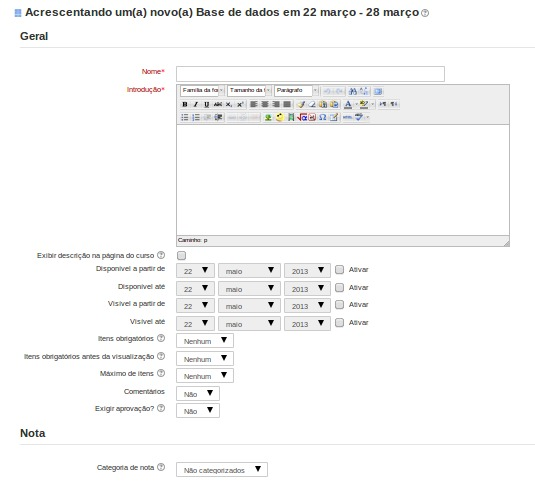
\includegraphics[width=0.7\textwidth]{imagem/cap5/fig1.jpg}}
  \caption{Criando e configurando uma Base de dados}
  \label{fig:cap5_1}
 \end{center}
\end{figure}

Na tabela abaixo, detalharemos melhor os seguintes campos:
\begin{longtable}{p{6cm}|p{9cm}}
   \hline
 \rowcolor[rgb]{0.8,0.8,0.8} \textbf{Campos} &  \textbf{Descrição}\\\hline
 {Nome} & Define o nome ou título da atividade base de dados que será visualizada pelos alunos na página principal do curso.\\\hline
 {Introdução} & Breve descrição da atividade que está sendo criada.\\\hline
 {Disponível a partir de / Disponível até} & Datas entre as quais a base de dados estará disponível para contribuições e consulta.\\\hline
 {Visível a partir de / Visível até} & Datas entre as quais a base estará visível para os alunos.\\\hline
 {Itens obrigatórios} & Número de itens obrigatórios que um participante poderá enviar. Os usuários verão um lembrete e consequentemente a atividade não será finalizada, até que os usuários submetam o número estipulado de itens.\\\hline
 {Itens obrigatórios antes da visualização} & Neste campo você define o número de itens que um usuário deverá enviar antes que lhe seja permitido visualizar qualquer dado disponível na atividade.\\\hline
 {Máximo de itens} & Número máximo de itens que um usuário pode criar nesta atividade.\\\hline
 {Comentários} & Selecionando a opção \textbf{Sim}, possibilita os participantes comentarem cada item. Caso a opção seja \textbf{Não}, desativa a função de comentário.\\\hline
 {Exigir aprovação?} & As entradas devem passar por aprovação do professor antes de serem liberadas aos alunos. Essa função torna-se útil quando há necessidade de mediar à publicação de conteúdos que podem ser potencialmente ofensivos e/ou inadequados.\\\hline
 {Categoria de nota} & se a atividade for avaliativa, deverá ser vinculada a uma categoria de notas.\\\hline
 {Funções com permissão para avaliar:} somente usuários com determinadas funções têm permissão para a avaliação de itens.
 {Tipo agregado} & Neste campo podemos definir como as avaliações são combinadas para formar a nota final. Entre os seguintes métodos de agregação, estão:\\
 & \textbf{Nenhuma avaliação:} a atividade não aparece na planilha de notas;\\
 & \textbf{Média das avaliações:} a média de todas as avaliações dadas para as postagens no fórum;\\
 & \textbf{Contagem das avaliações:} o número de itens avaliados será a nota final;\\
 & \textbf{Avaliação máxima:} a avaliação mais alta é a nota final;\\
 & \textbf{Avaliação mínima:} a menor avaliação é escolhida como a nota final;\\
 & \textbf{Soma das avaliações:} todas as avaliações para cada usuário são somadas.\\\hline

 {Escala} & Define o tipo de escala que será aplicada para a atribuição da nota, essa função será ativada caso tenha acessado uma das opções do campo \textbf{Tipo de Agregação}, com exceção do método \textbf{Nenhuma avaliação}.\\\hline
 {Permitir avaliações para os itens com datas neste intervalo} & Estabelece um período no qual será permitido realizar avaliações.\\\hline
 {Modalidade grupo} & As atividades podem ser separadas em grupos. Estes seriam os grupos separados e grupos visíveis. Se não houver ou não desejar grupos, a opção Nenhum grupo deverá ser mantida. A seguir definiremos as três opções:\\
 & \textbf{Nenhum grupo:}  Não há subgrupos, todos fazem parte de uma grande comunidade;\\
 & \textbf{Grupos separados:}  Cada membro do grupo pode ver apenas seu próprio grupo, os demais são invisíveis;\\
 & \textbf{Grupos visíveis:}   Cada membro do grupo trabalha no seu próprio grupo, mas pode também ver outros grupos.\\\hline
 {Agrupamento (configuração avançada)} & O agrupamento é uma coleção de grupos dentro de um curso. Se um agrupamento é selecionado, os alunos associados aos grupos desse agrupamento poderão trabalhar juntos.\\\hline
 {Visível} & Determina se essa atividade estará visível ou oculta logo após sua criação. Se optar que a atividade seja visível para os alunos escolha a opção \textbf{Mostrar}, ou se optar que a mesma não fique visível, escolha a opção \textbf{Ocultar}.\\\hline
 {Número identificação do módulo} & Identifica a atividade para fins de cálculo de avaliação na planilha de notas, geralmente é utilizado as iniciais das atividades. Se a atividade não estiver inclusa em nenhum cálculo de avaliação então o campo do \textbf{Número de identificação} do módulo pode ser deixado em branco.\\\hline
\end{longtable}


\begin{figure}[htbp]
 \begin{center}
 \fbox{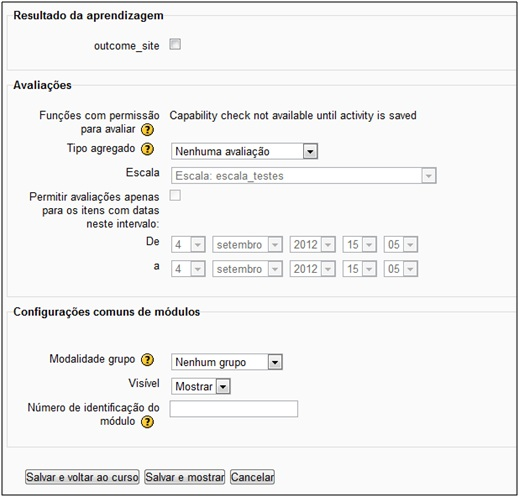
\includegraphics[width=0.5\textwidth]{imagem/cap5/fig2.jpg}}
  \caption{Criando e configurando uma Base de dados}
  \label{fig:cap5_2}
 \end{center}
\end{figure}

Ao fim desses procedimentos, podemos clicar no botão \textbf{Salvar e voltar ao curso}, se deseja salvar a configuração e retornar para página inicial do curso; \textbf{Salvar e mostrar}, se você deseja salvar as configurações e imediatamente visualizar a atividade; ou \textbf{Cancelar}, caso você queira desistir da configuração desta atividade. Ao prosseguir com a configuração da atividade, podemos observar na atividade, a aba superior, no bloco de configurações à esquerda e três campos para a configuração, conforme mostra na Figura \ref{fig:cap5_2}.

\begin{figure}[htbp]
 \begin{center}
 \fbox{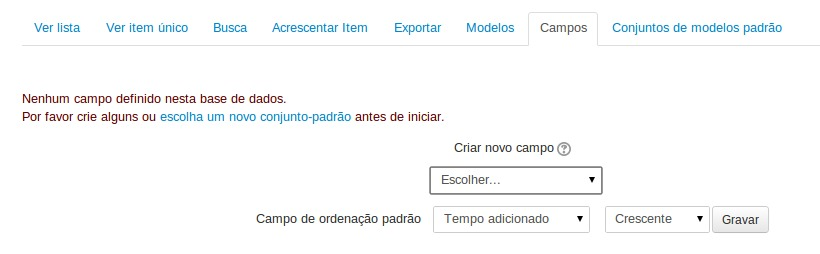
\includegraphics[width=0.7\textwidth]{imagem/cap5/fig3.jpg}}
  \caption{Definindo campos}
  \label{fig:cap5_3}
 \end{center}
\end{figure}

Caso seja necessário reeditar algum detalhe na configuração geral da atividade, devemos clicar no link \textbf{Editar configurações}, indicado à esquerda da figura, no bloco \textbf{Configurações}, item \textbf{Administração de banco de dados de atividade}. Segue ainda, outras opções disponíveis no bloco (Veja a Figura \ref{fig:cap5_2}):

\begin{itemize}
 \item \textbf{Logs:} com o log é possível verificar o relatório das atividades. Essa função permite visualizar os alunos que realizaram a atividade, os que somente a visualizaram, bem como quais alunos não acessaram a atividade.
 \item \textbf{Backup:} realiza o backup (cópia) específico da atividade.
 \item \textbf{Restaurar:} possibilita a restauração do backup realizado nesta mesma atividade.
\end{itemize}

Dando prosseguimento a montagem da base de dados, conforme a Figura \ref{fig:cap5_3} na tela inicial de configuração nos deparamos com uma mensagem indicando que a atividade não possui nenhum campo definido: \textit{Nenhum campo definido nesta base de dados. Por favor, crie alguns ou escolha um novo conjunto-padrão antes de iniciar}.

No item \textbf{Criar novo campo}, selecionamos a opção de acordo com a proposta de sua atividade, a fim de que o usuário possa inserir os dados solicitados na atividade posteriormente.

É importante lembrar que ao criar um novo campo devemos sempre indicar informações necessárias aos usuários, através do campo descrição. Esta informação será incluída na criação e definição dos campos. Na tabela abaixo, serão apresentados alguns campos que podem ser utilizados nesta atividade. Os campos podem ser incluídos e excluídos conforme a necessidade.


\begin{figure}[tbp]
 \begin{center}
 \fbox{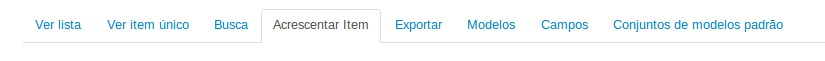
\includegraphics[width=0.9\textwidth]{imagem/cap5/fig4.jpg}}
  \caption{Abas de configuração e visualização}
  \label{fig:cap5_4}
 \end{center}
\end{figure}

\begin{figure}[htbp]
 \begin{center}
 \fbox{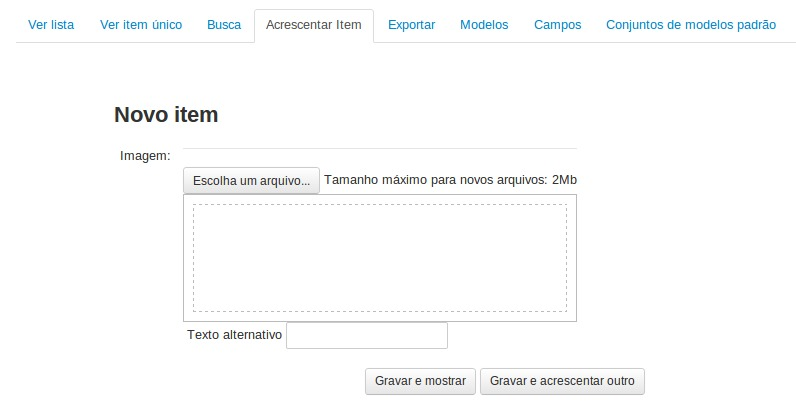
\includegraphics[width=0.7\textwidth]{imagem/cap5/fig5.jpg}}
  \caption{Acrescentar novo item}
  \label{fig:cap5_5}
 \end{center}
\end{figure}


\begin{longtable}{p{6cm}|p{9cm}}
   \hline
 \rowcolor[rgb]{0.8,0.8,0.8} \textbf{Campos} &  \textbf{Descrição}\\\hline
 {Área de texto} & Área para digitação e formatação de texto, no qual o tamanho da caixa de texto (altura e largura) a ser apresentada na base de dados pode ser pré-definido.\\\hline
 {Arquivo} & Botão para envio de arquivo, que possibilita que sejam anexados arquivos de diferentes formatos na base de dados.\\\hline
 {Botões de opção} & Botões de escolha. Permite escolher 1 opção dentre várias alternativas.\\\hline
 {Caixa de seleção} & Função semelhante ao item \textbf{Botões de opção}, porém, permite indicar mais de uma opção.\\\hline
 {Data} & Possibilita inserir uma data no formato Dia/Mês/Ano. Por exemplo, especificar a data de postagem de algum dado.\\\hline
 {Imagem} & Seleção de uma imagem ou envio de uma imagem. Permite escolher o tamanho em lista e item único.\\\hline
 {Latitude/longitude} & Campos para inserção de coordenadas geográficas.\\\hline
 {Menu} & Menu suspenso para escolha de uma opção.\\\hline
 {Menu (múltipla escolha)} & Menu para escolha de múltiplas opções. Deve-se selecionar segurando a tecla \textbf{Ctrl} para escolher mais de 1 item.\\\hline
 {Número} & Campo de texto onde será permitido apenas inserir números.\\\hline
 {Texto} & Campo de texto para caracteres alfanuméricos.\\\hline
 {URL} & Campo de texto para inserção de URLs. Possui opção para fazer o link automático e definir um nome obrigatório para o link.\\\hline
\end{longtable}


% \begin{figure}[htbp]
%  \begin{center}
%  \fbox{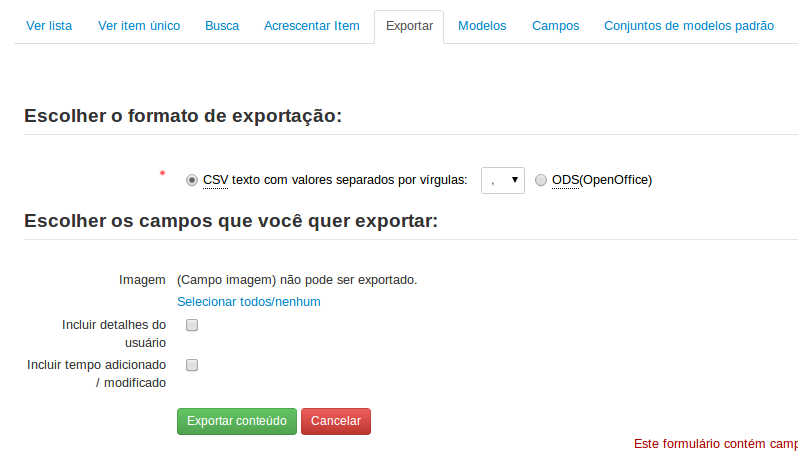
\includegraphics[width=0.6\textwidth]{imagem/cap5/fig6.png}}
%   \caption{Acrescentar novo item}
%   \label{fig:cap5_6}
%  \end{center}
% \end{figure}


Recomendamos que o leitor navegue pelas abas de configuração mostradas na Figura \ref{fig:cap5_4} e detalhadas abaixo:
\begin{longtable}{p{4.5cm}|p{10.5cm}}
   \hline
 \rowcolor[rgb]{0.8,0.8,0.8} \textbf{Campos} &  \textbf{Descrição}\\\hline
  {Ver lista} &  Nesta aba é possível visualizar listagem de itens que foram criados pelos participantes. Ainda, é possível analisá-los detalhadamente, assim como editá-la ou excluí-la, sendo estas duas últimas opções possíveis somente para o usuário que incluiu o item à base de dados ou ao professor.\\\hline
 {Ver item único} & Permite visualizar um arquivo por vez, analisando-os detalhadamente, incluindo os comentários realizados sobre uma das postagens, assim como editá-la ou excluí-la, sendo estas duas últimas opções possíveis somente para o usuário que incluiu o item à base de dados ou ao professor.\\\hline
 {Busca} &  Possibilita realizar uma busca dentre os itens disponíveis na atividade, indicando o(s) termo(s) desejado(s) de acordo com os campos pré-definidos da atividade.\\\hline
 {Acrescentar item} &  Podemos inserir ou acrescentar à atividade os dados definidos inicialmente ao criar os campos, como mostra o exemplo da Figura \ref{fig:cap5_5}, no qual se utilizou os seguintes campos para compor a atividade: \textbf{Data, Arquivo, Imagem, Área de texto e Menu (múltipla escolha)}.\\\hline
 {Exportar} &  Nesta aba é possível exportar componentes de uma base de dados nos formatos, CSV (texto com valores separados por vírgulas) e ODS (OpenOffice), além de possibilitar escolher os itens ou componentes da atividade que serão exportados com exceção do campo \textbf{Arquivo e Imagem Moodle}, com base na Figura \ref{fig:cap5_5}. Para finalizar a operação clique no botão \textbf{Exportar conteúdo}.\\\hline
 
 {Modelos} & Permite controlar a disposição visual das informações quando elas são pesquisadas (aba \textbf{Busca}), visualizadas (abas \textbf{Ver Lista} e \textbf{Ver Item Único}) e na introdução de novas informações (aba \textbf{Acrescentar Item}). A aba modelo está mais direcionada a formatação da atividade, é recomendável manter a formatação inicial. Porém, em todo caso, é possível formatar e a modificar os campos já inseridos, como por exemplo, alterando as configurações de fonte, cor e tamanho. Mas é preciso ter cuidado para não comprometer a programação já feita. Veremos mais informações na sessão \textbf{Configurando Modelos}.\\\hline
 
 {Campos} & Nesta aba é possível escolher os campos de acordo com a necessidade do administrador/professor para apresentação dos tipos de dados a serem visualizados na aba modelos, como texto, arquivos, endereços, links, datas, entre outros. Estes campos são os mesmos inseridos inicialmente na atividade. Caso haja necessidade de inserir mais campo à atividade, basta selecionar a opção \textbf{Criar novo campo}, como na Figura \ref{fig:cap5_7}. Se desejar editar ou excluir um campo já inserido, clique na 
\includegraphics[width=0.02\textwidth]{imagem/cap5/fig7.jpg} para editar e o 
\includegraphics[width=0.02\textwidth]{imagem/cap5/fig8.jpg} para excluir, presentes na coluna \textbf{Ação}.
No entanto, sempre que um campo desta coluna for excluído ou adicionado, deverá restaurar todos os modelos de visualização nos campos de \textbf{Base de dados}. Isso é possível na aba \textbf{Modelos}, conforme será detalhado mais adiante (\textbf{Configurando Modelos}).\\\hline
 
 {Conjuntos de modelos padrão} & Permite importar e exportar modelos da \textbf{Base de dados}. Ao exportar uma base de dados, o modelo aplicado atualmente será salvo sem os dados inserido pelos usuários, apenas com os campos e botões utilizados. Há duas formas de exportar uma \textbf{Base de dados}, a primeira em um formato zip, dessa forma permite que os modelos sejam salvos no computador e enviado mais tarde para outro banco de dados, a outra forma de exportar é como \textbf{Modelo padrão}, que publica os modelos atuais como uma predefinição, sendo que qualquer outro usuário poderá ver ou usar. Para importar um modelo salvo no computador, clique no botão \textbf{Escolha um arquivo} na área \textbf{Importar de arquivo zip}. Selecione o arquivo e clique no botão \textbf{Importar}. Caso deseje carregar um modelo já pronto do Moodle, na área \textbf{Usar um conjunto}, selecione o campo \textbf{Galeria de imagens} e clique no botão \textbf{Escolher}. Muita atenção ao importar uma base de dados, 
antes, verifique se não há nenhum campo já definido na sua base atual, pois caso seja importada uma base que já tenha um modelo editado e definido anteriormente, a base importada será acrescida às etiquetas disponíveis (aba modelo) na base já existente.\\\hline
\end{longtable}


\begin{figure}[htbp]
 \begin{center}
 \fbox{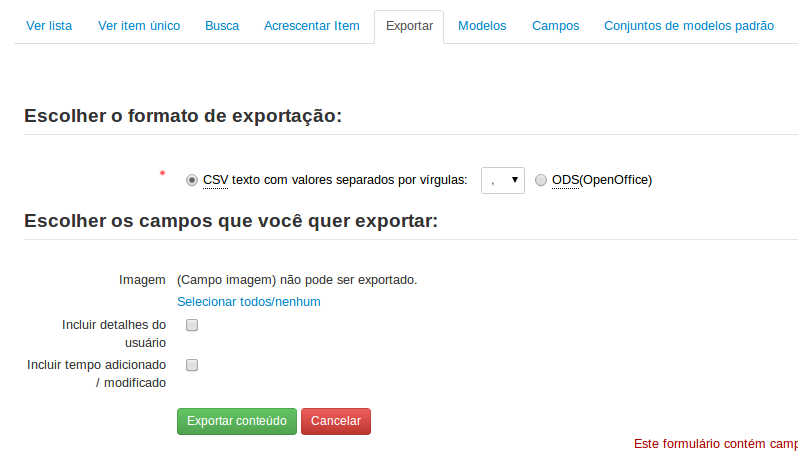
\includegraphics[width=0.7\textwidth]{imagem/cap5/fig6.png}}
  \caption{Exportar conteúdos}
  \label{fig:cap5_7}
 \end{center}
\end{figure}

\subsection{Configurando Modelos}

Após a criação dos campos será a vez de configurarmos os modelos da \textbf{Base de dados}. Estes modelos definem como será a visualização das interfaces correspondentes ao modelo na base de dados pelo usuário. A Figura \ref{fig:cap5_11} mostra a aba \textbf{Modelos} contendo sete links direcionados à configuração das abas e formatos da programação. Após a configuração dos modelos, a base de dados estará pronta para ser utilizada pelos usuários, que poderão acrescentar objetos de aprendizagem à mesma.
\begin{figure}[htbp]
 \begin{center}
 \fbox{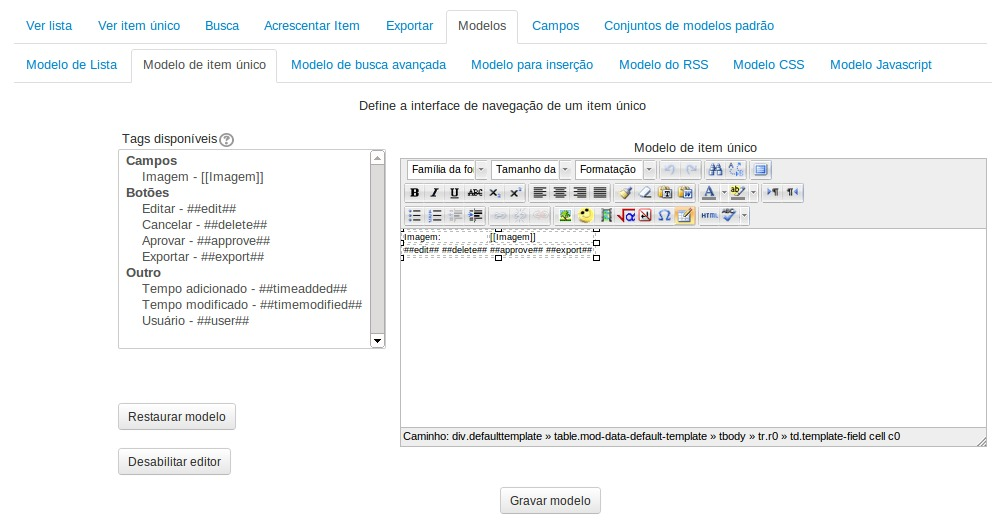
\includegraphics[width=0.7\textwidth]{imagem/cap5/fig11.jpg}}
  \caption{Configuração de Modelos de Exibição}
  \label{fig:cap5_11}
 \end{center}
\end{figure}
Serão abordados aqui, quatro links mais utilizados, ligados especificamente à configuração dos modelos.
\begin{itemize}
 \item \textbf{Modelo de Lista:} define a interface de navegação para listas, a partir da configuração para apresentação dos campos visualizados na aba \textbf{Ver lista}.
 \item \textbf{Modelo item único:} define a interface de navegação de um item único, permitindo possibilidades de configuração para a apresentação dos campos visualizados na aba \textbf{Ver item único}.
 \item \textbf{Modelo de busca avançada:} define a interface de navegação de um item único, permitindo possibilidades de configuração para a apresentação dos campos visualizados na aba \textbf{Busca}.
 \item \textbf{Modelo para inserção:} define a interface para inserção de novos itens, permitindo possibilidades de configuração para a apresentação dos campos visualizados na aba \textbf{Acrescentar Item}.
\end{itemize}

Em cada modelo é possível visualizar o campo de edição e as \textit{tags} (etiquetas) que estão disponíveis em sua configuração. O conjunto de \textit{tags} no modelo correspondem à área em que os campos e botões serão posicionados quando os itens forem editados ou acessados. Os campos serão representados pelo seu nome entre colchetes \textbf{[ ]}; os botões, pelo seu nome entre cerquilhas (\textbf{\#}). Apenas as \textit{tags} presentes na lista podem ser utilizadas no modelo selecionado.
	
Se o objetivo é ocultar a visualização de alguns campos, basta selecionar a linha que representa o nome e o campo, localizados no espaço de edição do modelo, deletando e posteriormente clicando no botão \textbf{Gravar modelo}, no inferior da página. Caso deseje mudar de ideia e queira utilizar todos os campos e botões disponíveis ao modelo, clique no botão \textbf{Restaurar} e após em \textbf{Gravar modelo}. Sempre que algum item no campo de edição for alterado, as modificações só surtirão efeito após clicar no botão \textbf{Gravar modelo}.
	
Ao excluir ou acrescentar um campo da Base de dados, procedimento realizado na aba Campos, devemos sempre restaurar os modelos já existentes. Por exemplo, ao excluir um campo, podemos observar na aba \textbf{Modelos} que os campos ainda permanecem visíveis na área de edição. Para que não fique mais visível na aba desejada, devemos clicar no botão \textbf{Restaurar modelo}, em todos os quatro modelos referidos, que sempre utilizarão como base os campos e botões disponíveis na lista de \textit{tags} e, a seguir, em Gravar modelo.

\textbf{Observação:} Para os usuários com função de \textbf{Estudantes}, estarão disponíveis somente as seguintes abas de configuração: \textbf{Ver Lista, Ver item único, Busca e Acrescentar Item}, porém o usuário que postou o item, somente ele poderá excluir e modificar os dados, sendo este com função de instrutor do curso, poderá excluir qualquer item postado, caso haja necessidade.

\section{Salas de bate-papo (chats)}

O módulo chat do Moodle é uma ferramenta simples de comunicação síncrona que permite uma discussão entre dois ou mais usuários em tempo real. O termo \textit{chat} provém do verbo inglês \textit{To chat} que significa ``tagarelar''. É igualmente o acrônimo de ``\textit{Conversationnal Hypertext Access Technology}''. Em analogia, podemos comparar a uma sala reunião, onde participantes encontram-se em um espaço virtual enviando e recebendo mensagens entre todos os presentes.

O objetivo de um \textit{chat} não é o mesmo que o de um fórum de discussão. O \textit{chat} favorece a comunicação em tempo real entre um grupo de indivíduos e aproxima-se mais de uma comunicação privada, enquanto um fórum de discussão permite a um grande número de indivíduos trocar e consultar a conversa sem necessariamente estar presente no mesmo momento.

\subsection{Criando e configurando um \textit{chat}}

Os primeiros passos para criar uma sala de \textit{chat }são os mesmos utilizados para se criar uma tarefa. Clicar em \textbf{Ativar edição} e, na semana ou tópico desejado, escolher a atividade \textit{chat}. Isso conduz o autor à tela mostrada a baixo.

\begin{figure}[htbp]
 \begin{center}
 \fbox{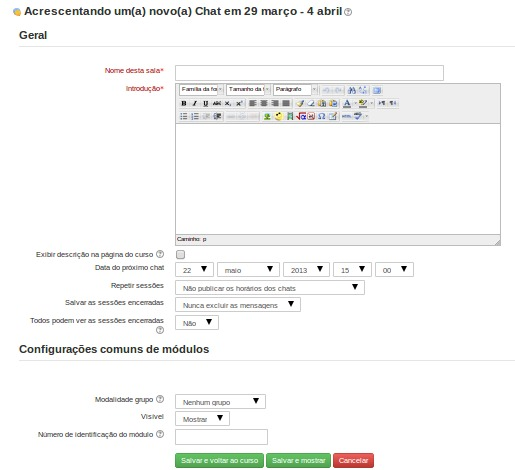
\includegraphics[width=0.7\textwidth]{imagem/cap5/fig12.jpg}}
  \caption{Criando e configurando um \textit{Chat}}
  \label{fig:cap5_12}
 \end{center}
\end{figure}

A configuração geral do \textit{chat} é bem sucinta e descreve-se a seguir:

\begin{itemize}
 \item \textbf{Nome desta sala:} o nome desta sala será visto na página principal pelos participantes. É recomendável a utilização de frases curtas e objetivas que reflita a finalidade do \textit{Chat}.
\item \textbf{Introdução}: instruções gerais da sala \textit{chat} criada. Datas, regras e outras informações relevantes.
\item \textbf{Data do próximo \textit{chat}:} dia e hora da realização da próxima seção de bate-papo.
\item \textbf{Repetir sessões:} São quatro opções.
\subitem \textbf{Não publicar os horários dos chats:} neste caso a sala estará sempre aberta para os participantes presentes na plataforma, portanto, não será mostrado o tempo para iniciar a próxima sessão do \textit{chat}.
\subitem  \textbf{Não repetir:} publicar apenas o horário específico: criar apenas uma sessão, no horário especificado.
\subitem  \textbf{Na mesma hora todos os dias:} cria um aviso no \textbf{Calendário} do curso, com a hora especificada para a sessão diária do chat.
\subitem  \textbf{No mesmo horário cada semana:} cria um aviso no \textbf{Calendário} do curso com o horário semanal do \textit{chat}.
\item \textbf{Salvar as sessões encerradas:} limite de tempo para guardar o histórico das sessões passadas. Sessões mais antigas que o período estipulado serão excluídas. Há também a opção de não excluir os históricos.
\item \textbf{Todos podem ver as sessões encerradas:} se escolhido \textbf{Não}, somente os usuários com permissão para ver o histórico dos chats poderão fazê-lo.
\end{itemize}

As demais informações para configuração do chat são as mesmas já descritas para configurar a atividade \textbf{Tarefa}. Clicando em \textbf{Salvar e voltar ao curso}, as configurações do \textit{chat} serão salvas e voltará para página principal do curso, caso a opção \textbf{Salvar e mostrar} seja escolhida, as informações serão salvas e direcionada à atividade chat.

\subsection{Utilizando \textit{chats}}

Para acessar o \textit{chat} é bastante simples. Ao clicar na atividade de \textit{chat}, disponível na página principal do curso, podemos observar três opções:

\begin{figure}[htbp]
 \begin{center}
 \fbox{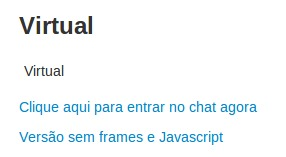
\includegraphics[width=0.35\textwidth]{imagem/cap5/fig13.jpg}}
  \caption{Tela de opções de chat}
  \label{fig:cap5_13}
 \end{center}
\end{figure}

\begin{itemize}
 \item \textbf{Clique aqui para entrar no \textit{chat} agora:} versão padrão do \textit{chat}. Ao clicar nessa opção abrirá uma nova janela mostrando uma estrutura organizada em frames (quadros).
 \item \textbf{Versão sem frames e Javascript:} versão do\textit{chat}para navegadores antigos e que pode ser utilizada com software especial para acessibilidade (por exemplo, leitor de tela para deficientes visuais).
%  \item \textbf{Ver sessões encerradas:} mostra o histórico das sessões de \textit{chat} anteriores.
\end{itemize}

Mesmo que se tenha sido estabelecido um horário para uso de chats, a sala estará sempre aberta para os participantes. O Moodle não restringe o acesso à sala de bate-papo aos períodos que um \textit{chat} tenha sido agendado. A diferença entre escolher estabelecer ou não um horário para o \textit{chat} está no bloco de \textbf{Calendário}, que serve como lembrete de compromisso entre participantes.

A visualização do  \textit{chat } é mostrada na Figura \ref{fig:cap5_14}:

\begin{figure}[htbp]
 \begin{center}
 \fbox{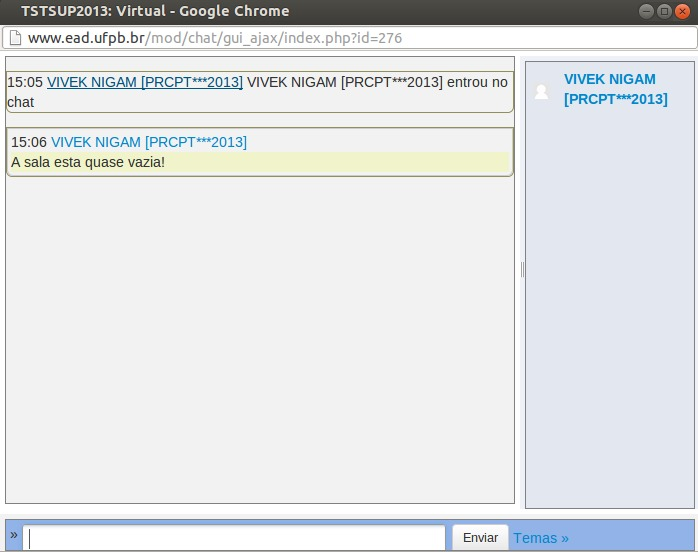
\includegraphics[width=0.7\textwidth]{imagem/cap5/fig14.jpg}}
  \caption{Visualização padrão do chat}
  \label{fig:cap5_14}
 \end{center}
\end{figure}

\begin{enumerate}
 \item Campo de texto para digitar mensagens para o chat.
\item Área com as mensagens da conversa.
\item Lista de participantes do chat.
\item Botão para escolher o tema da interface.
\end{enumerate}

Para enviar uma mensagem, basta digitar no campo de texto “\textbf{1}” e clicar no botão \textbf{Enviar} ou \textbf{pressionando a tecla Enter}, logo em seguida sua mensagem será visível na tela “2”. As mensagens são ordenadas de cima para baixo, da mais antiga para mais recente. Na lista de participantes “3”, abaixo do nome de cada participante, há dois botões especiais: \textbf{Falar} serve para usar o  \textit{chat} de voz quando disponível e \textbf{bip} serve para chamar a atenção de algum outro participante. O Moodle da UFPB Virtual não disponibiliza  \textit{chat} por voz.

A interface da versão sem   \textit{frame} s e Javascript é um pouco diferente (Veja a Figura \ref{fig:cap5_15})

\begin{figure}[htbp]
 \begin{center}
 \fbox{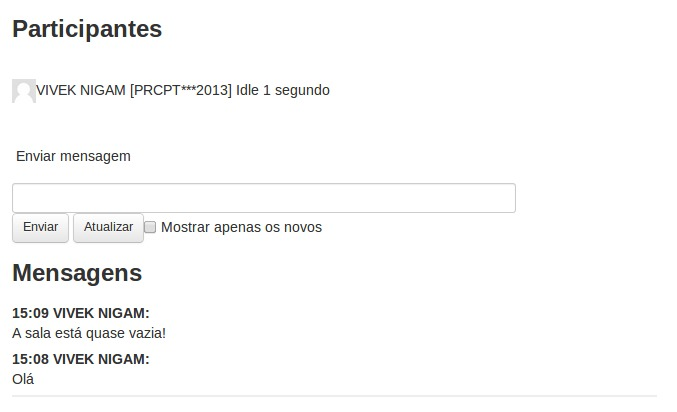
\includegraphics[width=0.5\textwidth]{imagem/cap5/fig15.jpg}}
  \caption{Tela de  \textit{chat} (Versão sem  \textit{frames})}
  \label{fig:cap5_15}
 \end{center}
\end{figure}

\begin{enumerate}
 \item Campo de texto para digitar mensagens para o chat.
\item Área com as mensagens da conversa.
\item	Lista de participantes do chat.
\end{enumerate}

Nesta interface as mensagens são ordenadas de baixo para cima, da mais antiga para a mais nova. É necessário clicar no botão\textbf{ Atualizar} para ver as novas mensagens. Esta interface é muito rudimentar e deve somente ser utilizada em casos especiais, como por exemplo, um software leitor de tela, usado por deficientes visuais. Para obter o melhor desempenho da interface padrão do Chat, é necessário utilizar um navegador Web atualizado.

É possível visualizar o histórico das sessões de chats anteriores clicando em \textbf{Ver sessões encerradas}. As sessões são ordenadas de cima para baixo, da mais recente para a mais antiga.

\subsection{Práticas eficazes para o uso do Chat}

Embora a atividade  \textit{chat} não seja rica em recursos, pode-se usá-la como ferramenta eficaz de aprendizagem.
Existem relatos de um caso de um professor que ficou impedido de falar por um semestre (em virtude de uma cirurgia). Ele manteve seu curso indicando aos alunos os textos a serem lidos e mantendo sessões de chat, no formato perguntas e respostas, no horário em que as aulas seriam dadas presencialmente. Pedia-se aos alunos que comparecessem às sessões de  \textit{chat} com a matéria já estudada.

A chave para uma sessão de  \textit{chat} bem sucedida é a qualidade da moderação. É muito importante anunciar, antes da sessão quem vai ser o moderador, qual o tema a ser discutido e quais as regras de participação. Sem essas providências uma sessão de  \textit{chat} pode tornar-se caótica e nada eficaz.

\subsection{Práticas criativas}

\subsubsection{Atendimento de alunos online}

As horas para atendimento presencial dos alunos podem ser eficazmente substituídas por encontros online. Muitos alunos podem não ter condições (por motivos variados) de comparecer à sala do professor nos horários estabelecidos. A sala de bate-papo pode substituir esses encontros presenciais. O professor pode, por exemplo, estabelecer faixas de horário em que ele estará online na sala de chat. Nesses horários os alunos entram na sala e tiram suas dúvidas.

\subsubsection{Chats por grupo}
Se uma turma de alunos for dividida em grupos, pode-se configurar  \textit{chat} por grupos, visíveis ou separados. Cada grupo pode, assim, discutir seus temas de estudo na sala de  \textit{chat} sem que o número de participantes seja muito grande.

\subsubsection{Dúvidas em véspera de provas}

Pode-se agendar uma sessão de  \textit{chat} para a última semana antes de uma prova final. Os alunos têm, então, a oportunidade de tirar dúvidas de última hora. Isso pode ser muito eficaz para o desempenho de muitos em provas finais.

\subsubsection{Escolhas}

A atividade escolha é uma atividade do Moodle que consiste em uma pergunta única com resposta do tipo múltipla escolha. A configuração básica da escolha consiste em formular uma pergunta e definir as opções que podem ser escolhidas.

A atividade de escolha não pode ser avaliada. É basicamente utilizada para fazer uma pesquisa simples com os participantes a respeito de uma determinada questão. A quantidade de respondentes, de abstenções e a própria resposta são registradas em formato de dados estatísticos no Moodle.

\subsubsection{Criando e configurando a escolha}

Para criar a atividade escolha, devemos clicar em \textbf{Ativar edição}, na página principal do curso, e selecionar a caixa \textbf{Acrescentar atividade} seguida da opção escolha. Aparece a tela mostrada na Figura \ref{fig:cap5_16}.

No campo \textbf{Nome da Escolha}, deverá conter o nome da atividade escolha que será vista pelos alunos. Já no campo \textbf{Introdução} será o próprio enunciado da pergunta a ser respondida.

\begin{figure}[htbp]
 \begin{center}
 \fbox{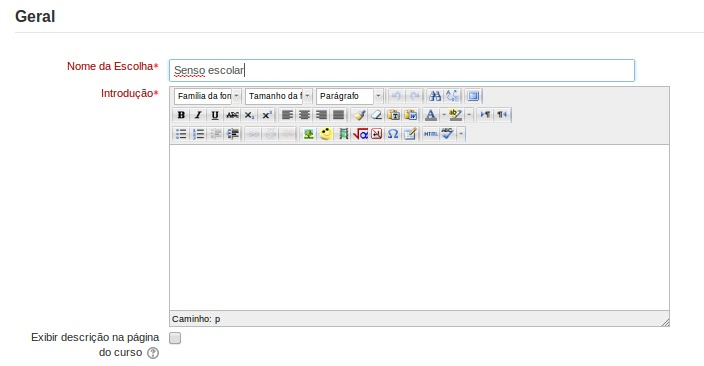
\includegraphics[width=0.6\textwidth]{imagem/cap5/fig16.jpg}}
  \caption{Criando e configurando uma Escolha}
  \label{fig:cap5_16}
 \end{center}
\end{figure}

\begin{figure}[htbp]
 \begin{center}
 \fbox{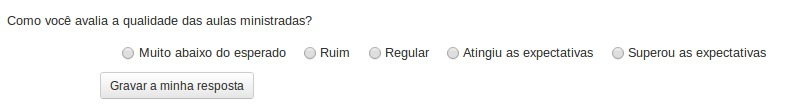
\includegraphics[width=0.6\textwidth]{imagem/cap5/fig17.jpg}}
  \caption{Criando e configurando uma Escolha}
  \label{fig:cap5_17a}
 \end{center}
\end{figure}
Em seguida temos as configurações particulares da Escolha:
\begin{itemize}
 \item Limitar o número de respostas permitidas: limita o número de participantes que podem escolher determinada opção da escolha. Para cada opção poderá ser definida o número de vezes que esta alternativa poderá ser escolhida. Ao atingir o limite, a opção é bloqueada.
 \item Opções: no campo Opção conterá as alternativas que os participantes deverão escolher. Por padrão é apresentado 5 opções, mas também é possível acrescentar o número de alternativas, basta clicar no botão Acrescentar 3 campos ao form. Caso a opção do item anterior esteja ativada, habilitará a função de limitar a quantidade de alternativas respondidas.
 \item Aceitar respostas apenas neste período: quando ativado, a Escolha aceitará respostas somente dentro do período de tempo determinado.

\end{itemize}
Configurações diversas:
\begin{itemize}
 \item \textbf{Formato de visualização:} permite organizar as opções de escolha horizontalmente e verticalmente. Observe as Figuras 4.3 e 4.4.
 \item Publicar resultados: ao publicar os resultados pode-se escolher entre:
    \subitem \textbf{Não mostrar os resultados aos alunos:} essa opção não exibe resultados aos participantes.
    \subitem \textbf{Mostrar os resultados ao estudante só depois que ele tiver dado a sua resposta:} o participante terá de responder a Escolha antes de ver os resultados.
    \subitem \textbf{Mostrar os resultados ao estudante após o fechamento do período de escolha:} após o término do período da Escolha os resultados estarão disponíveis aos participantes.
    \subitem \textbf{Mostrar sempre os resultados aos estudantes:} os resultados estarão sempre visíveis aos participantes.

\end{itemize}

\textbf{Observação:} Com exceção da opção Não mostrar os resultados aos alunos, as demais opções habilita a função de privacidade dos resultados.

\begin{itemize}
 \item 	Privacidade dos resultados:
 \subitem Publicar resultados de forma anônima, sem mostrar o nome do aluno: apenas o número de respostas para cada opção será mostrado.
 \subitem Publicar resultados completos, mostrando os nomes dos alunos e os resultados: mostra o número de repostas e o nome dos participantes.
 \item Permitir a atualização da escolha feita: o participante poderá modificar sua opção de escolha posteriormente.
 \item Mostrar coluna Nenhuma resposta: permite ao participante escolher a opção ‘Nenhuma resposta’.
\end{itemize}

\section{Usando a Escolha}

As próximas figuras a seguir mostram como as escolhas são visualizadas pelos participantes.


\begin{figure}[htbp]
 \begin{center}
 \fbox{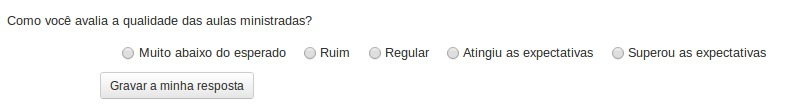
\includegraphics[width=0.6\textwidth]{imagem/cap5/fig17.jpg}}
  \caption{Formato de visualização horizontal}
  \label{fig:cap5_17b}
 \end{center}
\end{figure}

\begin{figure}[htbp]
 \begin{center}
 \fbox{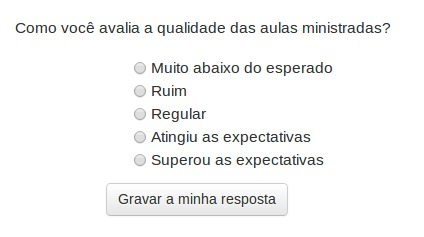
\includegraphics[width=0.6\textwidth]{imagem/cap5/fig18.jpg}}
  \caption{Formato de visualização vertical}
  \label{fig:cap5_18}
 \end{center}
\end{figure}

Os resultados estarão disponíveis aos professores e para alunos dependendo da opção definida em \textbf{publicar os resultados}. Para isto, basta clicar no canto superior direito em \textbf{Ver respostas}. 
\begin{figure}[htbp]
 \begin{center}
 \fbox{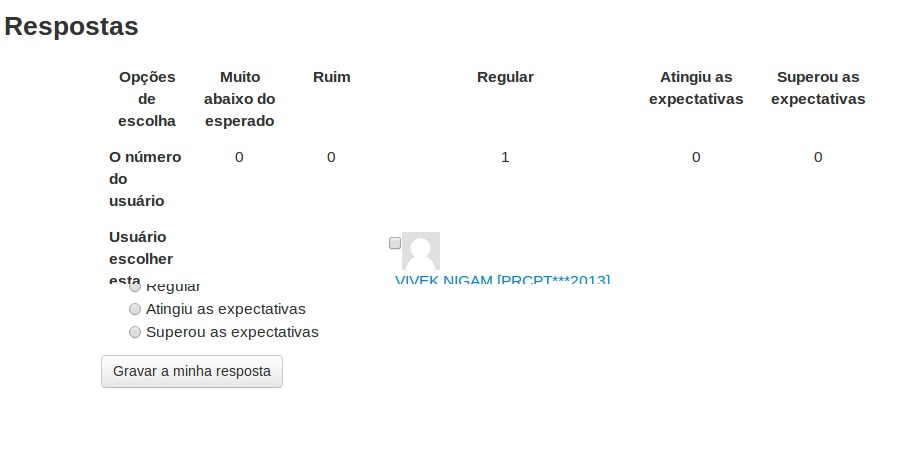
\includegraphics[width=0.6\textwidth]{imagem/cap5/fig19.jpg}}
  \caption{Resultados da Escolha}
  \label{fig:cap5_19}
 \end{center}
\end{figure}

Através desta interface é possível excluir os votos selecionando as repostas desejadas e utilizando a caixa \textbf{Escolha uma ação}. Também há três opções de exportação dos resultados: ODS, Excel e texto simples.

\section{Fórum}

O fórum é uma ferramenta que permite aos participantes de um curso discutir temas de forma organizada e assíncrona. Diferente do Bate-papo, onde os participantes estão presentes e conversando no momento, o fórum funciona como um grande quadro de mensagens, onde cada participante pode deixar sua mensagem no momento que lhes for conveniente. Esta eliminação da “pressão” do tempo permite ao participante uma reflexão mais elaborada sobre o tópico em debate, e permite que alunos ora tímidos em encontros presenciais e alunos de idioma nativo diferente daquele em que o curso é ministrado expressem suas idéias de forma clara e concisa.

Os fóruns foram uma das primeiras aplicações da Internet, na forma dos sistemas BBS (Bulletin Board System). O usuário, usando uma aplicação de BBS, conectava em um servidor usando um modem de linha telefônica e tinha acesso a notícias, mensagens, grupos de discussão etc. O fórum moderno é o sucessor histórico deste antigo sistema, e existem milhões de sites com fóruns sobre os mais diversos assuntos.

É importante que o fórum tenha um assunto bem definido, um fórum sem objetividade fica desorganizado e improdutivo. Cada fórum deve ter tópicos pertinentes ao tema, e cada tópico deve ser formulado de forma a conduzir uma discussão sobre aquilo que se propõe, e nada mais. Um fórum sobre Cálculo Diferencial com um tópico sobre Geometria ficaria confuso. Caberia ao professor colocar esse tópico sobre Geometria em outro fórum, disposto a discutir assuntos interdisciplinares.

Os fóruns no Moodle permitem que os participantes subscrevam-se neles. Ao subscrever-se num fórum, o participante receberá por email as novas mensagens enviadas ao fórum. Para responder as mensagens o participante deve fazer login no ambiente, acessar o fórum, ler as mensagens e responder quando desejado.

\subsection{Tipos de Fórum}
Quando um novo curso é criado, automaticamente é criado o Fórum de Notícias. O fórum de notícias vem com subscrição forçada por padrão, para que todos os participantes do curso recebam as notícias por email. Este fórum pode ser avaliado, mas por padrão não possui avaliação. O Moodle tem tipos de fórum variados que podem servir a diversos propósitos pedagógicos.

\subsubsection{Uma única discussão simples}
Fórum de apenas 1 tópico, simples, usado para manter a discussão focada no tópico escolhido pelo professor.
\subsubsection{Cada usuário inicia apenas um novo tópico}
Neste modo cada participante tem o direito de iniciar apenas 1 tópico, e cada tópico pode ser respondido livremente. Este modo pode ser usado, por exemplo, em uma atividade onde cada aluno deve expor seus pensamentos sobre o tópico da semana.
\subsubsection{Fórum P \& R (perguntas e respostas))}
Este tipo de fórum permite aos participantes postar perguntas a serem respondidas pelos demais. É um fórum onde o participante deve responder à uma pergunta antes de visualizar a resposta dos outros participantes para esta pergunta.
\subsubsection{Fórum geral}
Fórum de propósito geral, onde os participantes podem iniciar tópicos à vontade e responder aos tópicos dos colegas. Este tipo de fórum é muito semelhante aos fóruns da Internet, e são bons quando se deseja uma discussão ampla sobre um assunto. É o tipo de fórum que deve receber mais atenção do professor, uma vez que tópicos duplicados podem dispersar a discussão. Tópicos duplicados tornam o fórum difícil de usar e exige mais administração por parte do professor.
\subsubsection{Fórum padrão exibido em formato de blog}
Funciona da mesma forma que o fórum geral, mas exibe os tópicos como se fossem as postagens em um blog, exibindo a opção de discutir o tópico da mesma forma como se comenta em um blog.
\subsection{Configurando Fóruns}
Ao criar um fórum, há diversas opções a serem configuradas, que permitem adequar o fórum para diversos objetivos. Podemos configurar o tipo de fórum, modo de subscrição, anexos, bloqueio de mensagens, avaliações, configurações de grupo e outras opções. Veja a Figura \ref{fig:cap5_45} que mostra a tela de configuração do fórum.

 \begin{figure}[htbp]
 \begin{center}
 \fbox{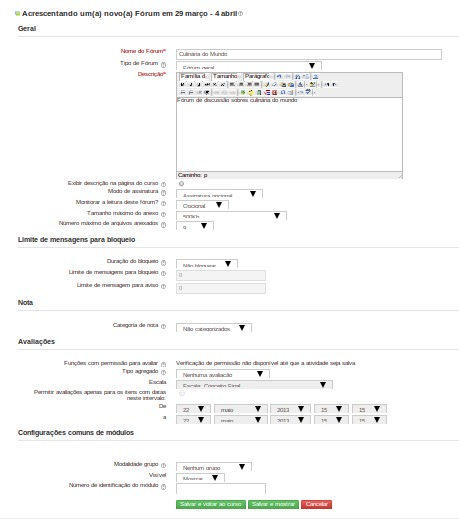
\includegraphics[width=0.6\textwidth]{imagem/cap5/fig45.jpg}}
  \caption{Configurando um Fórum}
  \label{fig:cap5_45}
 \end{center}
\end{figure}

Cada uma das opções de configuração é detalhada a seguir.

\subsubsection{Geral}
Configurações gerais do fórum
\subsubsection{Nome do Fórum}
Este é o nome que aparecerá na página principal do curso para os todos os participantes. Coloque um nome ou frase curta e objetiva que reflita a finalidade do fórum.
\subsubsection{Tipo de fórum}
Para escolher o tipo de fórum a ser usado: Fórum geral, uma única discussão simples, P \& R (perguntas e respostas), cada participante inicia apenas um novo tópico, fórum geral exibido em formato de blog.
\subsubsection{Introdução ao Fórum}
Espaço com editor HTML para redigir a descrição do fórum. Uma boa prática é incluir instruções precisas acerca do assunto do fórum, do critério de avaliação e da escala de avaliação.

Formato HTML: O formato HTML é automaticamente ativado quando no perfil do participante está selecionada a opção “Usar o editor de HTML” na opção “ao editar texto” do perfil do participante. “Usar o editor de HTML” e o formato HTML são ativados por padrão no Moodle 2.1.

\subsubsection{Modo de subscrição}

\textbf{Subscrição opcional:} O participante poderá escolher se quer subscrever ao fórum.

\textbf{Subscrição forçada:} Todos os participantes do curso estão subscritos no fórum.
\textbf{
Auto-subscrição:} Se o participante escolher no seu perfil subscrever automaticamente aos fórum que participa, somente receberá email se começar a participar do fórum.

\textbf{Subscrição desabilitada:} desativa a subscrição de todos os participantes.

\subsubsection{Monitora a leitura deste fórum?}
Esta opção é referente a exibição de mensagens lidas e não lidas no fórum.

\textbf{Opcional:} Permite ao participante escolher, em seu perfil, se deseja monitorar os fóruns.

\textbf{Ativar:} Monitoramento do fórum sempre ativado.

\textbf{Desativar:} Monitoramento do fórum desativado.

\subsubsection{Tamanho máximo do anexo}
Escolhe o tamanho máximo de arquivos anexados a mensagens do fórum. O tamanho máximo é o limite de tamanho de upload do curso. Há também a opção de não permitir anexos.

\subsubsection{Número máximo de arquivos anexados}
Quantidade máxima de arquivos que podem ser anexados a uma mensagem do fórum.

\subsubsection{Limite de mensagens para bloqueio}
É possível bloquear um participante de enviar mensagens a um fórum se este exceder o limite de mensagens em um período determinado. Isto pode evitar o “flood”, ou seja, a “inundação” do fórum com mensagens inapropriadas à discussão.
\subsubsection{Duração do bloqueio}
Período de tempo que conta o número de mensagens e enviadas e a duração do bloqueio
\subsubsection{Limite de mensagens para bloqueio}
Quantidade de mensagens enviadas necessárias para ativar o bloqueio ao fórum.
\subsubsection{Limite de mensagens para aviso}
Quantidade de mensagens enviadas necessárias para avisar ao participante.
\subsubsection{Nota}
Neste campo é possível escolher em qual categoria de nota o fórum se encaixará. As opções disponíveis são as categorias de notas criadas no quadro de notas.

\subsection{Avaliações}
\subsubsection{Funções com permissões para avaliar}
São as funções dentro da disciplina que podem avaliar mensagens no fórum. Essa configuração é feita pelo Suporte.
\subsubsection{Tipo Agregado}
É a forma como o fórum é avaliado.

Nenhuma avaliação: As mensagens do fórum não podem ser avaliadas.

Média das avaliações: Média aritmética de todas as mensagens avaliadas.

Contagem das avaliações: O número de itens avaliados torna-se a nota final do fórum. Observe que esta contagem não podem ser maior que a nota máxima do fórum.

Avaliação máxima: A mensagem com a maior avaliação torna-se a nota final do fórum

Avaliação mínima: A mensagem com menor nota torna-se a nota final do fórum.
Soma das avaliações: A soma de todas as avaliações torna-se a nota final do fórum. Observe que esta soma não pode ser maior que a nota máxima do fórum.
\subsubsection{Escala}
A escala de avaliação pode ser de 1 a 100, nenhuma nota, ou uma das escalas customizadas pelo Suporte no Moodle.
\subsubsection{Restringir avaliações para os itens com datas neste intervalo}
Determina um intervalo de tempo em que somente as mensagens enviadas neste intervalo podem ser avaliadas.
\subsection{Configurações comuns de módulos}
Configurações comuns às diversas atividades.
\subsubsection{Modalidade de grupo}
Escolhe como os grupos funcionarão no fórum: Nenhum grupo, grupos separados ou grupos visíveis.
\subsubsection{Agrupamento}
O agrupamento é uma coleção de grupos dentro de um curso. Se um agrupamento é selecionado, os alunos associados aos grupos desse agrupamento poderão trabalhar juntos.
\subsubsection{Visível}
Se o curso está visível ou não para os participantes.
\subsubsection{Número de identificação do módulo}
Um nome ou número que identifica a atividade no quadro de notas. Este identificador é utilizado no cálculo customizado de notas, como, por exemplo, na Média Final.
\subsection{Utilizando o fórum}
Fóruns consistem em um conjunto de tópicos ou um único tópico, que são apresentados na Figura \ref{fig:cap5_46}.

 \begin{figure}[!htbp]
 \begin{center}
 \fbox{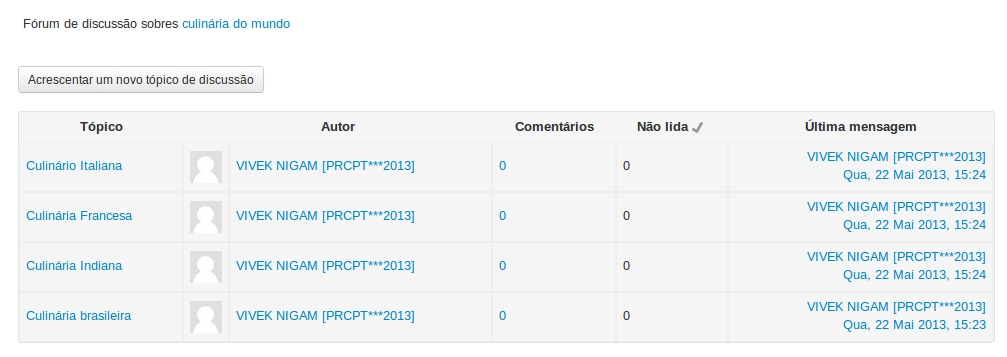
\includegraphics[width=0.7\textwidth]{imagem/cap5/fig46.jpg}}
  \caption{Configurando Fórum}
  \label{fig:cap5_46}
 \end{center}
\end{figure}

\begin{enumerate}
\item Texto de introdução ao Fórum.
\item Botão para criar um novo tópico.
\item Nomes do tópicos.
\item Autores do tópicos.
\item Quantidade de comentários nos tópicos.
\item Data da última mensagem escrita nos tópicos.
\end{enumerate}
Ao clicar no botão para criar um novo tópico é mostrada na Figura \ref{fig:cap5_47}.

 \begin{figure}[!htbp]
 \begin{center}
 \fbox{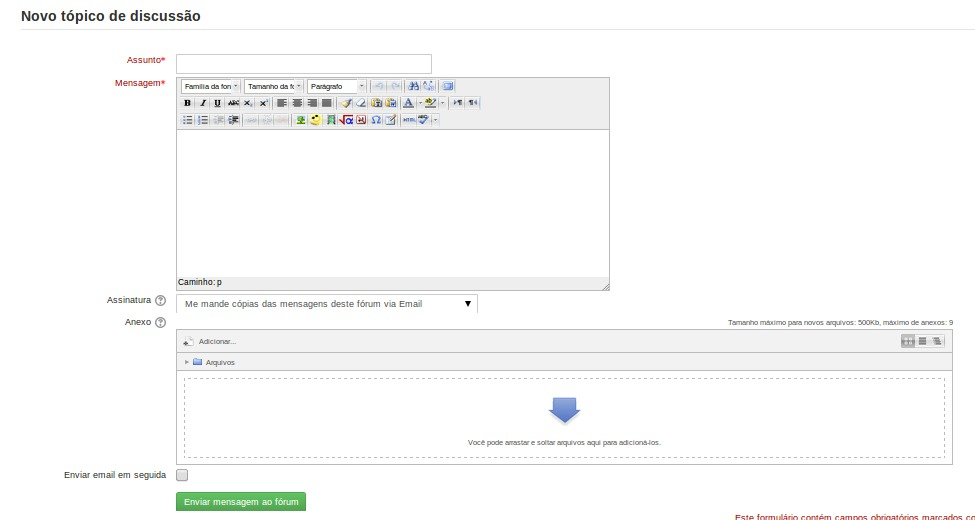
\includegraphics[width=0.7\textwidth]{imagem/cap5/fig47.jpg}}
  \caption{Novo tópico de discursão}
  \label{fig:cap5_47}
 \end{center}
\end{figure}

\begin{enumerate}
\item Assunto: nome do tópico, que será exibido na listagem de tópicos.
\item Mensagem: texto da mensagem do tópico.
\item Subscrição: opção de subscrever ou não ao fórum.
\item Anexo: Botão para anexar um ou mais arquivos.
\item Enviar email em seguida: Envia email notificando os participantes sobre a nova mensagem.
\end{enumerate}

Criado o tópico é possível iniciar a discussão (Figura \ref{fig:cap5_48})

 \begin{figure}[!htbp]
 \begin{center}
 \fbox{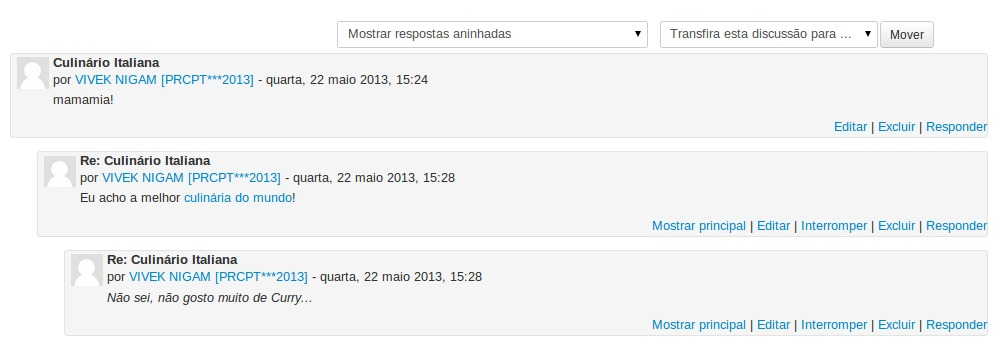
\includegraphics[width=0.6\textwidth]{imagem/cap5/fig48.jpg}}
  \caption{Exemplo de tópico}
  \label{fig:cap5_48}
 \end{center}
\end{figure}
\begin{enumerate}
\item Editar: Modifica a mensagem.
\item Excluir: Remove a mensagem do Fórum definitivamente.
\item Responder: Escreve uma resposta para a mensagem em questão.
\item Avaliação: De acordo com o critério escolhido, mostra o menu de avaliação.
\end{enumerate}
O Moodle mostra as mensagens do Fórum de forma aninhada, para que seja possível visualizar a ordem e a hierarquia das respostas. Assim podemos saber que uma mensagem é resposta de outra resposta, e não da mensagem inicial.

O fórum de uma única discussão simples não exibirá a listagem de tópicos.

\subsection{Buscas no Fórum}
É possível pesquisar nos fóruns através do bloco “Pesquisar nos fóruns” da página inicial do curso, e também usando a ferramenta de busca no canto superior esquerdo do Fórum.
\subsection{Considerações didáticas sobre o Fórum}

Criados os fóruns de um curso é necessário administrá-los. Como já enfatizado, fóruns são uma excelente ferramenta para conseguir a participação de pessoas que usualmente não se manifestam  em encontros presenciais. Se as discussões e a troca de idéias forem um ponto importante de um curso, a participação será de fato conseguida.

O que se deve ter em conta é que muitas pessoas se manifestando em fóruns vai exigir (mesmo que de forma agradável) administração, método e regras. Fóruns podem, com facilidade se degradar. Esta expressão está sendo usada no sentido descrito a seguir.

Fóruns têm um tema central que será discutido em tópicos (fórum = uma coleção de tópicos). Cada tópico, teoricamente, pretende abordar e abrigar o debate  de um aspecto do tema central. No caso de fóruns gerais (todos podem participar e inserir novos tópicos) acontece, com frequência, que um mesmo aspecto seja tratado em dois (ou mais) tópicos diferentes.

\subsection{Administrando expectativas}
A primeira providência para gerenciar um fórum é gerenciar as expectativas dos estudantes. No Plano de Curso (ou Guia do Participante) é importante deixar claro com que frequência o professor pretende participar de fóruns. Quais os objetivos de cada fórum e o que se espera como participação dos alunos.

Em fóruns gerais, com tema determinado, não é interessante que se estabeleça um processo de perguntas e respostas. O mais eficaz é mostrar que os participantes podem criar uma comunidade de aprendizagem  em que todos aprendem e ensinam para todos. Para que isto tenha mais chance de acontecer o enunciado do fórum deve ser claro, conciso e objetivo.

\subsection{Metas de comportamento}
Administrar alunos rudes e sem comportamento social aceitável é outro desafio na administração de fóruns. Muitos participantes podem se expressar em fóruns de maneiras que nunca usariam em encontros presenciais. Comentários rudes ou agressivos podem encerrar uma discussão ou desviar completamente seu rumo.

Para evitar tais situações, é necessário tornar claro, no Plano de Curso e em outros locais do curso (por exemplo uma página web com Regras para participação em fóruns) o que se espera ser o comportamento dos participantes em fóruns. Cole [4] recomenda o uso de avaliações das participações como estratégia para evitar comportamentos inadequados. O professor tem ainda, como último recurso, a opção de excluir (eliminar) uma participação em um tópico de fórum.

\subsection{Arquivando fóruns}

Quando  os tópicos de um fórum se desenvolvem em discussões muito longas, ou mesmo quando o mesmo sub-tema se espalha por dois ou mais tópicos, pode ser boa providência arquivar tópicos repetitivos. Isso pode ser feito criando-se um fórum novo (configurado de forma que os alunos não posam acrescentar novos tópicos de discussão) e transferindo para esse novo fórum tópicos repetitivos de um outro fórum temático geral.

Para tanto, se procede como descrito a seguir.

Criar um fórum, por exemplo, intitulado Fórum arquivo. Esse fórum pode ser criado no topo da coluna central ou no último tópico ou semana.

Ir ao fórum com problemas de repetição ou discussão dispersa ou muito longa e, clicando em um tópico desse tipo, no alto à direita usar o recurso Transferir essa discussão para... e então escolher o Fórum arquivo  como local de transferência.

No fórum temático pode ser boa providência recriar o tópico transferido, com o mesmo nome, e colocar no tópico um resumo da discussão até então ali inexistente, para reiniciar a discussão  com mais objetividade.

Usando um fórum arquivo pode-se manter as discussões disponíveis sem permitir que a perda de foco ou excesso de mensagens afastem outros participantes de contribuir.

Administrar as discussões em fóruns pode ser mais fácil com alguma ajuda. Alguns estudos (veja-se [4]) constatam o benefício de designar grupos de alunos para moderar tópicos de discussão em um ou mais fóruns. Se um grupo de estudantes recebe tal função tornar-se responsável pela moderação da discussão, os estudos citados indicam que o conjunto de debates em fórum assume um caráter muito mais produtivo e eficaz.

\subsection{Práticas eficazes em fóruns}
Fóruns são uma ferramenta muito importante no ambiente Moodle. Eles são a forma básica de comunicação entre alunos e entre alunos e o professor. O Construcionismo social, base teórica do ambiente Moodle, tem como pilares (dentre outros) a discussão e negociação de significados.

Segundo Cole [4], “Boa moderação e uma condução inteligente de tópicos para discussão são mais importantes para o sucesso de um curso que conteúdos estáticos para leitura. O MIT  faz as mesmas declaração em sua iniciativa OpenCourseWare (http://ocw.mit.edu). Cerca de 700 cursos / disciplinas têm seu Plano de Curso, conjuntos de listas de exercícios e notas de aulas estão disponíveis gratuitamente. Esta iniciativa, de acordo com o MIT, não é objeto de preocupação porque o valor real desses cursos / disciplinas está na interação entre alunos e instrutores. Os fóruns em Moodle desempenham esse papel de interação e, quando bem conduzidos, com grande eficácia.”

Conseguir que os estudantes participem de fóruns pode ser um grande desafio. Se um fórum é simplesmente criado e se espera que eles participem pode haver grande desapontamento. Criar um fórum com instruções vagas e superficiais e esperar que a participação aconteça pode não ser boa prática.

\subsection{Iniciando a discussão}
Para muitos alunos e professores iniciar a discussão é a parte mais difícil. Assim que alguém começar é bastante provável que as coisas passem a caminhar bem. Um procedimento que pode ser bastante útil é criar um fórum com caráter de socialização, com tema central dedicado a assuntos não relacionados com o curso / disciplina, e nele colocar algum tipo de icebreaker . Isso estimula a participação e, para iniciantes em Moodle, permite praticar o uso de fóruns (como iniciar novos tópicos, como responder em um tópico já iniciado, etc.).
\subsection{Avaliando em fóruns}
Estabelecer com clareza os objetivos de um fórum é apensa o primeiro passo. Os objetivos do professor em um curso podem diferir significativamente daqueles dos alunos. O professor pode desejar que os alunos se envolvam de maneira intensa com o material de estudo em virtude de seu valor intrníseco. Muitos estudantes, no entanto, estão sobrecarregados, preocupados com notas, e fazendo o mínimo exigido em cada uma das disciplinas que cursam.

Para ajudar a alinhar os objetivos do professor com aqueles dos alunos pode ser útil estabelecer uma estratégia de avaliação considerando a participação dos alunos. Moodle tem algumas ferramentas interessantes para ajudar a gerenciar fóruns com avaliação. Para obter sucesso é necessário deixar bastante claros os critérios de avaliação das participações em fóruns. Deve-se avaliar qualidade e não quantidade.  Um aluno que aparecer em um fórum para dizer “Eu concordo” uma vez por dia não está acrescentando nada ao debate. Outro que coloca uma intervenção significativa uma vez por semana está sendo muito mais colaborativo. É necessário, no entanto, estabelecer um equilíbrio entre avaliar pela qualidade e permitir que a discussão flua sem que o único objetivo seja a nota. Isso é uma arte que se domina com o tempo.

Muitos alunos precisam de tempo e apoio para saber participar de fóruns acadêmicos com eficácia e adequação. Uma breve avaliação das discussões em MySpace, por exemplo, revela uma infinidade de participações que seriam inaceitáveis em um ambiente acadêmico. É necessário ajudar os alunos a perceberem a diferença entre um fórum social e um fórum acadêmico. Espera-se que eles fundamentem suas participações com referências? Espera-se que os pontos de vista de colegas sejam reconhecidos e, depois, criticados? Os argumentos apresentados devem ser estruturados com figuras, pontos de vista de outras pessoas, fatos?

Uma vez estabelecidas e tornadas bastante claras as expectativas do professor pode-se pensar em avaliações com o objetivo de qualificar e intensificar a participação. É uma boa prática dar alguns créditos aos alunos apenas pela participação, mas pontuação máxima deve ficar reservada para participações realmente qualificadas e em consonância com os critérios estabelecidos no enunciado do fórum.
\subsection{Usos criativos de fóruns}
Há uma grande variedade de usos criativos de fóruns. Apresenta-se, a seguir, algumas idéias. Os fóruns em Moodle têm uma flexibilidade muito grande. Isto permite que a criatividade do professor possa ser exercida praticamente sem limites.
\subsubsection{Avaliação pelos pares}
Fóruns são uma ferramenta pouco considerada como ambiente para avaliação pelos pares.

Caso 1: Andy Diament, de West Cornwall, UK, usou fóruns para promover avaliação pelos entre pares. Seus alunos estavam aprendendo como projetar bancos de dados desenvolvendo um projeto real em um período de muitas semanas. A cada semana havia um tópico teórico que deveria ser aplicado ao projeto ainda em desenvolvimento. Trabalhando em grupos de dois, o objetivo era, ao final de cada semana, apresentar ao colegas sua versão do projeto usando os conhecimentos aprendidos. Criou-se então, um fórum, onde as duplas apresentavam (como anexos a uma mensagem) a proposta da semana. As duplas avaliavam mutuamente as propostas e aquela melhor avaliada era adotada por todos para avançar para a etapa seguinte do projeto. Os alunos não somente aprendiam com as propostas dos colegas como avançavam  para a etapa seguinte usando a melhor proposta.
\subsubsection{Fóruns P\&R e a solução de problemas}
Caso 2: John Rodgers, de Ontário, Canadá, usa um fórum do tipo P/R no ensino de matemática. Fóruns P\&R permitem que o professor coloque, como tópicos do fórum, uma ou mais questões que devem ser respondidas pelos alunos antes que vejam as respostas dos colegas. Uma aula começa com o instrutor solicitando aos alunos que resolvam um problema de matemática, identifiquem e corrijam conceitos errados, expliquem o significado de símbolos matemáticos em um determinado contexto ou algum outro tipo de exercício. Os alunos usam de 20 a 40 minutos, em grupos para elaborar uma resposta. Depois que todos apresentam sua solução para o problema apresentado eles podem ver as respostas dos colegas. Em etapa posterior, cada um é convidado a responder um questionário (usando o módulo Questionário) para mostrar que os conceitos envolvidos na solução do problema apresentado, foram consolidados e aperfeiçoados observando as respostas apresentadas pelos colegas.

Este segundo exemplo mostra bem as possibilidades da inclusão de tecnologias no processo ensino / aprendizagem bem como a mudança do papel do professor de distribuidor de informações para orientador da aprendizagem de cada um e de todo um grupo de alunos.
\subsubsection{Entrevistas}
Convidar especialistas para conversar com os alunos de uma disciplina tem sido considerado  um procedimento estimulante e muito útil. No entando, agendar essas conversas sempre foi um problema. Os horários do convidade devem, em geral, ter prioridade. Isso conduz a uma situação em que os alunos teriam que usar horários diferentes do horário normal das aulas para que o encontro possa ser realizado.

Esses problemas podem ser eliminados se um fórum for criado, com duração determinada, para que os alunos e o especialista troquem informações. A maneira mais simples é incluir o convidado como participante do curso.

Alguns convidados podem arguir que não têm disponibilidade de tempo para participar de uma discussão aberta, mesmo que por tempo determinado. Neste caso é possível usar um fórum para que os alunos escolham uma coleção de perguntas que gostariam de fazer e enviá-las ao palestrante convidado. As respostas seriam colocadas no ambiente do curso para os comentários de todos os alunos, já sob supervisão do professor regular da disciplina / curso.
\subsubsection{Debates}
Muitos professorem esperam, com frequência, que um certo de debate ocorra espontaneamente em fóruns. No entanto, é muitas vezes difícil manter a bola rolando. Uma alternativa interessante é organizar os alunos em grupos, enunciar um argumento ou tese e atribuir a cada grupo a tarefa de defender / criticar a proposta ou assertiva feita. As defesas e críticas podem ser avaliadas pela sua qualidade e fundamentação sempre deixando claros os critérios usados para tal avaliação. Tisha Bender [2] discute as vantagens de se usar discussões assíncronas (fóruns) em cursos regulares.
\subsubsection{Perguntas mais frequentes}
Quantas vezes um professor responde a mesma pergunta para três ou mais alunos? É normal que os alunos tenham a mesma pergunta sobre um conceito, sobre como realizar um trabalho ou ainda sobre avaliações. Ou porque não há oportunidade para isso nos encontros presenciais ou mesmo por timidez, a maioria espera o final da aula para fazer, em particular, perguntas sobre esses assuntos. E o professor responde as mesmas perguntas a muitos alunos.

Com o avanços das TICs é comum que alunos conheçam o email do professor e enviem as perguntas por email. O mesmo processo de mesmas respostas para muitos alunos se repete. O email enviado a um aluno não é visto por outros alunos. Um fórum do tipo FAQ resolve esses problemas e, mais que isso, permite que tanto alunos quanto professor elaborem perguntas e respostas com mais concisão, clareza e objetividade, uma vez que em fóruns a comunicação é assíncrona.
\subsubsection{Fórum social}
Embora a maior parte dos fóruns criados em um curso / disciplina tenha como tema algum aspecto importante da matéria estudada, é importante reservar um espaço para que os alunos, de maneira informal, conversem entre si. Um espaço de socialização online. Um fórum social, no formato fórum geral, permite que o grupo de alunos estabeleça vínculos de amizade sem a preocupação de se ater aos conteúdos de estudo e nem mesmo preocupação com avaliações. O fórum social pode também ser usado,  no início de um curso, para atividades quebra-gelo. Todos podem ser convidados, por exemplo, para responder a um tópico do fórum social colocado pelo professor, fazendo uma breve apresentação pessoal. Em curso totalmente online, este procedimento é quase obrigatório e tem consequências muito importantes na formação da roda de aprendizagem.
\section{Glossário}
É parte importante da formação de pessoas em uma área de conhecimento o aprendizado do vocabulário utilizado na áera. Em cada área de estudo os especialistas costumam desenvolver uma linguagem própria para comunicar novas idéias, novos verbetes  e mesmo verbetes existentes assusem um novo significado. Muitos especialistas em uma área percebem ser mesmo difícil a comunicação com novatos e um dos motivos é o vocabulário especializado. Especialistas em computação, por exemplo, desenvolveram uma rica coleção de acrônimos, substantivos e abreviações que permitem comunicação rápida mas tornam impossível o acompanhamento de uma conversa entre eles por leigos no assunto.

O Moodle tem uma ferramenta (atividade) dedicada à construção de dicionários que facilitam a comunicação entre professor e alunos e entre alunos. O glossário permite várias configurações e alternativas que tornam fácil a construção coletiva de uma coleção de termos usualmente empregados na área de estudo. Em uma disciplina, é possível ter um glossário principal e vários glossários secundários. Somente professores podem alterar o glossário principal. Pode-se exportar verbetes de glossários secundários para o glossário principal.
\subsection{Configurando o glossário}
Após definir o nome do glossário e o texto de introdução, temos as configurações gerais do glossário (Figura \ref{fig:cap5_49}).
\begin{figure}[htbp]
 \begin{center}
 \fbox{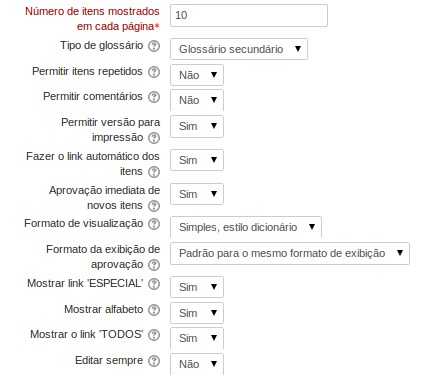
\includegraphics[width=0.4\textwidth]{imagem/cap5/fig49.jpg}}
  \caption{Configuração de Glossário}
  \label{fig:cap5_49}
 \end{center}
\end{figure}
\subsubsection{Número de itens mostrados em cada página}
Quantidade de entradas a serem exibidas por página.
\subsubsection{Tipo de glossário}
Define se o glossário será Principal ou Secundário. Pode-se exportar itens dos glossários secundários para o principal.
\subsubsection{Permitir itens repetidos}
Permite mais de um item com o mesmo nome.
\subsubsection{Permitir comentários}
Habilita comentários para os itens.
\subsubsection{Permitir versão para impressão}
Permite aos estudantes uma visualização do glossário otimizada para impressão.
\subsubsection{Fazer o link automático dos itens}
Habilita a criação automática de links que levam aos itens do glossário sempre que as palavras ou frases definidas como itens estiverem presentes nos textos do curso. Isto inclui as mensagens do fórum, materiais do curso, sumários das semanas, diários, etc.

Se você não quiser que um texto tenha links, você deve adicionar os tags <nolink> e </nolink> ao redor do texto.

Os nomes das categorias também dão origem a links nos textos.
\subsubsection{Aprovação imediata de novos itens}
Esta configuração permite que o professor defina se novos itens acrescentados pelos participantes serão automaticamente disponibilizados para todos, ou se é necessária a aprovação do professor para a publicação de cada item.
\subsubsection{Formato de visualização}
Esta configuração define o modo em que cada item será visualizado no glossário. Os formatos predefinidos são:

\begin{itemize}
\item \textbf{Dicionário simples:}
Um dicionário convencional com os itens separados; os autores não são indicados e os anexos são mostrados como links.

\item \textbf{Contínuo sem autor:}
Mostra os itens um após o outro sem qualquer tipo de separação além dos ícones de edição.

\item \textbf{Completo com Autor:}
Visualiza os itens com o mesmo formato de um fórum, incluindo os dados do autor; os anexos são mostrados como links.

\item \textbf{Completo sem Autor:}
Visualiza os itens com o mesmo formato de um fórum, sem os dados do autor; os anexos são mostrados como links.

\item \textbf{Enciclopédia:}
Mesmas características do formato 'Completo com Autor' mas as imagens anexadas são visualizadas no texto.

\item \textbf{Lista de itens:}
Lista os conceitos como links.

\item \textbf{FAQ:}
Edita items como listas de Perguntas Frequentes (FAQ) e anexa as palavras PERGUNTA e RESPOSTA respectivamente ao conceito e à definição.
\end{itemize}
\subsubsection{Mostrar link ‘ESPECIAL’}
Habilita ou desabilita o menu de navegação por caracteres especiais tais como \@, \#, etc.
\subsubsection{Mostrar alfabeto}
 Habilita ou desabilita o menu de navegação por letras do alfabeto.
\subsubsection{Mostrar o link ‘TODOS’}
Habilita ou desabilita a navegação de todos os itens de uma só vez.
\subsubsection{Editar sempre}
Habilitado, permite aos estudantes editar itens  fora do período permitido.
A configuração de notas é feita como nas demais atividades.
\subsection{Inserindo um novo item no glossário}
Um item do glossário é composto basicamente de dois campos: Conceito e Definição. No Conceito inserimos um termo ou expressão que será explicado na Definição. Para inserir um item primeiramente clica-se no botão ‘Inserir novo item’ (Figura \ref{fig:cap5_50}).
\begin{figure}[htbp]
 \begin{center}
 \fbox{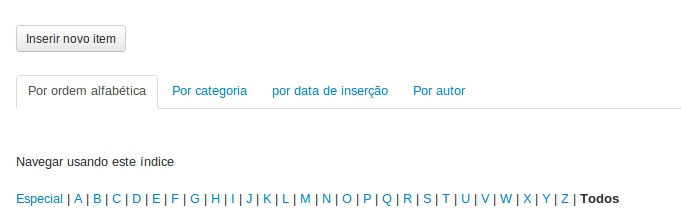
\includegraphics[width=0.5\textwidth]{imagem/cap5/fig50.jpg}}
  \caption{Inserindo glossário}
  \label{fig:cap5_50}
 \end{center}
\end{figure}
Nas Figuras \ref{fig:cap5_51} e \ref{fig:cap5_52}, temos a interface de inserção de item.
\begin{figure}[htbp]
 \begin{center}
 \fbox{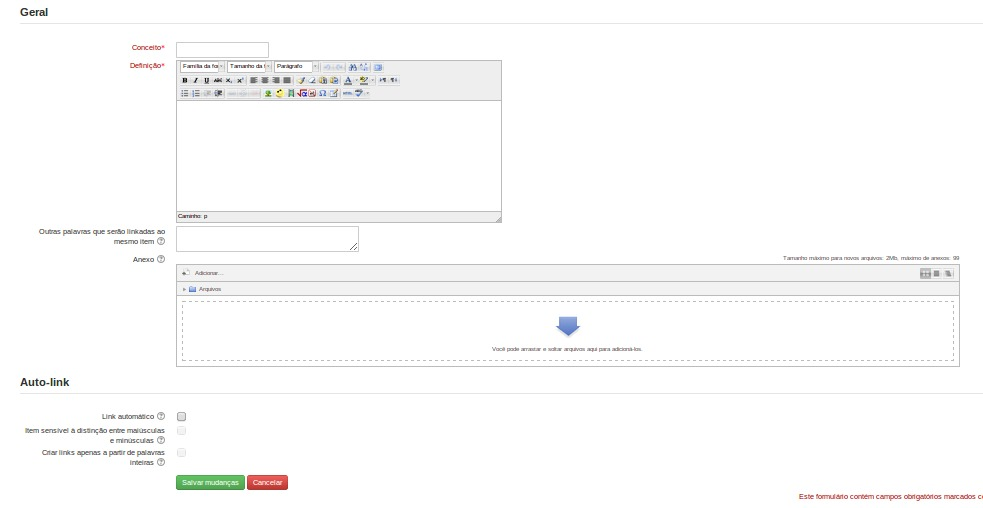
\includegraphics[width=0.7\textwidth]{imagem/cap5/fig51.jpg}}
  \caption{Consifurando glossário}
  \label{fig:cap5_51}
 \end{center}
\end{figure}

\begin{figure}[htbp]
 \begin{center}
 \fbox{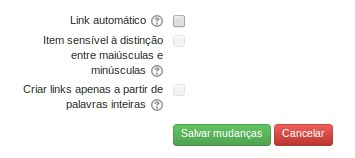
\includegraphics[width=0.5\textwidth]{imagem/cap5/fig52.jpg}}
  \caption{auto-link de glossário}
  \label{fig:cap5_52}
 \end{center}
\end{figure}
Após inserirmos o Conceito e a Definição, temos as demais configurações do item.Outras palavras que serão linkadas ao item. Cada item do glossário pode ser associado a uma lista de palavras-chave (ou aliases).

Deve-se então escrever cada alias em uma nova linha (sem separar com vírgulas). Estas palavras-chave podem ser usadas como referências alternativas ao item associado. Por exemplo, todas estas palavras chave serão linkadas automaticamente ao mesmo item do glossário em caso de criação automática de links (filtro auto-linking).

\subsubsection{Anexo}
Campo para anexar um arquivo, obedecendo ao tamanho limite da disciplina.
\subsubsection{Link automático}
Quando esta função está ativada é possível criar links automáticos aos itens do glossário toda vez que o conceito/título aparecer em textos do mesmo curso. Isto inclui mensagens em fóruns, materiais, sumários, etc.

Para evitar que sejam criados links em um texto específico é necessário adicionar as tags <nolink> e </nolink> antes e depois do texto em questão.

Esta função só é aplicada quando a criação automática de links é ativada no painel de configuração do glossário respectivo.

\subsubsection{Item sensível à distinção entre maiúsculas e minúsculas}
Esta opção define se a criação automática de links a estes itens do glossário deve estabelecer uma correspondência exata entre as palavras, considerando as diferenças entre maiúsculas e minúsculas.

Por exemplo: se esta opção for habilitada, uma palavra como "html" em uma mensagem do fórum NÃO será linkada a um item do glossário chamado "HTML".
\subsubsection{Criar links apenas a partir de palavras inteiras}
Se ativada, esta opção estabelece que os links criados automaticamente devem ser associados apenas a palavras inteiras

Por exemplo: um item chamado "carro" não dará origem a um link incluído na palavra "carroça".

\section{Laboratório de Avaliação}
O Laboratório de avaliação é uma atividade que permite o envio de documentos pelos estudantes, onde os alunos da disciplina têm acesso a todos os documentos enviados e podem avaliar uns aos outros. O papel do professor nesta atividade é de administrar e atribuir notas à avaliação feita pelos estudantes. Esta atividade suporta uma grande variedade de critérios de avaliação. O professor pode disponibilizar documentos como exemplo para que os alunos pratiquem a avaliação. O Laboratório de avaliação está dividido em cinco fases: configurar fase, fase de envio, fase de avaliação, grading evaluation fase e encerrado.
\subsection{Configurando o laboratório de avaliação}
Para adicionar a atividade laboratório de avaliação, deve-se na disciplina desejada, clicar no botão ativar adição. E então na semana ou tópico desejado, selecionar laboratório de avaliação. Podemos acompanhar esse procedimento a seguir na Figura \ref{fig:config_lab}.

\begin{figure}
 \begin{center}
 \fbox{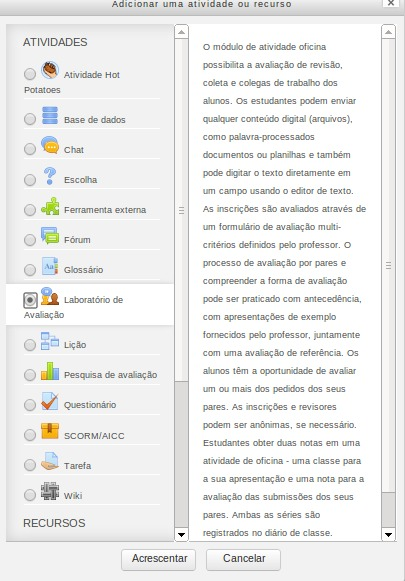
\includegraphics[width=0.35\textwidth]{imagem/cap5/fig64.jpg}}
  \caption{Acrescentando um laboratório de avaliação}
  \label{fig:config_lab}
 \end{center}
\end{figure}

No passo seguinte encontra-se um formulário, que deve ser preenchido obrigatoriamente nos campos nome do workshop (nome da atividade que ficará visível na plataforma) e introdução (informações gerais sobre a atividade Laboratório de Avaliação).

Na aba recursos do workshop (Figura \ref{fig:recursos_work}), pode-se marcar a caixa de seleção em:

\begin{itemize}
 \item “usar exemplos” se desejar submeter um ou mais arquivos como exemplo de como os alunos deverão enviar seus trabalhos.
 \item “use peer assessment” se desejar que os alunos possam avaliar o trabalho dos demais estudantes.
 \item “usar auto-avaliação” se desejar que os alunos possam avaliar seus próprios trabalhos.
\end{itemize}

\begin{figure}
 \begin{center}
 \fbox{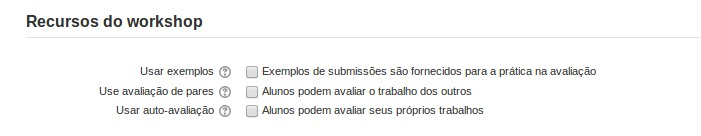
\includegraphics[width=0.6\textwidth]{imagem/cap5/fig65.jpg}}
  \caption{Recursos do workshop}
  \label{fig:recursos_work}
 \end{center}
\end{figure}

Na aba configurações de nota (Figura \ref{fig:config_nota}), pode-se informar em “Nota para envio” a nota máxima que pode ser obtida e a categoria do quadro de notas associada à mesma. Em “Grade de notas” defini-se a nota máxima que pode ser obtida em cada avaliação. No item em “Grading strategy” a estratégia de avaliação a ser utilizada pode ser definida em um dos seguites itens:

\begin{itemize}
 \item Nota acumulativa: comentários e uma nota são dados sobre aspectos específicos;
 \item Comentários - Os comentários são dados sobre aspectos específicos, mas nenhuma nota pode ser atribuída.
 \item Número de erros - Comentários e a seleção de sim/não podem ser avaliados sobre as afirmações especificas;
 \item Rubrica - Um nível de avaliação é dado sobre critérios especificados.
 \end{itemize}

 \begin{figure}
 \begin{center}
 \fbox{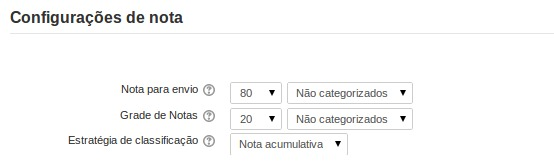
\includegraphics[width=0.5\textwidth]{imagem/cap5/fig66.jpg}}
  \caption{Configurações de nota}
  \label{fig:config_nota}
 \end{center}
\end{figure}

No item configurações de envio (Figura \ref{fig:config_envio}) deve-se preencher o campo “instruções para envio” com informações específicas como quantidade, nome(s), tamanho(s), tipo(s), cores etc. Logo após selecionar o número máximo de anexos enviados, o tamanho máximo de cada arquivo a ser enviado e por fim quando clicar em “Mostrar avançado” pode-se marcar a caixa de seleção “envios atrasados” caso seja necessário permitir o envio de arquivos após o período de tempo estabelecido.

 \begin{figure}
 \begin{center}
 \fbox{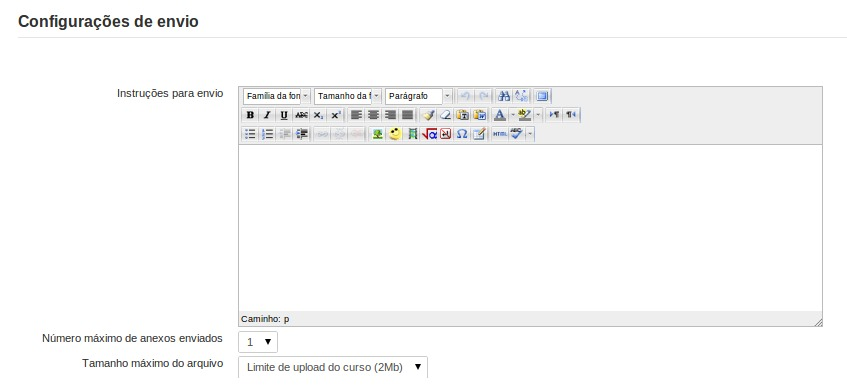
\includegraphics[width=0.5\textwidth]{imagem/cap5/fig67.jpg}}
  \caption{Configurações de envio}
  \label{fig:config_envio}
 \end{center}
\end{figure}

No item configurações de avaliação (Figura \ref{fig:config_ava})temos alguns subitens como “instruções para avaliação” e ao clicar em “Mostrar avançado” podem visualizar “modo de avaliação de exemplos”, caso a opção “usar exemplos” tenha sido marcado anteriormente.

 \begin{figure}
 \begin{center}
 \fbox{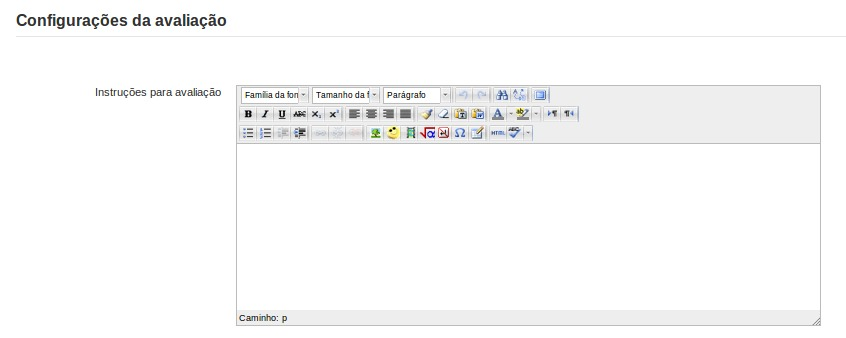
\includegraphics[width=0.5\textwidth]{imagem/cap5/fig68.jpg}}
  \caption{Configurações de avaliação}
  \label{fig:config_ava}
 \end{center}
\end{figure}

No item “controle de acesso” (Figura \ref{fig:controle_acess}) ao clicar em “Mostrar avançado” pode-se visualizar as opções onde será necessário definir a data o horário dos seguintes itens:

\begin{itemize}
 \item Início dos envios: Data e hora do início do envio dos arquivos;
 \item Prazo dos envios: Data e hora final para envio dos arquivos;
 \item Aberto a partir de: Data e hora para início das avaliações;
 \item Prazo da avaliação: Data e hora para o fim das avaliações;
\end{itemize}

\begin{figure}
 \begin{center}
 \fbox{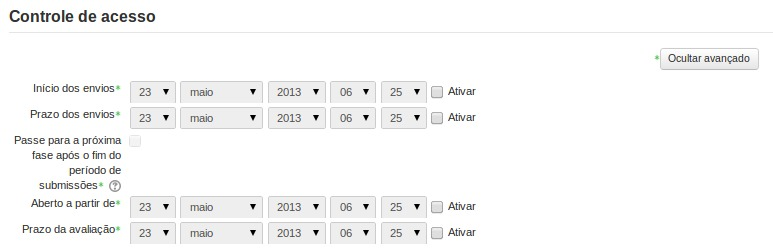
\includegraphics[width=0.6\textwidth]{imagem/cap5/fig69.jpg}}
  \caption{Controle de acesso}
  \label{fig:controle_acess}
 \end{center}
\end{figure}

No item Configurações comuns de módulos (Figura \ref{fig:controle_comum}), no item “Modalidade grupo” deve-se definir uma das seguintes opções:

\begin{itemize}
 \item Nenhum grupo: Não há subgrupos, todos fazem parte de uma grande comunidade.
 \item Grupos separados - Cada membro de grupo pode visualizar apenas seu próprio grupo.
 \item Grupos visíveis - Cada membro do grupo trabalha no seu próprio grupo, mas também pode visualizar outros grupos.
\end{itemize}

\begin{figure}
 \begin{center}
 \fbox{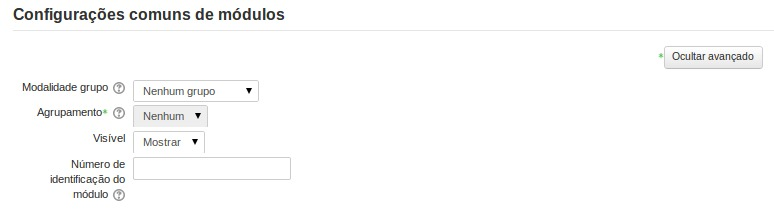
\includegraphics[width=0.6\textwidth]{imagem/cap5/fig70.jpg}}
  \caption{Configurações comuns de módulos}
  \label{fig:controle_comum}
 \end{center}
\end{figure}

Quando clicar em “Mostrar avançado” pode-se então definir o “Agrupamento”, caso exista, além disto, temos o item “visível” para definir se a atividade ficará visível ou oculta para os estudantes e caso seja necessário, preencher o número de identificação do módulo para fins de avaliação.

Para dar continuidade a criação da atividade Laboratório de Avaliação, deve-se salvar o procedimento e logo após esse comando proceder com a edição do formulário de avaliação. Neste formulário serão definidos pelo professor os aspectos a serem avaliados em relação aos arquivos enviados pelos alunos. O formulário de avaliação varia de acordo com o a opção “Grading strategy”, definida no passo anterior dentro do item configurações de nota. Para cada opção disponível (nota acumulativa, comentários, número de erros e rubrica) um tipo diferente de formulário de avaliação é exibido.

Para preencher o formulário de avaliação, deve-se retornar ao curso onde foram realizados os procedimentos anteriores e clicar sobre a atividade Laboratório de Avaliação criada. Será exibida uma imagem semelhante à figura a seguir:

\begin{figure}[htbp]
 \begin{center}
 \fbox{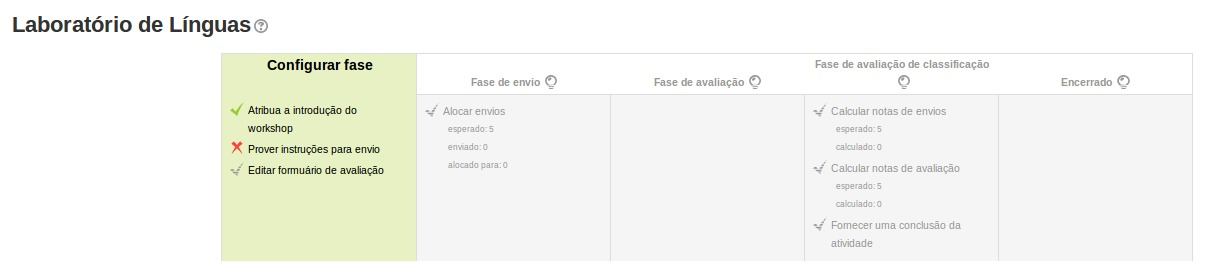
\includegraphics[width=0.5\textwidth]{imagem/cap5/fig71.jpg}}
  \caption{Edição do laboratório de avaliação}
  \label{fig:edit_lab_ava}
 \end{center}
\end{figure}

Na aba “Configuração fase” deve-se clicar em “editar formulário de avaliação”, em seguida será exibido o formulário de acordo com a opção “Grading strategy” selecionada. Se o item selecionado foi nota acumulativa (Figura \ref{fig:item_nota_acumulativa}), será exibido um formulário com os campos semelhantes à Figura \ref{fig:edit_lab_ava}.

\begin{figure}[htbp]
 \begin{center}
 \fbox{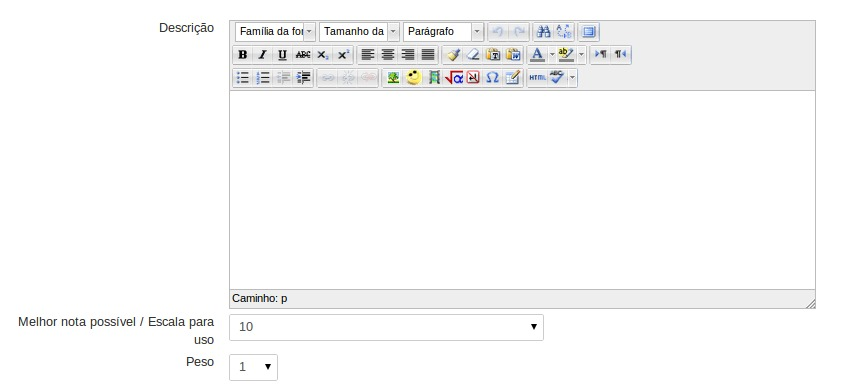
\includegraphics[width=0.5\textwidth]{imagem/cap5/fig72.jpg}}
  \caption{Item nota acumulativa}
  \label{fig:item_nota_acumulativa}
 \end{center}
\end{figure}

Para cada aspecto a ser avaliado, escrever uma breve descrição, informar a maior nota possível para o aspecto e definir um peso para a nota. Por padrão são exibidos três aspectos, porém, caso seja necessário, é possível adicionar mais aspectos de avaliação clicando-se no botão “Em branco para mais 2 aspectos”. Para finalizar o preenchimento do formulário de avaliação, deve-se clicar no botão salvar.

Se o item escolhido foi comentários será exibido um formulário com os campos semelhantes à Figura \ref{fig:item_comentario}. Para cada aspecto a ser avaliado, escrever uma breve descrição. Por padrão são exibidos três aspectos, porém, caso seja necessário, é possível adicionar mais aspectos de avaliação clicando-se no botão “Em branco para mais 2 aspectos”. Para finalizar o preenchimento do formulário de avaliação, deve-se clicar no botão salvar.

\begin{figure}[htbp]
 \begin{center}
 \fbox{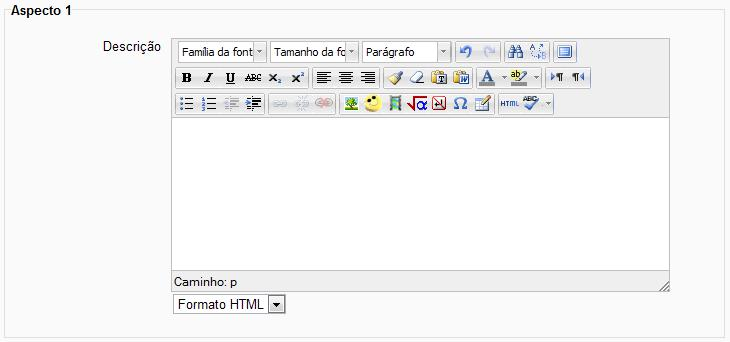
\includegraphics[width=0.5\textwidth]{imagem/cap4_/fig_10.jpg}}
  \caption{Item comentário}
  \label{fig:item_comentario}
 \end{center}
\end{figure}


Se o item escolhido foi número de erros será exibido um formulário com os campos semelhantes à Figura \ref{fig:item_numero_erro}. Neste tipo de formulário, devem-se elaborar afirmações a cerca dos arquivos enviados pelos estudantes. Para cada afirmação, deve-se estabelecer uma palavra para o erro e outra para o acerto (por exemplo, sim ou não), além de um peso.

\begin{figure}[htbp]
 \begin{center}
 \fbox{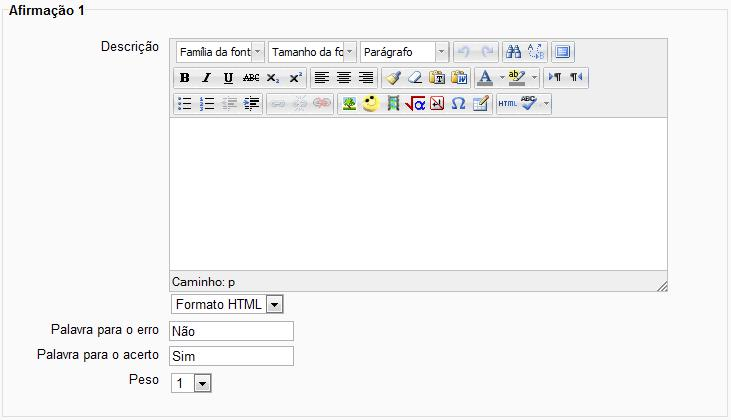
\includegraphics[width=0.5\textwidth]{imagem/cap4_/fig_11.jpg}}
  \caption{Item número de erro}
  \label{fig:item_numero_erro}
 \end{center}
\end{figure}

Por padrão são exibidas três afirmações, porém, caso seja necessário, é possível adicionar mais aspectos de avaliação clicando-se no botão “Em branco para mais 2 aspectos”. Para finalizar o preenchimento do formulário de avaliação, deve-se clicar no botão salvar.

\begin{figure}[htbp]
 \begin{center}
 \fbox{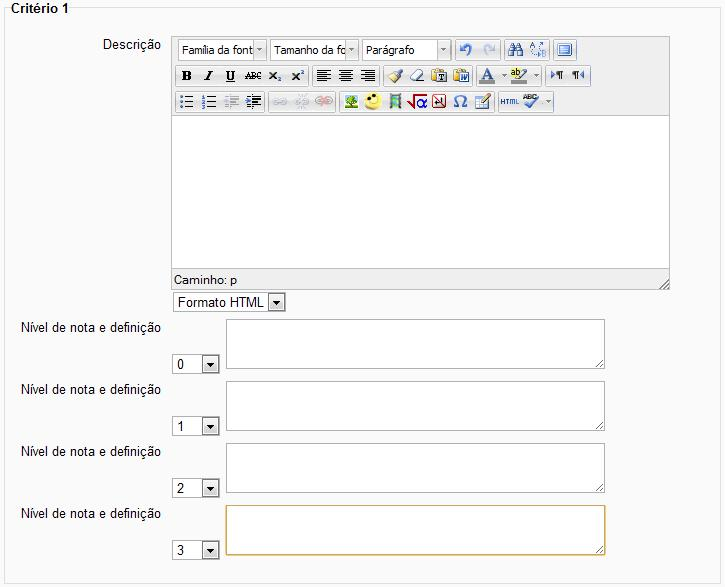
\includegraphics[width=0.5\textwidth]{imagem/cap4_/fig_12.jpg}}
  \caption{Critérios de avaliação}
  \label{fig:criterios_ava}
 \end{center}
\end{figure}

Se o item escolhido foi rubrica será exibido um formulário com os campos semelhantes à imagem anterior. Neste tipo de formulário, devem-se elaborar critérios de avaliação (Figura \ref{fig:criterios_ava}). Para cada critério, devem-se estabelecer comentários que indiquem níveis de elaboração, além de uma nota associada a cada nível. Não é obrigatório o preenchimento dos quatro níveis apresentados no formulário, em outras palavras, podem-se preencher dois ou três, de acordo com a necessidade da atividade.

Por padrão são exibidos três critérios, porém, caso seja necessário, é possível adicionar mais aspectos de avaliação clicando-se no botão “Em branco para mais 2 aspectos”.

O modo de exibição do formulário de avaliação da rubrica pode ser definido de duas maneiras: grade ou lista. Esta seleção do modo de exibição pode ser realizada no final do preenchimento do formulário, conforme Figura \ref{fig:config_rubrica}.

\begin{figure}[htbp]
 \begin{center}
 \fbox{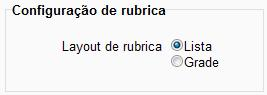
\includegraphics[width=0.5\textwidth]{imagem/cap4_/fig_13.jpg}}
  \caption{Configuração de rubrica}
  \label{fig:config_rubrica}
 \end{center}
\end{figure}

Para finalizar o preenchimento do formulário de avaliação, deve-se clicar no botão salvar e sair.

Após a conclusão da escolha e do preenchimento do formulário adequado, é necessária a criação e o envio de arquivos de exemplo para que os estudantes possam tomar como base para a elaboração de seus trabalhos antes de enviar seus arquivos. É importante ressaltar que o envio de exemplos só é possível se a opção “usar exemplos” for selecionada no início da criação desta atividade. Para adicionar arquivos exemplo a esta atividade, após a conclusão do preenchimento do formulário de avaliação, a opção “Exemplo de tarefa enviada” é habilitada. Para adicionar um arquivo de exemplo, basta clicar no botão “Adicionar exemplo de tarefa enviada”, conforme a Figura \ref{fig:exe_tarefas}.

\begin{figure}[htbp]
 \begin{center}
 \fbox{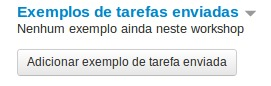
\includegraphics[width=0.3\textwidth]{imagem/cap5/fig74.jpg}}
  \caption{Exemplos de tarefas enviadas}
  \label{fig:exe_tarefas}
 \end{center}
\end{figure}

Em seguida deve-se preencher o formulário de tarefa enviada, informando um título para o exemplo e clicando-se no botão adicionar para enviar o arquivo de exemplo. É possível adicionar mais de um exemplo de tarefa, porém é importante alertar para o fato de que caso a avaliação dos exemplos esteja habilitada, o estudante poderá avaliar cada exemplo de maneira independente. Para finalizar, deve-se clicar no botão salvar mudanças.

\subsection{Fase de envio}

A fase de envio, como o próprio nome sugere, refere-se à fase onde os alunos estão aptos a enviarem seus arquivos, conforme configurações realizadas na fase anterior. Para habilitar esta fase, independente dos prazos de envio estabelecido, deve-se clicar no ícone fase de envio. Na mensagem seguinte clicar em continuar.

Na alocação de envios (Figura \ref{fig:aloc_manual}) o professor deve indicar de forma manual ou aleatória os alunos que poderão se avaliar.

\begin{figure}[htbp]
 \begin{center}
 \fbox{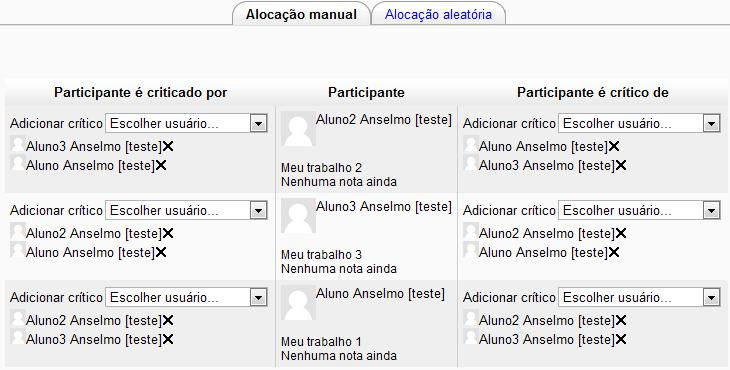
\includegraphics[width=0.5\textwidth]{imagem/cap4_/fig_15.jpg}}
  \caption{Alocação manual}
  \label{fig:aloc_manual}
 \end{center}
\end{figure}

Conforme imagem anterior, que ilustra um exemplo de alocação manual, o usuário “Aluno2” pode ter seu trabalho (Meu trabalho 2) criticado pelos usuários “Aluno” e “Aluno3” e criticar os trabalhos enviados pelos usuários “Aluno” e “Aluno 3”.  Da mesma forma, o usuário “Aluno3” pode ter seu trabalho (Meu trabalho 3) criticado pelos usuários “Aluno2” e “Aluno”, como também criticar os trabalhos enviados pelos usuários “Aluno2” e “Aluno”.

De forma semelhante, o usuário “Aluno” pode ter seu trabalho (Meu trabalho 1) criticado pelos usuários “Aluno2” e “Aluno3”, como também criticar os trabalhos enviados pelos usuários “Aluno2” e “Aluno3”. Para modificar manualmente essa configuração, basta excluir o usuário desejado clicando-se no ícone  correspondente ou no botão seletor escolher usuário.

Para alocar a interação de avaliações entre os alunos de forma aleatória, ou seja, de forma automática, deve-se clicar em
Alocação aleatória, conforme a figura (\ref{fig:aloc_aletoria}). Em seguida devem-se configurar as seguintes opções: modalidade de grupo, número de críticos por envio ou número de críticos por participante, se desejar poderá remover as alocações atuais, os participantes podem avaliar os trabalhos enviados pelos demais alunos sem terem enviado o seu próprio trabalho e se for possível o participante avaliar seu próprio trabalho.

\begin{figure}[htbp]
 \begin{center}
 \fbox{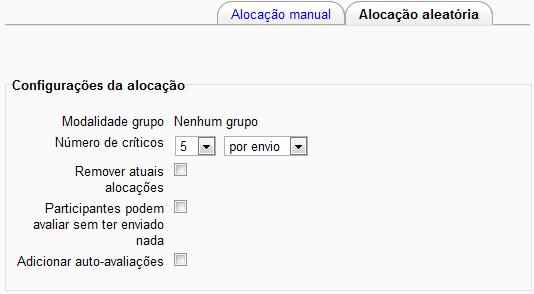
\includegraphics[width=0.5\textwidth]{imagem/cap4_/fig_16.jpg}}
  \caption{Alocação aleatoria}
  \label{fig:aloc_aletoria}
 \end{center}
\end{figure}

\subsection{Fase de avaliação}

Para mudar para a fase de avaliação, o professor deve clicar no ícone fase de avaliação. Nesta fase, os alunos poderão avaliar uns aos outros de acordo com as combinações alocadas na fase anterior (Alocação aleatória), podendo também avaliar o exemplo de arquivo enviado pelo professor.

Em  \textit{grading evaluation} fase o professor irá verificar as avaliações realizadas pelos alunos, bem como as notas atribuídas aos trabalhos enviados e estabelecer a nota final de cada trabalho.

\begin{figure}[htbp]
 \begin{center}
 \fbox{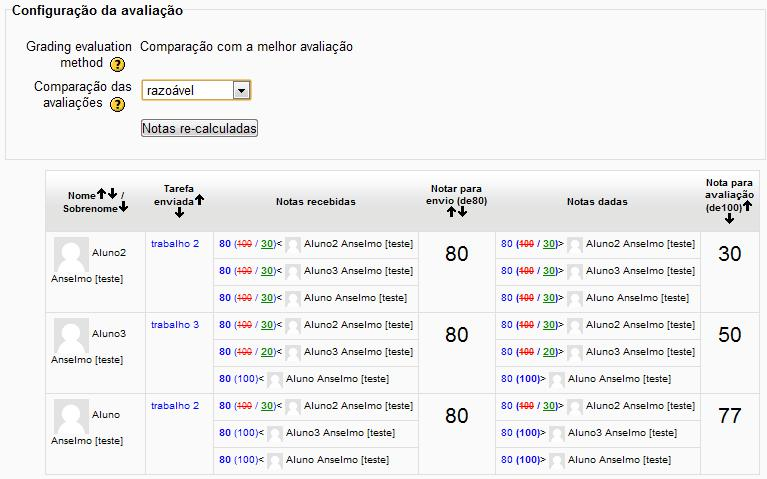
\includegraphics[width=0.5\textwidth]{imagem/cap4_/fig_17.jpg}}
  \caption{Configuração da avaliação}
  \label{fig:config_ava2}
 \end{center}
\end{figure}

A Figura \ref{fig:config_ava2} indica um exemplo de tarefas enviadas por três alunos. Caso seja interesse do professor, existe a possibilidade de alterar manualmente cada nota atribuída ou recebida por cada aluno, para isso, basta clicar no link onde são exibidas as notas nas colunas Notas recebidas e Notas dadas e sobrepor as notas.

A nota final dos alunos é atribuída de forma automática, no entanto, o professor deve estabelecer o grau de rigidez das avaliações. Para isso, deve-se utilizar a opção Comparação das avaliações para selecionar o grau de rigorosidade muito brando, brando, razoável, rigoroso ou muito rigoroso. Quanto mais rigorosa for à comparação, mais similares às avaliações precisam ser para que se possa obter uma nota alta. Após a seleção do grau de rigorosidade, deve-se clicar em Notas re-calculadas, para que o sistema gere as notas automaticamente.

\subsection{Fase errado}

Indica o encerramento da atividade Laboratório de avaliação. Para mudar para esta fase deve-se clicar em encerrado.

\section{Lição}

A lição é uma atividade que busca direcionar o aluno na medida em que ele responda questões. Uma lição baseia-se em uma página contendo texto, imagem ou vídeo e solicita que o aluno, após a leitura, responda uma determinada questão relacionada ao que foi apresentado. As questões apresentadas podem ser de diversos tipos como múltipla escolha, verdadeiro ou falso, de correspondência, dissertativa, etc. Dependendo da resposta do aluno, ele pode ser conduzido a uma nova página contendo outra questão ou ao final da lição, por exemplo.

Para criar a atividade Lição (Figura \ref{fig:add_licao}), temos de ir à disciplina desejada, clicar no botão ativar edição e na semana ou tópico selecionar Lição.

\begin{figure}[htbp]
 \begin{center}
 \fbox{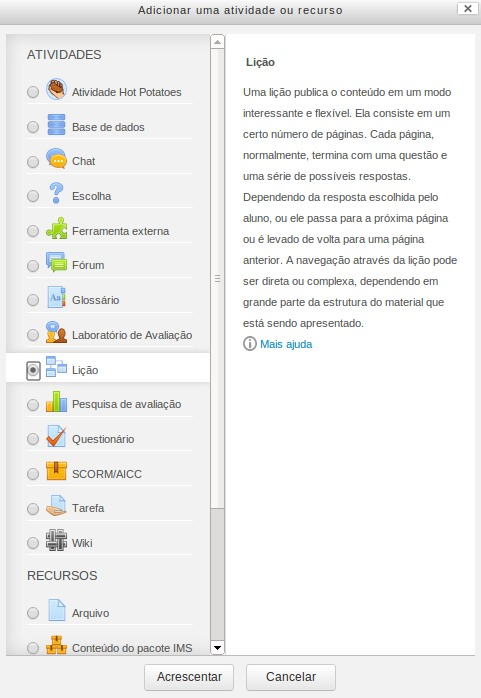
\includegraphics[width=0.3\textwidth]{imagem/cap5/fig75.jpg}}
  \caption{Adicionar lição}
  \label{fig:add_licao}
 \end{center}
\end{figure}

Após esta escolha será apresentado um formulário, conforme a Figura \ref{fig:form_licao}.

\begin{figure}
 \begin{center}
 \fbox{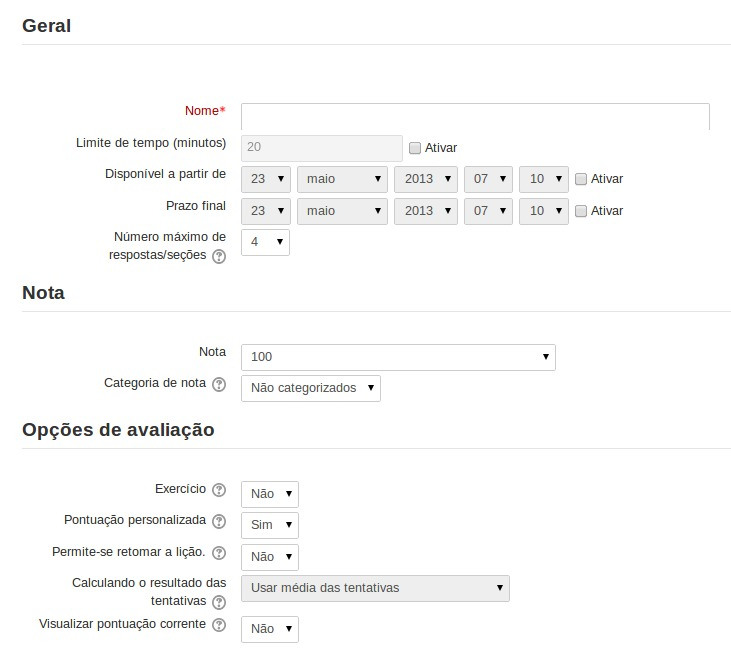
\includegraphics[width=0.5\textwidth]{imagem/cap5/fig76.jpg}}
  \caption{Formulário de lição}
  \label{fig:form_licao}
 \end{center}
\end{figure}

A tabela abaixo descreve os detalhes deste formulário:


\begin{figure}[h]
 \begin{center}
 \fbox{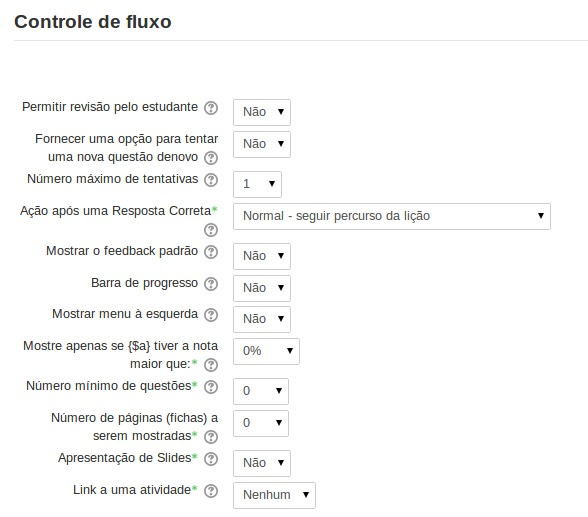
\includegraphics[width=0.5\textwidth]{imagem/cap5/fig77.jpg}}
  \caption{Controle de fluxo}
  \label{fig:cont_fluxo}
 \end{center}
\end{figure}

\begin{longtable}{p{6cm}|p{9cm}}
   \hline
 \rowcolor[rgb]{0.8,0.8,0.8} \textbf{Campos} &  \textbf{Descrição}\\\hline
{Nome} & Nome da atividade que ficará visível na plataforma.\\\hline
{Limite de tempo} & Quantidade de minutos que o aluno terá para responder toda a lição.\\\hline
{Disponível a partir de} & Data de início do período em que a lição ficará disponível.\\\hline
{Prazo final} & Data de fim do período em que a lição ficará disponível.\\\hline
{Número máximo de respostas/sessões} & Número máximo de respostas que o professor pode usar. O valor padrão é 4. Por exemplo, se a lição usar sempre questões VERDADEIRO ou FALSO, é recomendável que este valor seja 2. Esse valor pode ser alterado mesmo após a criação da lição.\\\hline
{Nota} & Valor da nota a ser atribuída para a lição.\\\hline
{Categoria de nota} & Selecionar a categoria de notas do quadro de notas onde a lição será alocada.\\\hline
{Exercício} & Se habilitado, a lição não será avaliada com nota, apenas será criada para fins de estudo.\\\hline
{Pontuação personalizada} & Permite que cada resposta da lição tenha uma pontuação diferenciada. Os valores desta pontuação podem ser negativos ou positivos.\\\hline
{Permite-se retomar a lição} & Determina se os estudantes poderão realizar a lição mais de uma vez ou somente uma vez. O professor pode decidir que a lição contém material que o estudante deve aprender inteiramente.\\\hline
{Calculando o resultado das tentativas} & Caso a opção anterior esteja habilitada, permite escolher se a nota da lição será atribuída como a média das notas das tentativas ou como a nota mais alta.\\\hline
{Visualizar pontuação corrente} & Permite ao aluno visualizar os pontos acumulados até este momento, na medida em que for respondendo as perguntas da lição.\\\hline 
\end{longtable}


A tabela abaixo contém os detalhes referentes a essa tarefa mostrada na Figura \ref{fig:cont_fluxo}.
\begin{longtable}{p{4cm}|p{11cm}}
   \hline
 \rowcolor[rgb]{0.8,0.8,0.8} \textbf{Campos} &  \textbf{Descrição}\\\hline
  {Permitir revisão pelo estudante} & Se habilitada, permite que o estudante volte atrás na lição, caso necessite modificar suas respostas.\\\hline
  {Mostrar botão revisão} & Se habilitada, mostra um botão depois de uma questão respondida incorretamente, permitindo que o estudante tente novamente. Esta opção não é compatível com questões dissertativas.\\\hline
  {Número máximo de tentativas} & Indica o número de tentativas permitidas pelos alunos para realização da lição.\\\hline
  {Ação após uma Resposta Correta} & A ação mais comum é que a lição siga, na medida em que o aluno responda as questões, de acordo com a ordem especificada em sua criação, porém, é possível modificar esta lógica. A lógica mais comum, citada anteriormente, refere-se à opção Normal. A opção Mostrar uma página nunca vista nunca permite que a mesma página seja mostrada duas vezes (mesmo se o estudante não responder a questão associada corretamente). A outra opção não-padrão é Mostrar uma página não respondida, que permite que os estudantes vejam páginas já navegadas, caso não as questões não tenham sido respondidas corretamente.\\\hline
  {Mostrar o feedback padrão} & Se selecionado como \textbf{não}, após a conclusão de uma resposta, o usuário será redirecionado para próxima questão, se selecionado como \textbf{sim}, após a conclusão da questão, será exibido um feedback (“Esta é a resposta correta" ou "Esta é a resposta errada") de acordo com a resposta do aluno.\\\hline
  {Barra de progresso} & Exibe uma barra de progresso na parte inferior da lição.\\\hline
  {Mostrar menu à esquerda} & Mostra uma lista das páginas (Painel de Navegação) na lição. Mostre apenas se $\{\$a\}$ tiver a nota maior que: Esta configuração determina se um estudante deve obter uma certa nota antes de visualizar o menu à esquerda.\\\hline
  {Número mínimo de questões} & Quando uma lição contém um ou mais Painéis de Navegação o professor normalmente deve ativar esse parâmetro. O seu valor determina um limite mínimo do número de questões analisadas quando uma média é calculada, mas sem forçar os estudantes a responderem essa quantidade na lição. Por exemplo, alterando esse parâmetro para, digamos, 20, certificaremos que as notas serão dadas como se os alunos tivessem visto \textbf{no mínimo} esse número de questões. Tomemos o caso de um estudante que só viu uma única ramificação na lição, com 5 páginas, e respondeu corretamente todas as questões associadas a ela. Eles podem preferir terminar a lição. Se esse parâmetro estiver desmarcado, a nota dele poderia ser 5 de 5, que é 100\%. Entretanto, definido para 20, sua nota cairia para 5 de 20, que é 25\%.\\\hline
  {Número de páginas (fichas) a serem mostradas} & O valor padrão é zero, o que significa que todas as Páginas/Fichas são mostradas em uma lição. Fixando o parâmetro com um valor diferente de zero mostra esse número de páginas. Após esse número de Páginas/Fichas terem sido mostradas, o fim da lição é alcançado e a nota é mostrada ao aluno. Se este parâmetro for fixado em um valor maior que o número de páginas na lição, então o final da lição é atingido quando todas as páginas tiverem sido mostradas.\\\hline
  {Apresentação de slides} & permite a exibição das lições como uma apresentação de slide, com largura e altura fixas e cor do plano de fundo alterável.\\\hline
  {Link a uma atividade} & A caixa de seleção contém todas as atividades deste curso. Se uma estiver selecionada, então um link para esta atividade aparecerá no final da Lição.\\\hline
\end{longtable}

\begin{figure}
 \begin{center}
 \fbox{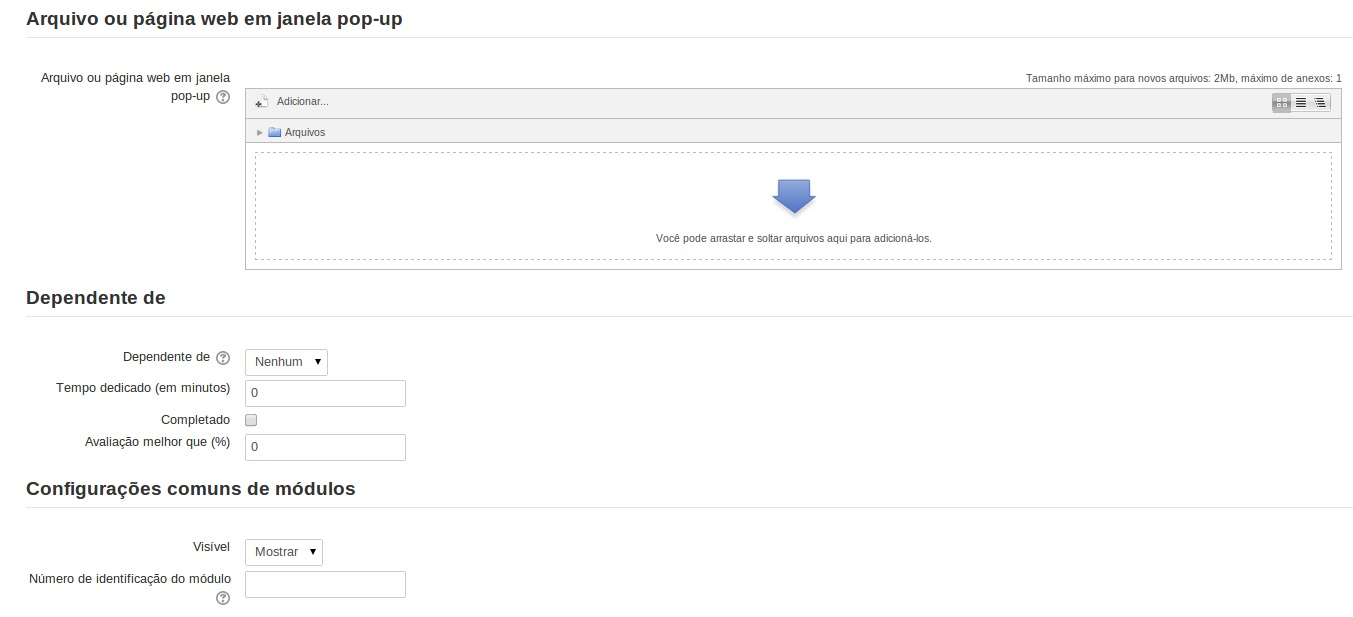
\includegraphics[width=0.5\textwidth]{imagem/cap5/fig78.jpg}}
  \caption{Configurações de arquivo para uma lição}
  \label{fig:conf_arq_licao}
 \end{center}
\end{figure}


A seguinte tabela contém alguns detalhes sobre as configurações de lição (Figura \ref{fig:conf_arq_licao}):

\begin{longtable}{p{4cm}|p{11cm}}
   \hline
 \rowcolor[rgb]{0.8,0.8,0.8} \textbf{Campos} &  \textbf{Descrição}\\\hline
  {Arquivo ou página web em janela pop-up} & No início de uma lição, uma nova janela (pop-up) para uma página web ou um arquivo. Os tipos de arquivo suportados são: mp3, Quicktime, HTML, texto plano, GIF, JPEG e PNG. Outros tipos de formato serão indicados como links para download.\\\hline
  {Depende de} & Este parâmetro possibilita que esta lição dependa do desempenho do aluno em outra lição do mesmo curso. Se as exigências de desempenho não forem atingidas, o aluno não terá acesso a esta lição. As condições para a dependência incluem:\\
  & \textbf{Tempo dedicado:}  O aluno deve gastar esta quantidade de tempo estabelecida na lição requerida;\\
  &\textbf{Completado:}  O aluno deve completar a lição requerida;\\
  &\textbf{Avaliação melhor que:} O aluno deve obter uma nota na lição requerida maior que a especificada aqui;\\
  &\textbf{Visível:}  Se a lição ficará oculta ou não;\\
  &\textbf{Número de identificação do módulo:} Número utilizado para fins de avaliação.\\\hline
\end{longtable}

Após a conclusão e seleção das opções gerais para a criação da atividade Lição, deve-se salvar as configurações realizadas clicando no botão Salvar e voltar para o curso para salvar e retornar para a disciplina ou no botão Salvar e mostrar para salvar e mostrar o recurso criado.

Após a conclusão da etapa anterior, deve-se clicar sobre a lição criada para que as questões possam ser adicionadas. Será exibida a Figura \ref{fig:inserindo_quest}.

\begin{figure}
 \begin{center}
 \fbox{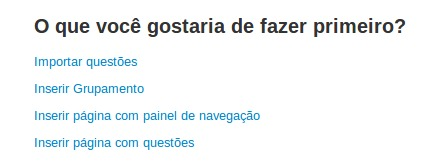
\includegraphics[width=0.4\textwidth]{imagem/cap5/fig79.jpg}}
  \caption{Inserindo questões na lição}
  \label{fig:inserindo_quest}
 \end{center}
\end{figure}

A importação de questões refere-se ao carregamento de questões já criadas previamente. Essas questões devem está presentes no Banco de Questões da disciplina e são as mesmas utilizadas na atividade questionário. Esses tipos de importação não serão abordados nesta sessão, tendo em vista que dependem de etapas anteriores para serem realizadas.

Grupamento refere-se um tipo de divisão entre as questões de uma lição. Em outras palavras, um grupamento pode ser inserido entre as questões de uma lição para dar um novo destino como, por exemplo, o fim da lição. Para inserir um grupamento deve-se clicar em Inserir Grupamento (Figura \ref{fig:inserindo_grup}).

\begin{figure}
 \begin{center}
 \fbox{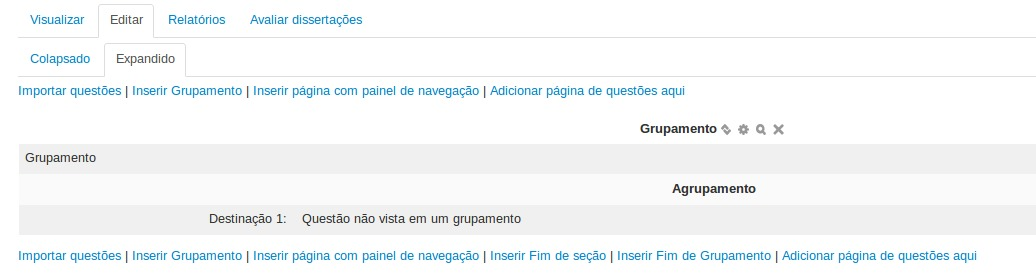
\includegraphics[width=0.5\textwidth]{imagem/cap5/fig80.jpg}}
  \caption{Inserindo grupamento}
  \label{fig:inserindo_grup}
 \end{center}
\end{figure}

A Figura \ref{fig:inserindo_grup} exibe os agrupamentos de questões existentes na lição. Para inserir um novo grupamento deve-se clicar novamente em Inserir Grupamento. Em seguida, um novo grupamento será criado automaticamente. Para editá-lo basta clicar no ícone \includegraphics[width=0.02\textwidth]{imagem/cap5/fig7.jpg} e alterar opções como o título do grupamento e a destinação de cada um deles, como continuar na mesma página (esta página), próxima página, página anterior, fim da lição, questão não vista em um grupamento ou ainda selecionar como destinação um dos agrupamentos já existentes. O formulário de edição do grupamento é exibido na Figura \ref{fig:cap5_53}.

\begin{figure}[htbp]
 \begin{center}
 \fbox{\includegraphics[width=0.5\textwidth]{imagem/cap5/fig53.jpg}}
  \caption{Inserindo páginas com questões}
  \label{fig:cap5_53}
 \end{center}
\end{figure}

Uma página com painel de navegação pode ser comparada a um índice de um livro ou um sumário. Ela pode ser inserida antes ou após a criação de um grupamento. Para inseri-la basta clicar em Inserir página com painel de navegação.  Em seguida, um formulário semelhante à Figura \ref{fig:cap5_54}.
\begin{figure}[htbp]
 \begin{center}
 \fbox{\includegraphics[width=0.5\textwidth]{imagem/cap5/fig54.jpg}}
  \caption{Inserindo páginas com painel de navegação}
  \label{fig:cap5_54}
 \end{center}
\end{figure}
Deve-se preencher o título da página e inserir um conteúdo. Para cada link presente na página, deve-se escrever o texto para o link, escolher um formato de exibição (automática é sempre o mais indicado) e uma destinação. A destinação pode ser selecionada da mesma forma que no grupamento, ou seja, continuar na mesma página (esta página), próxima página, página anterior, fim da lição ou ainda selecionar como destinação um dos agrupamentos já existentes.

Para inserir uma página na lição que contenha alguma questão, basta clicar em inserir página com questões. Uma página semelhante à Figura \ref{fig:cap5_55}.

\begin{figure}[htbp]
 \begin{center}
 \fbox{\includegraphics[width=0.4\textwidth]{imagem/cap5/fig55.jpg}}
  \caption{Inserindo questões}
  \label{fig:cap5_55}
 \end{center}
\end{figure}
Nesta página deve-se selecionar o tipo de questão que se deseja criar. Pode-se escolher entre os tipos Associando, Dissertação, Múltipla Escolha, Numérico, Resposta curta e Verdadeiro/Falso.

A forma de criação de cada tipo de questão não será apresentada nesta sessão, tendo em vista que são muito semelhantes à forma de criação das perguntas da atividade questionário. Desta forma, caso fossem descritas aqui estaria sendo realizada redundância de informação neste documento. Entretanto, em cada tipo de questão deve-se atentar para a opção Destinação, que tem a mesma função apresentada no Grupamento e na página com painel de navegação, ou seja, informar o destino da lição após a escolha da resposta.

Após a criação dos Grupamentos, da página com painel de navegação e das páginas com questões é importante organizá-las. Para isso, deve-se clicar sobre a lição e em seguida na aba Editar. Para uma melhor visualização da disposição das questões da lição aconselha-se clicar sobre a opção Colapsado, conforme Figura \ref{fig:cap5_56}.

\begin{figure}[htbp]
 \begin{center}
 \fbox{\includegraphics[width=0.6\textwidth]{imagem/cap5/fig56.jpg}}
  \caption{Opção colapsada}
  \label{fig:cap5_56}
 \end{center}
\end{figure}
Será apresentado um quadro semelhante à imagem anterior onde é possível identificar a ordem das questões, painéis de navegação e Agrupamentos. É possível ainda verificar as destinações de cada item além de movê-los, editá-los, visualizá-los ou excluí-los de acordo com a necessidade da lição.
Na medida em que os alunos forem respondendo a lição é possível visualizar relatórios da atividade. Para isto, basta clicar sobre a lição e em seguida na aba relatórios. Será exibida uma tela semelhante à Figura \ref{fig:cap5_57}.
\begin{figure}[htbp]
 \begin{center}
 \fbox{\includegraphics[width=0.5\textwidth]{imagem/cap5/fig57.jpg}}
  \caption{Relatórios}
  \label{fig:cap5_57}
 \end{center}
\end{figure}
Como observado na imagem anterior, é possível verificar a porcentagem de acerto de cada aluno que realizou a lição, além da pontuação média, tempo média de resposta, maior e menor percentual de acerto, além do menor e maior tempo de resposta da lição. Estatísticas mais detalhadas, como por exemplo, a resposta individual de cada aluno, pode ser obtida ao clicar em Estatísticas detalhadas.
\subsection{Avaliando questões dissertativas}
Caso alguma questão da lição do tipo Dissertação tenha sido atribuída à lição, é possível avaliá-la clicando-se na aba Avaliar dissertações. É possível verificar a resposta dada por cada aluno e atribuir uma pontuação de acordo com a configuração realizada durante o procedimento de criação da questão.

\section{Pesquisa de avaliação}
Esta atividade é composta por vários questionários específicos para ambientes virtuais de aprendizagem, previamente formatados, cujo objetivo é fazer com que os participantes reflitam sobre sua aprendizagem e participação durante o curso.

\subsection{Acrescentando atividade Pesquisa de Avaliação}

Para acrescentar a atividade Pesquisa de Avaliação, deve-se:

\begin{itemize}
\item Na disciplina desejada, clicar no botão \textbf{Ativar Edição}.

\begin{center}\includegraphics[width=0.3\textwidth]{imagem/cap5/fig58.jpg}\end{center}

\item Será apresentado um formulário, conforme imagem:

\begin{center}\includegraphics[width=0.6\textwidth]{imagem/cap5/fig59.jpg}\end{center}
\end{itemize}

\subsubsection{Geral}
\begin{itemize}
\item \textbf{Nome:} Nome da atividade que ficará visível para os estudantes;
\item \textbf{Tipo de pesquisa de avaliação};
\item \textbf{ATTLS versão de 20 itens:} vinte questionamentos objetivos a respeito das atitudes e pensamentos da aprendizagem, como visto na figura abaixo:

\begin{center}\includegraphics[width=0.8\textwidth]{imagem/cap5/fig60.jpg}\end{center}
\item \textbf{Incidentes críticos:} cinco itens subjetivos a respeito de incidentes acontecidos durante o decorrer da disciplina, como mostra a figura abaixo:

\begin{center} \includegraphics[width=0.6\textwidth]{imagem/cap5/fig61.jpg}\end{center}
\item \textbf{COLLES (experiência efetiva):} 26 itens, em sua maioria objetivos, distribuídos em seis áreas (relevância, reflexão crítica, interatividade, apoio dos tutores, apoio dos colegas e compreensão), como pode ser observado na figura abaixo:

\begin{center}\includegraphics[width=0.6\textwidth]{imagem/cap5/fig62.jpg} \end{center}
\item \textbf{COLLES (expectativa e experiência efetiva):} idêntico ao tipo anterior;
\item\textbf{COLLES (expectativas):} Idêntico aos dois tipos anteriores.
\item\textbf{Introdução padrão:} Instruções para o preenchimento do questionário;

\end{itemize}
\subsubsection{Configurações comuns de módulos}
Definir a modalidade de grupo:
\begin{itemize}
\item \textbf{Nenhum grupo:} - Não há subgrupos, todos fazem parte de uma grande comunidade.
\item \textbf{Grupos separados:} Cada membro de grupo pode visualizar apenas seu próprio grupo.
\item\textbf{Grupos visíveis:} Cada membro do grupo trabalha no seu próprio grupo, mas também pode visualizar outros grupos.
\end{itemize}
Definir se a atividade ficará visível ou oculta para os estudantes através da opção Visível;
Caso necessário, preencher o número de identificação do módulo para fins de avaliação;
Salvar as configurações realizadas clicando no botão \textbf{Salvar e voltar ao curso}  para salvar e retornar para a disciplina ou no botão \textbf{Salvar e mostrar}, para salvar e mostrar a atividade recurso criada
\subsection{Relatórios}
Após o preenchimento da pesquisa de avaliação por parte dos estudantes, é possível verificar alguns gráficos que exemplificam relatórios de desempenho do curso em relação a vários aspectos.
Para ter acesso a esses gráficos, basta clicar sobre a Pesquisa de Avaliação desejada e em seguida em \textbf{Ver X respostas}, no canto superior direito, onde \textbf{X} representa o número de estudantes que responderam a pesquisa.
Um exemplo de gráfico apresentado pela pesquisa de avaliação é exibido na Figura \ref{fig:cap5_63}.

\begin{figure}[htbp]
 \begin{center}
 \fbox{\includegraphics[width=0.5\textwidth]{imagem/cap5/fig63.jpg}}
  \caption{Relatório}
  \label{fig:cap5_63}
 \end{center}
\end{figure}
Clicando-se sobre o gráfico é possível obter novos relatórios relacionados a aspectos distintos.
\section{Questionário}
A atividade questionário auxilia professores e tutores a avaliarem seus alunos por meio de vários tipos de perguntas criadas a partir de um banco de questões. A configuração desta atividade é feita pelo professor, podendo configurá-la com uma ou mais tentativas, além de optar por fornecer feedback e/ou mostrar as respostas corretas aos alunos. A avaliação é feita automaticamente de acordo com o tipo de questão adicionada, permitindo que o professor tenha um trabalho mínimo ao criar e corrigir suas questões. A criação desta atividade é feita a partir do corpo do questionário e o seu banco de questões. Portanto, para se criar um questionário, deve-se:

\begin{enumerate}
 \item \includegraphics[width=0.03\textwidth]{imagem/cap5/fig20.jpg} Criar um banco de questões;
 \item \includegraphics[width=0.03\textwidth]{imagem/cap5/fig21.jpg}  Acrescentar e configurar a atividade questionário. 
\end{enumerate}

\subsection{Criar um banco de questões}

Esta atividade será descrita no Capítulo~\ref{cap6}.

\subsection{Criando um questionário}
Após ativar a edição na disciplina, clicando no botão  \textbf{Ativar Edição}, o professor deverá acrescentar a atividade; No módulo Tarefas, clicar no subgrupo denominado \textbf{Questionário}, conforme a Figura \ref{fig:cap5_22}

\begin{figure}[htbp]
 \begin{center}
 \fbox{\includegraphics[width=0.4\textwidth]{imagem/cap5/fig22.jpg}}
  \caption{Selecionando Questionário}
  \label{fig:cap5_22}
 \end{center}
\end{figure}

\subsection{Configurando um questionário}
Na configuração geral do questionário, o professor preenche os campos do formulário. Além de atribuir um nome e uma descrição, há a possibilidade de ativar um prazo para os alunos enviarem suas respostas, como também um limite de tempo para respondê-lo. Ainda define-se a quantidade de tentativas que o aluno pode responder o questionário. Quando são permitidas diversas tentativas, podem ser configurados quatro modos de cálculo da nota final: Nota mais alta, Nota média, Primeira tentativa e Última tentativa.

Na configuração de layout, o professor define como serão mostradas as questões na página.

\begin{longtable}{p{6cm}|p{9cm}}
     \hline
     \rowcolor[rgb]{0.8,0.8,0.8} \textbf{Campos} &  \textbf{Descrição}\\\hline
    \textbf{Nome}                                                      & Nome do questionário que será visualizado pelos alunos.\\\hline
    \textbf{Introdução}                                                & Uma breve introdução ao questionário\\\hline
    \textbf{Abrir o questionário}                                      &Data e hora a partir da qual o questionário estará disponível para os alunos. Caso essa opção não seja ativada a atividade ficará disponível logo após a criação do questionário.\\\hline
    \textbf{Encerrar o questionário} & Data e hora limite para os alunos responderem o questionário. Caso essa opção não seja ativada o encerramento do questionário fica sem data pré-definida. \\\hline
    \textbf{Limite de tempo}                                           &Se ativado, define o tempo que aluno terá para responder o questionário. As unidades de tempo usadas são: segundos, minutos, horas e dias.\\\hline
    \textbf{Tentativas permitidas}                                     &Define quantas tentativas o aluno poderá utilizar para responder o questionário. O número de tentativas pode ser ilimitado ou um número que varia entre 1 e 10\\\hline
    \textbf{Método de avaliação}                                       &Quando são permitidas diversas tentativas de resposta, podem ser configurados quatro modos de nota final:\\
& \textbf{Nota mais alta} - A nota final é a nota mais alta de todas as tentativas.\\
& \textbf{Nota Média} - Será calculada a média de todas as tentativas.\\
& \textbf{Primeira tentativa} - Apenas os resultados da primeira tentativa, são considerados.\\
& \textbf{Última tentativa} - Apenas o resultado da última tentativa é considerado.\\\hline
\textbf{Ordem das perguntas}                                       &Existem dois modos de ordenação das perguntas:\\
&\begin{itemize}
 \item Como mostrado na tela de exibição - com esta opção, a ordem das perguntas é a mesma definida na configuração das questões.
\item Embaralhar aleatoriamente - com esta opção, a ordem das perguntas é realizada de modo aleatório.
\end{itemize}\\\hline
    \textbf{Nova página}                                               & É a quantidade de questões por páginas. Em questionários muito longos, é preferível que se divida em várias páginas. Podemos exibir todas as questões em uma única página ou dividir um número que varia de 1 a 50 questões por página.\\\hline
    \textbf{Misturar entre as questões}                                &Se esta opção estiver ativa, as partes que compõem as perguntas serão misturadas aleatoriamente toda vez que um estudante iniciar uma tentativa do questionário. Para isso é preciso também que esta opção esteja ativa na configuração das perguntas. Isto dificulta a cópia das respostas entre os alunos.\\\hline
    \textbf{How Questions Behave}                                      &Define o comportamento das questões. Os alunos podem interagir com as perguntas do questionário de várias maneiras diferentes.\\\hline
    \textbf{During the Attempt}                                        &Como as questões se comportam durante a tentativa\\\hline
    \textbf{Após a tentativa}                                          &Como as questões se comportam após a tentativa\\\hline
    \textbf{Mostrar a fotografia do usuário}                           &Se ativado, o nome do aluno e a sua fotografia será exibido na tela durante a tentativa e na revisão, tornando mais fácil a verificação de que o estudante está acessando como ele mesmo em um teste supervisionado.\\\hline
    \textbf{Casas decimais nas avaliações}                             &Este campo permite selecionar o número de algarismos decimais que serão apresentados na classificação de cada tentativa. Por exemplo: o número '0' significa que os números mostrados serão inteiros. o número ‘1’ significa que tem uma casa decimal, e assim sucessivamente. Este modo de exibição não interfere no cálculo da nota.\\\hline
    \textbf{Casas decimais nas avaliações da pergunta}                 & Esta configuração especifica a quantidade de dígitos mostrados após o ponto decimal ao exibir as avaliações para as perguntas individuais.\\\hline
    \textbf{Senha necessária}                                          & É um campo opcional, com ele o professor pode repassar uma senha para alunos que tenham permissão de realizar uma nova tentativa no questionário.\\\hline
    \textbf{Requer endereço de rede}                                   &É um campo opcional de restrição de acesso, nele o professor pode definir o IP da rede na qual os alunos podem acessar o questionário. Os IPs podem ser totais ou parciais. Para definir uma lista de IPs, deve-se separá-los por vírgula.\\\hline
    \textbf{Força demora entre a primeira e a segunda tentativas.}     &Força demora entre a primeira e a segunda tentativas.	Se ativado, o aluno tem que esperar um período de tempo entre a primeira tentativa e a segunda. As unidades de tempo são: segundos, minutos, horas e dias.\\\hline
    \textbf{Força demora entre tentativas posteriores}                 &Se ativado, um aluno tem que esperar este período antes que possa fazer outras tentativas. As unidades de tempo são: segundos, minutos, horas e dias.\\\hline
    \textbf{Feedback geral}                                            &É um texto mostrado para o estudante depois que ele terminou uma tentativa de responder o questionário. O texto que é mostrado pode depender da nota que o estudante obteve.\\\hline
    \textbf{Limite das notas}                                          &\\\hline
    \textbf{Acrescente (Add) outros três campos de feedback}           &Com este botão, acrescentamos mais três campos, cada um com feedback e limite de notas.\\\hline
    \textbf{Modalidade de grupo}                                       &Há três modalidades:
\textbf{Nenhum grupo} – Todos os alunos da disciplina podem trabalhar em conjunto. Todos podem ver e interagir entre si.\\
\textbf{Grupos visíveis} – significa que os alunos participam das atividades apenas com o seu grupo, mas podem ver as atividades dos demais grupos.\\
\textbf{Grupos separados} – O aluno só participa das atividades de seu grupo. Não vê os alunos dos outros grupos. É como se os demais estudantes não existissem para a atividade.\\\hline
    \textbf{Visível}                                                   &Tornar a tarefa visível para os alunos assim que for criada.\\\hline
    \textbf{Número de identificação do módulo}                         &Serve para identificar a atividade para fins de cálculo de avaliação. Se a atividade não estiver inclusa em nenhum cálculo de avaliação, então o campo do número de identificação pode ser deixado em branco.\\\hline
  \label{tab:ConfDisciplina}
  \end{longtable}
  
\subsubsection{Tipos de Perguntas de um questionário}
As questões podem ser criadas no próprio questionário, mas também podem ser inseridas questões que já fazem parte do banco de questões. Iremos explicar como realizar a criação dos diferentes tipos de questões mais adiante, no capítulo que fala sobre o Banco de Questões. Aqui vamos descrever brevemente os diferentes formatos, ou tipos, de questões possíveis de serem construídas.
\subsubsection{Tipo de Questão: Associação}
O tipo Associação é um tipo de questionário, em que estudante que associe itens, a correspondentes alternativas. Estes tipos de questões são úteis na compreensão de vocabulário e fixação de conceitos.

 \textit{\textbf{Adicionando perguntas a um tipo Associação}}

Após configurar o questionário, é preciso adicionar as perguntas: conforme a Figura \ref{fig:cap5_23}.

\begin{figure}[htbp]
 \begin{center}
 \fbox{\includegraphics[width=0.8\textwidth]{imagem/cap5/fig23.jpg}}
  \caption{Adicionando Perguntas}
  \label{fig:cap5_23}
 \end{center}
\end{figure}

\begin{longtable}{p{6cm}|p{9cm}}
     \hline
     \rowcolor[rgb]{0.8,0.8,0.8} \textbf{Campos} &  \textbf{Descrição}\\\hline
	\textbf{Categoria} & A categoria da questão a ser criada  \\\hline
    \textbf{Nome da pergunta} & Nome da pergunta do questionário do tipo associação \\\hline
    \textbf{Texto da questão} & Enunciado da pergunta do tipo associação \\\hline
    \textbf{Marcação padrão} & É o peso de um valor total de uma questão relativo ao questionário \\\hline
    \textbf{Feedback geral} & O professor pode inserir um Feedback (retorno)  geral  ao alunos,  após o encerramento da questão. Este retorno é visualizado por todos os alunos independentemente de sua resposta (correta ou incorreta). \\\hline
    \textbf{Embaralhar} & Se habilitado, a ordem dos pares pergunta-resposta será definida aleatoriamente toda vez que um estudante iniciar uma tentativa no questionário contendo esta pergunta - contanto que "Misturar entre as questões" na configuração do questionário esteja habilitado.\\\hline
    \textbf{Questão} & Nome de cada questão \\\hline
    \textbf{Resposta} & Resposta. \\\hline
    \textbf{Para cada resposta correta} & Feedback” para respostas corretas. \\\hline
    \textbf{For any partially correct response} & ‘Feedback’ para respostas parcialmente corretas \\\hline
    \textbf{Show de number of correct responses} & Mostrar o número de respostas corretas \\\hline
    \textbf{Para qualquer resposta incorreta} & ‘Feedback’ para respostas incorretas \\\hline
    \textbf{Penalty for any from each incorrect try} & Fator de penalidade – Fração da nota que será subtraída para cada resposta errada. Isso somente é relevante se o questionário estiver rodando em modo adaptativo, onde o estudando pode fazer repetidas respostas às perguntas.  \\\hline
    \textbf{Texto da dica} & Texto com dica\\\hline
    \textbf{Adicionar outra dica} & Adicionar outro(s) texto(s) com dica(s) \\\hline
    \textbf{Tags oficiais} & Etiquetas de assuntos (temas) definidas como padrão do MOODLE. \\\hline
    \textbf{Other tags} & Neste campo, é possível definir etiquetas, por assunto, separadas por vírgulas nas quais deseja listar os textos publicados em seu blog, para fins de organização de suas postagens.\\\hline
\end{longtable}%

\subsubsection{Tipo de Questão: Associação aleatória de respostas curtas}
A associação aleatória de respostas curtas é como a pergunta por Associação, porém criada aleatoriamente a partir de perguntas de resposta curta em uma categoria em particular

 \textit{\textbf{Adicionando perguntas a uma associação aleatória de respostas curtas}}
Após configurar o questionário, é preciso adicionar as perguntas: conforme a Figura \ref{fig:cap5_23}.


\begin{longtable}{p{6cm}|p{9cm}}
     \hline
     \rowcolor[rgb]{0.8,0.8,0.8} \textbf{Campos} &  \textbf{Descrição}\\\hline
    \textbf{Categoria} & A categoria da questão a ser criada.  \\\hline
    \textbf{Nome da Pergunta} & Nome da pergunta do questionário do tipo Respostas curtas.  \\\hline
    \textbf{Texto da questão} & Enunciado da questão do questionário do tipo respostas curtas. \\\hline
    \textbf{Feedback geral} & O professor  pode inserir um  Feedback (retorno)  geral  ao alunos,  após o encerramento da questão. Este retorno é visualizado por todos os alunos independentemente de sua resposta (correta ou incorreta). \\\hline
    \textbf{Tags oficiais} &  Etiquetas de assuntos (temas) definidas como padrão do MOODLE. \\\hline
    \textbf{Other tags} &   Neste campo,  você poderá definir  etiquetas,  por assunto, separadas por vírgulas nas quais deseja listar os textos publicados em seu blog, para fins de organização de suas postagens. \\\hline
\end{longtable}%

\subsubsection{Tipo de Questão: Calculado}
As perguntas calculadas são como perguntas numéricas, mas com os números utilizados sorteados a partir de um conjunto quando o questionário é preenchido.

 \textit{\textbf{Adicionando perguntas a um calculado}}

Após configurar o questionário, é preciso adicionar as perguntas: conforme a Figura \ref{fig:cap5_23}.

\begin{longtable}{p{6cm}|p{9cm}}
     \hline
     \rowcolor[rgb]{0.8,0.8,0.8} \textbf{Campos} &  \textbf{Descrição}\\\hline
    \textbf{Categoria} &  A categoria da questão a ser criada \\\hline
    \textbf{Nome da pergunta} & Nome da pergunta do questionário do tipo calculado. \\\hline
    \textbf{Texto da questão} & Enunciado da questão do questionário do tipo calculado. \\\hline
    \textbf{Marcação padrão} & É o peso de um valor total de uma questão relativo ao questionário.\\\hline
    \textbf{Feedback geral} &  O professor  pode inserir um  Feedback (retorno)  geral  ao alunos,  após o encerramento da questão. Este retorno é visualizado por todos os alunos independentemente de sua resposta (correta ou incorreta). \\\hline
    \textbf{Fórmula de resposta correta} &     Informar a fórmula da resposta     \\\hline
    \textbf{Nota} &         \\\hline
    \textbf{Tolerância} & Determinar a tolerância no erro informado pelo aluno. Como nas questões numéricas é possível permitir uma margem dentro da qual todas as questões são aceitas como corretas. O campo tolerância é usado para isto.  \\\hline
    \textbf{Tipo de tolerância} & Existem diferentes tipos de tolerância: Relativa, Nominal e Geométrica.\\
&\textbf{Relativa:} Um intervalo de tolerância é calculado multiplicando-se a resposta correta por 0,5, isto é, neste caso conseguiremos 100 e assim para esta tolerância a resposta correta deve estar entre 100 e 300(200+-100). Isto é útil se a magnitude da resposta correta pode diferenciar largamente entre valores curingas.\\
&\textbf{Nominal:} Este é o tipo de tolerância mais simples, mas não muito poderoso. A resposta correta deve estar entre 199,5 e 200,5(200 +- 0,5). Este tipo de tolerância pode ser útil se as diferenças entre as diferentes respostas corretas forem pequenas. \\
&\textbf{Geométrica:} O limite superior do intervalo de tolerância é calculado com 200 + 0,5*200 e é o mesmo para o caso de tolerância relativa. O limite inferior é calculado como 200/(1+ 0,5). A resposta correta deve estar entre 133,3 e 300. Isto é útil para cálculos complexos que devem ter grandes tolerâncias onde as tolerâncias relativas de 1 ou mais seriam utilizadas para o limite superior mas claramente não aceitáveis para o limite inferior porque o zero seria transformado na resposta correta para todos os casos.\\\hline
    \textbf{Penalty for each incorrect try} &  Conforme o tipo de questão, você define a penalidade que o aluno irá sofrer, caso ele tenha trocado sua alternativa de resposta em uma nova tentativa, sabendo que a escolha anterior estava incorreta.  \\\hline
    \textbf{Texto da dica} & Texto de dica  \\\hline
    \textbf{Tags oficiais} &  Etiquetas de assuntos (temas) definidas como padrão do MOODLE.\\\hline
    \textbf{Other tags} &  Neste campo, você poderá definir  etiquetas,  por assunto, separadas por vírgulas nas quais deseja listar os textos publicados em seu blog, para fins de organização de suas postagens. \\\hline
\end{longtable}%

\subsubsection{Tipo de Questão: Calculado Simples}

O tipo calculado simples é uma versão mais simples das perguntas calculadas que são como perguntas numéricas, mas com os números utilizados sendo sorteados a partir de um conjunto quando o questionário é preenchido.

 \textit{\textbf{Adicionando perguntas a um calculado simples}}

Após configurar o questionário, é preciso adicionar as perguntas: conforme a Figura \ref{fig:cap5_23}.

\begin{longtable}{p{6cm}|p{9cm}}
     \hline
     \rowcolor[rgb]{0.8,0.8,0.8} \textbf{Campos} &  \textbf{Descrição}\\\hline
 \textbf{Categoria} & A categoria da questão a ser criada  \\\hline
    \textbf{Nome da pergunta} & Nome da pergunta do questionário do tipo Calculado simples.\\\hline
    \textbf{Texto da questão} & Enunciado da questão do questionário do tipo calculado simples.  \\\hline
    \textbf{Marcação padrão} & É o peso de um valor total de uma questão relativo ao questionário.  \\\hline
    \textbf{Feedback geral} & O professor pode inserir um Feedback (retorno)  geral  ao alunos,  após o encerramento da questão. Este retorno é visualizado por todos os alunos independentemente de sua resposta (correta ou incorreta).\\\hline
    \textbf{Fórmula de resposta correta} & Informar a fórmula da resposta \\\hline
    \textbf{Nota} &         \\\hline
    \textbf{Tolerância} & Determinar a tolerância no erro informado pelo aluno. Como nas questões numéricas é possível permitir uma margem dentro da qual todas as questões são aceitas como corretas. O campo tolerância é usado para isto. \\\hline
    \textbf{Tipo de tolerância} &         \\\hline
    \textbf{Penalty for each incorrect try} & Conforme o tipo de questão, você define a  penalidade que o aluno irá sofrer, caso ele tenha trocado sua  alternativa de resposta em uma nova tentativa, sabendo que a escolha anterior estava incorreta.   \\\hline
    \textbf{Texto da dica} & Texto de dica \\\hline
    \textbf{Tags oficiais} & Etiquetas de assuntos (temas) definidas como padrão do MOODLE. \\\hline
    \textbf{Other tags} & Neste campo,  você poderá definir  etiquetas,  por assunto, separadas por vírgulas nas quais deseja listar os textos publicados em seu blog, para fins de organização de suas postagens. \\\hline
\end{longtable}%

\subsubsection{Tipo de Questão: Ensaio}
O tipo ensaio permite uma resposta com algumas frases ou parágrafos. Deve, então, ser avaliada manualmente.

 \textit{\textbf{Adicionando perguntas a um ensaio}}

Após configurar o questionário, é preciso adicionar as perguntas: conforme a Figura \ref{fig:cap5_23}.

\begin{longtable}{p{6cm}|p{9cm}}
     \hline
     \rowcolor[rgb]{0.8,0.8,0.8} \textbf{Campos} &  \textbf{Descrição}\\\hline
    \textbf{Categoria} & A categoria da questão a ser criada \\\hline
    \textbf{Nome da Pergunta} & Nome da pergunta do questionário do tipo Ensaio. \\\hline
    \textbf{Texto da questão} & Enunciado da questão do questionário do tipo ensaio. \\\hline
    \textbf{Marcação padrão} &  É o peso de um valor total de uma questão relativo ao questionário. \\\hline
    \textbf{Feedback geral} &  O professor  pode inserir um  Feedback (retorno)  geral  ao alunos,  após o encerramento da questão. Este retorno é visualizado por todos os alunos independentemente de sua resposta (correta ou incorreta). \\\hline
    \textbf{Formato da resposta} & Define como será o formato da resposta: \\\hline
    \textbf{Tamanho da caixa de entrada} &  Tamanho da caixa de texto. Ela pode ser pré-definida com:
5,10,15,20,25,30,35 ou 40 linhas.
 \\\hline
    \textbf{Permitir anexos} & Esta opção permite anexar arquivos. Existem 4 opções de quantidade de anexos: 1, 2, 3 ou ilimitado.\\\hline
    \textbf{Tags oficiais} & Etiquetas de assuntos (temas) definidas como padrão do MOODLE. \\\hline
    \textbf{Other tags} &  Neste campo,  você poderá definir  etiquetas,  por assunto, separadas por vírgulas nas quais deseja listar os textos publicados em seu blog, para fins de organização de suas postagens. \\\hline
\end{longtable}%

\subsection{Tipo de Questão: Múltipla escolha}
Nesse tipo de pergunta de múltipla escolha, o aluno deve escolher uma resposta correta, dentre várias opções apresentadas.

 \textit{\textbf{Adicionando perguntas a um múltipla escolha}}

Após configurar o questionário, é preciso adicionar as perguntas: conforme a Figura \ref{fig:cap5_23}.

\begin{longtable}{p{6cm}|p{9cm}}
     \hline
     \rowcolor[rgb]{0.8,0.8,0.8} \textbf{Campos} &  \textbf{Descrição}\\\hline
    \textbf{Categoria} & A categoria das questões \\\hline
    \textbf{Nome da Pergunta} & Nome da pergunta do questionário do tipo Múltipla escolha. \\\hline
    \textbf{Texto da questão} & Enunciado da questão do questionário do tipo Múltipla escolha.  \\\hline
    \textbf{Marcação padrão} &É o peso de um valor total de uma questão relativo ao questionário.  \\\hline
    \textbf{Feedback geral} & O professor  pode inserir um  Feedback (retorno)  geral  ao alunos,  após o encerramento da questão. Este retorno é visualizado por todos os alunos independentemente de sua resposta (correta ou incorreta).\\\hline
    \textbf{Uma ou múltiplas respostas} & Define se a questão permite apenas uma resposta correta, ou múltiplas respostas corretas.\\\hline
    \textbf{Misturar as opções} & Se habilitado, então a ordem das respostas será misturada aleatoriamente.\\\hline
    \textbf{Numerar as escolhas} & Esta opção permite numerar as escolhas com diversas opções de escolha:\\
&Letras em  minúsculo: a,b,c...\\
&Letras em maiúsculo: A,B,C...\\
&Algarismos romanos em minúsculo: i,ii,iii...\\
&Algarismos romanos em maiúsculo: I,II,III...\\
&Sem numeração.\\
  \\\hline
    \textbf{Resposta} &  É a resposta da questão. Em cada escolha deve-se colocar uma resposta.  \\\hline
    \textbf{Nota} &  É a nota que deve ser atribuído para a nota da resposta.\\\hline
    \textbf{Feedback} & Feedback é retorno de uma mensagem específica para a escolha de determinada alternativa.  \\\hline
    \textbf{Para cada resposta correta} & É um Feedback (retorno) geral para qualquer resposta correta.\\\hline
    \textbf{For any partially correct response} &É um Feedback (retorno) geral para qualquer resposta parcialmente correta. \\\hline
    \textbf{Options} & Exibe o número de respostas corretas. \\\hline
    \textbf{Para qualquer resposta incorreta} & É um Feedback (retorno) geral para qualquer resposta incorreta. \\\hline
    \textbf{Penalty for each incorrect try} & Conforme o tipo de questão, você define a  penalidade que o aluno irá sofrer, caso ele tenha trocado sua  alternativa de resposta em uma nova tentativa, sabendo que a escolha anterior estava incorreta.  \\\hline
    \textbf{Hint text} & Texto de dica \\\hline
    \textbf{Limpar repostas incorretas} &         \\\hline
    \textbf{Show the number of correct responses} & Mostrar o número de respostas corretas \\\hline
    \textbf{Tags Oficiais} & Etiquetas de assuntos (temas) definidas como padrão do MOODLE. \\\hline
    \textbf{Other tags} &  Neste campo,  você poderá definir  etiquetas,  por assunto, separadas por vírgulas nas quais deseja listar os textos publicados em seu blog, para fins de organização de suas postagens. \\\hline
\end{longtable}%

\subsubsection{Tipo de Questão: Múltipla escolha calculada}
As perguntas de múltipla escolha calculada são como questões de múltipla escolha, cujos elementos de escolha podem incluir resultados da fórmula com valores numéricos que são selecionados aleatoriamente a partir de um conjunto quando o questionário é preenchido.

 \textit{\textbf{Adicionando perguntas a uma múltipla escolha calculada}}

Após configurar o questionário, é preciso adicionar as perguntas: conforme a Figura \ref{fig:cap5_23}.

\begin{longtable}{p{6cm}|p{9cm}}
     \hline
     \rowcolor[rgb]{0.8,0.8,0.8} \textbf{Campos} &  \textbf{Descrição}\\\hline
    \textbf{Categoria} & A categoria das questões \\\hline
    \textbf{Nome da pergunta} & Nome da pergunta do questionário do tipo escolha calculada.\\\hline
    \textbf{Texto da questão} & Enunciado da questão do questionário do tipo calculada. \\\hline
    \textbf{Marcação padrão} & É o peso de um valor total de uma questão relativo ao questionário. \\\hline
    \textbf{Feedback geral} & O professor  pode inserir um  Feedback (retorno)  geral  ao alunos,  após o encerramento da questão. Este retorno é visualizado por todos os alunos independentemente de sua resposta (correta ou incorreta). \\\hline
    \textbf{Misturar as opções} & Se ativado, a ordem das respostas será misturada aleatoriamente para cada tentativa, contanto que 'Misturar entre as questões' também esteja habilitado na configuração do questionário. \\\hline
    \textbf{Numerar as escolhas?} & Indicar como as escolhas serão listadas. Ex: A, B, C ou I, II, III  \\\hline
    \textbf{Penalty for each incorrect try} & Conforme o tipo de questão, você define a  penalidade que o aluno irá sofrer, caso ele tenha trocado sua  alternativa de resposta em uma nova tentativa, sabendo que a escolha anterior estava incorreta.  \\\hline
    \textbf{Texto da dica} & Texto de dica  \\\hline
    \textbf{Show the number of correct responses} & Mostrar o número de respostas corretas  \\\hline
    \textbf{Tags oficiais} & Etiquetas de assuntos (temas) definidas como padrão do MOODLE.  \\\hline
    \textbf{Other tags} & Neste campo, você poderá definir  etiquetas,  por assunto, separadas por vírgulas nas quais deseja listar os textos publicados em seu blog, para fins de organização de suas postagens. \\\hline
\end{longtable}%

\subsubsection{Tipo de Questão: Numérico}
Questões do tipo Numérico são muito semelhantes às questões do tipo Resposta breve, mas usadas para resultados numéricos. Pode-se criar questões envolvendo equações, com respostas que devem ser números dentro de uma margem de erro preestabelecida. Caso use números decimais utilize ponto como separador das casas decimais.

 \textit{\textbf{Adicionando perguntas a um numérico}}

Após configurar o questionário, é preciso adicionar as perguntas: conforme a Figura \ref{fig:cap5_23}.

\begin{longtable}{p{6cm}|p{9cm}}
     \hline
     \rowcolor[rgb]{0.8,0.8,0.8} \textbf{Campos} &  \textbf{Descrição}\\\hline
    \textbf{Categoria} & A categoria das questões \\\hline
    \textbf{Nome da pergunta} & Nome da pergunta do questionário do tipo numérico. \\\hline
    \textbf{Texto da questão} & Enunciado da questão do questionário do tipo numérico \\\hline
    \textbf{Marcação padrão} & É o peso de um valor total de uma questão relativo ao questionário. \\\hline
    \textbf{Feedback geral} &  Se ativado, define o tempo que aluno terá para responder o questionário. As unidades de tempo são: segundos, minutos, horas e dias. \\\hline
    \textbf{Feedback} & Feedback é retorno de uma mensagem específica para a escolha de determinada alternativa. \\\hline
    \textbf{Penalty for each incorrect try  } &  Conforme o tipo de questão, você define a  penalidade que o aluno irá sofrer, caso ele tenha trocado sua  alternativa de resposta em uma nova tentativa, sabendo que a escolha anterior estava incorreta \\\hline
    \textbf{Texto da dica} &         \\\hline
    \textbf{Tags oficiais} &  Etiquetas de assuntos (temas) definidas como padrão do MOODLE. \\\hline
    \textbf{Other tags} & Neste campo você poderá definir  etiquetas,  por assunto, separadas por vírgulas nas quais deseja listar os textos publicados em seu blog, para fins de organização de suas postagens. \\\hline
\end{longtable}%

\subsubsection{Tipo de Questão: Resposta curta}
Questões do tipo resposta curta requerem que o aluno digite uma resposta para uma questão. A resposta pode ser uma palavra em uma frase e deve coincidir com a palavra adequada ao contexto, escolhida pelo professor. É uma boa idéia escolher uma resposta curta para evitar erros não intencionais. Além da seção geral configurada, outros ajustes devem ser feitos:

 \textit{\textbf{Adicionando perguntas a resposta curta}}

Após configurar o questionário, é preciso adicionar as perguntas: conforme a Figura \ref{fig:cap5_23}.

\newpage
\begin{longtable}{p{6cm}|p{9cm}}
     \hline
     \rowcolor[rgb]{0.8,0.8,0.8} \textbf{Campos} &  \textbf{Descrição}\\\hline
    \textbf{Categoria} & A categoria das questões \\\hline
    \textbf{Nome da pergunta} & Nome da pergunta do questionário do tipo resposta curta.  \\\hline
    \textbf{Texto da questão} & Enunciado da questão do questionário do tipo resposta curta \\\hline
    \textbf{Marcação padrão} & É o peso de um valor total de uma questão relativo ao questionário.\\\hline
    \textbf{Feedback geral} & O professor pode inserir um Feedback (retorno)  geral  ao alunos,  após o encerramento da questão. Este retorno é visualizado por todos os alunos independentemente de sua resposta (correta ou incorreta). \\\hline
    \textbf{Sensibilidade a caixa} & É a consideração das diferenças entre maiúsculas e minúsculas.
No, case is unimportant. - esta opção não diferencia letras maiúsculas e minúsculas.
Yes, case must match - esta opção diferencia letras maiúsculas e minúsculas.
\\\hline
    \textbf{Resposta} & É a resposta da questão. Em cada escolha deve-se colocar uma resposta. \\\hline
    \textbf{Nota} &  É a nota que deve ser atribuído para a nota da resposta.\\\hline
    \textbf{Feedback} & Feedback é retorno de uma mensagem específica para a escolha de determinada alternativa. \\\hline
    \textbf{Penalty for each incorrect try} & Conforme o tipo de questão, você define a  penalidade que o aluno irá sofrer, caso ele tenha trocado sua  alternativa de resposta em uma nova tentativa, sabendo que a escolha anterior estava incorreta.  \\\hline
    \textbf{Texto da dica} &         \\\hline
    \textbf{Tags oficiais} &  Etiquetas de assuntos (temas) definidas como padrão do MOODLE. \\\hline
    \textbf{Other tags} & Neste campo você poderá definir  etiquetas,  por assunto, separadas por vírgulas nas quais deseja listar os textos publicados em seu blog, para fins de organização de suas postagens.\\\hline
\end{longtable}%
\subsubsection{Tipo de Questão: Resposta embutida (Cloze)}

O que é um tipo de Resposta embutida (Cloze)

 \textit{\textbf{Adicionando perguntas a Resposta embutida (Cloze)}}

Após configurar o questionário, é preciso adicionar as perguntas: conforme a Figura \ref{fig:cap5_23}.

\begin{longtable}{p{6cm}|p{9cm}}
     \hline
     \rowcolor[rgb]{0.8,0.8,0.8} \textbf{Campos} &  \textbf{Descrição}\\\hline
    \textbf{Categoria} & A categoria das questões \\\hline
    \textbf{Nome da pergunta} &Nome da pergunta do questionário do tipo Resposta embutida.\\\hline
    \textbf{Texto da questão} & Enunciado da questão do questionário do tipo Resposta embutida \\\hline
    \textbf{Feedback geral} & O professor pode inserir um Feedback (retorno)  geral  ao
alunos,  após o encerramento da questão. Este retorno é visualizado por todos os alunos independentemente de sua resposta (correta ou incorreta).
 \\\hline
    \textbf{Tags oficiais} & Etiquetas de assuntos (temas) definidas como padrão do MOODLE. \\\hline
    \textbf{Other tags} & Neste campo,  você poderá definir  etiquetas,  por assunto, separadas por vírgulas nas quais deseja listar os textos publicados em seu blog, para fins de organização de suas postagens. \\\hline
\end{longtable}%


\subsubsection{Tipo de Questão: Verdadeiro / Falso}

No tipo de questionário Verdadeiro / Falso o aluno precisa determinar se uma afirmação é verdadeira ou falsa.

 \textit{\textbf{Adicionando perguntas a Verdadeiro / Falso}}

Após configurar o questionário, é preciso adicionar as perguntas: conforme a Figura \ref{fig:cap5_23}.

\begin{longtable}{p{6cm}|p{9cm}}
     \hline
     \rowcolor[rgb]{0.8,0.8,0.8} \textbf{Campos} &  \textbf{Descrição}\\\hline
    \textbf{Categoria} & A categoria das questões. \\\hline
    \textbf{Nome da Pergunta} & Nome da pergunta do questionário do tipo Verdadeiro /Falso.\\\hline
    \textbf{Texto da questão} & Enunciado da questão do questionário do tipo Verdadeiro / Falso. \\\hline
    \textbf{Marcação padrão} & É o peso de um valor total de uma questão relativo ao questionário.   \\\hline
    \textbf{Feedback geral} &O professor  pode inserir um  Feedback (retorno)  geral  ao
alunos,  após o encerramento da questão. Este retorno é visualizado por todos os alunos independentemente de sua resposta (correta ou incorreta).
\\\hline
    \textbf{Resposta certa} &  Define se a resposta certa da questão será o “verdadeiro” ou o “falso”. \\\hline
    \textbf{Feedback para a opção ‘Verdadeiro’} &Nesta opção, o professor pode definir um comentário específico para a opção escolhida “verdadeiro”.\\\hline
    \textbf{Feedback para a opção ‘Falso’} & Nesta opção, o professor pode definir um comentário específico para a opção escolhida “falso”.\\\hline
    \textbf{Penalty for each incorrect try} & Conforme o tipo de questão, você define a  penalidade que o aluno irá sofrer, caso ele tenha trocado sua  alternativa de resposta em uma nova tentativa, sabendo que a escolha anterior estava incorreta. \\\hline
    \textbf{Tags oficiais} & Etiquetas de assuntos (temas) definidas como padrão do MOODLE. \\\hline
    \textbf{Other tags} & Você poderá definir  etiquetas,  por assunto, separadas por vírgulas nas quais deseja listar os textos publicados em seu blog, para fins de organização de suas postagens. \\\hline
\end{longtable}%

\subsubsection{Tipo de Questão: Descrição}

O tipo Descrição é uma forma de adicionar algumas instruções, rubrica ou outros conteúdos para o teste. É semelhante à maneira como os rótulos são utilizados para adicionar conteúdo à página do curso.

 \textit{\textbf{Adicionando perguntas a uma Descrição}}

Após configurar o questionário, é preciso adicionar as perguntas: conforme a Figura \ref{fig:cap5_23}.

\begin{longtable}{p{6cm}|p{9cm}}
     \hline
     \rowcolor[rgb]{0.8,0.8,0.8} \textbf{Campos} &  \textbf{Descrição}\\\hline
    \textbf{Categoria} & A categoria das questões. \\\hline
    \textbf{Nome da pergunta} & Nome da pergunta do questionário do tipo Descrição.\\\hline
    \textbf{Texto da questão} &Enunciado da questão do questionário do tipo descrição.\\\hline
    \textbf{Feedback geral} &O professor  pode inserir um  Feedback (retorno)  geral  ao alunos,  após o encerramento da questão. Este retorno é visualizado por todos os alunos independentemente de sua resposta (correta ou incorreta). \\\hline
    \textbf{Tags oficiais} & Etiquetas de assuntos (temas) definidas como padrão do MOODLE. \\\hline
    \textbf{Other tags} &  Neste campo,  você poderá definir  etiquetas,  por assunto, separadas por vírgulas nas quais deseja listar os textos publicados em seu blog, para fins de organização de suas postagens. \\\hline
\end{longtable}%

\subsubsection{Resultados e avaliação de um questionário}

O questionário do Moodle avalia automaticamente as questões, de acordo com as configurações do professor ao criar as perguntas. Porém existe um tipo de questão que necessita ser avaliada manualmente pelo professor, ou tutor, por exigir uma resposta dissertativa. No Moodle 2.3 essas questões são do tipo \textbf{ENSAIO}.

Para avaliar um ensaio clica-se no questionário. A seguinte tela Figura \ref{fig:cap5_24}.

\begin{figure}[htbp]
 \begin{center}
 \fbox{\includegraphics[width=0.4\textwidth]{imagem/cap5/fig24.jpg}}
  \caption{Avaliando um ensaio}
  \label{fig:cap5_24}
 \end{center}
\end{figure}

Em Tentativas (o número mostra a quantidade de tentativas até o momento) há um link para outra página onde cada uma das tentativas já concluídas é listada. Nas questões do tipo Ensaio não haverá nota e aparece um link onde se lê \textbf{Requer Avaliação} (Figura \ref{fig:cap5_25}).

\begin{figure}[htbp]
 \begin{center}
 \fbox{\includegraphics[width=0.4\textwidth]{imagem/cap5/fig25.jpg}}
  \caption{Requer Avaliação}
  \label{fig:cap5_25}
 \end{center}
\end{figure}

Ao clicar vê-se a pergunta e a resposta do aluno, em uma nova janela. Abaixo destas há um link \textbf{Fazer comentários ou sobrescrever pontuação}. Para avaliar a resposta do aluno é necessário clicar nele, conforme mostra a Figura \ref{fig:cap5_26}.

\begin{figure}[htbp]
 \begin{center}
 \fbox{\includegraphics[width=0.4\textwidth]{imagem/cap5/fig26.jpg}}
  \caption{Fazer comentários ou sobrescrever pontuação}
  \label{fig:cap5_26}
 \end{center}
\end{figure}

Na página seguinte (Figura \ref{fig:cap5_27}).
\begin{figure}[htbp]
 \begin{center}
 \fbox{\includegraphics[width=0.4\textwidth]{imagem/cap5/fig27.jpg}}
  \caption{Observações da correção}
  \label{fig:cap5_27}
 \end{center}
\end{figure}

Após Gravar a nota a lista de tentativas deste aluno, após atualizar a página, mostrará o Resultado (Figura\ref{fig:cap5_28})

\begin{figure}[htbp]
 \begin{center}
 \fbox{\includegraphics[width=0.4\textwidth]{imagem/cap5/fig28.jpg}}
  \caption{Modalidade}
  \label{fig:cap5_28}
 \end{center}
\end{figure}

A avaliação da questão dissertativa foi completada no questionário.

\section{Modalidade avançada de carregamento de arquivos}

\atencao{Atenção: O material a seguir não foi adaptado para a versão do Moodle 2.4. As figuras são do Moodle 2.3.}

\subsubsection{O que é uma modalidade avançada de carregamento de arquivos}

É uma modalidade de tarefa em que o aluno poderá enviar mais de um arquivo (a quantidade de arquivos é definida pelo professor), em diferentes formatos (imagem, texto, zip. etc.).

\subsubsection{Criando uma modalidade avançada de carregamento de arquivos}

Após ativar a edição na disciplina, o professor deverá acrescentar a atividade; No módulo Tarefas, clicar no subgrupo denominado “Modalidade avançada de carregamento de arquivos”.

\subsubsection{Configurando modalidade avançada de carregamento de arquivos}

Para configurar a Modalidade avançada de carregamento de arquivos, existem alguns parâmetros que necessitam ser configurados. Descrevemos abaixo o significado de cada item. Os itens destacados em vermelho são obrigatórios.

\begin{longtable}{p{6cm}|p{9cm}}
     \hline
     \rowcolor[rgb]{0.8,0.8,0.8} \textbf{Campos} &  \textbf{Descrição}\\\hline
	\textbf{Nome da tarefa} & Nome da tarefa que será visualizada pelos alunos. \\\hline
    \textbf{Descrição} &Uma breve descrição da atividade. \\\hline
    \textbf{Disponível a partir de} & Data e hora pela qual a atividade estará disponível para os alunos. Se o campo de seleção “ativar”, estiver desativado, a atividade estará disponível após a criação.\\\hline
    \textbf{Data de Entrega} & Data e hora máxima pela qual os alunos poderão enviar seus arquivos. Se o campo de seleção “ativar”, estiver desativado, a entrega da atividade fica sem data pré-definida. \\\hline
    \textbf{Impedir envio atrasado} & Se habilitado, possibilita ao aluno, o envio de um a tarefa após a data limite para entrega. O sistema registra o atraso em dias e horas.\\\hline
    \textbf{Nota} & Nota máxima atribuída a atividade. \\\hline
    \textbf{Categoria de nota} &  Se houver categoria de nota criada, ela será exibida no menu suspenso.  \\\hline
    \textbf{Tamanho Máximo} & Tamanho máximo dos arquivos que serão postados pelos alunos. \\\hline
    \textbf{Permitir Cancelamento} & Se habilitado, os alunos podem excluir os arquivos enviados a qualquer momento, antes de serem avaliados.\\\hline
    \textbf{Número máximo de arquivos carregados} & Número máximo de arquivos que os alunos podem carregar, Este número não é visualizado pelo aluno. É preferível que a quantidade de arquivos seja informada na descrição da atividade.\\\hline
    \textbf{Permitir Notas} &Se habilitada, os alunos podem fazer anotações na área de texto. Semelhante ao recurso “texto online”.\\\hline
    \textbf{Esconder a descrição antes da data de abertura} & Se habilitado, a descrição da atividade fica oculta até a data de abertura. \\\hline
    \textbf{Aviso por email aos professores} & Se habilitado, os professores serão notificados através de email a cada envio ou atualização de um arquivo enviado. \\\hline
    \textbf{Habilitar envio para a avaliação} & Habilita para o aluno, um botão “Enviar para a avaliação”. Comunica aos professores que eles terminaram uma tarefa. \\\hline
    \textbf{Modalidade de grupo} & Há três modalidades de grupo:\\
&\textbf{Nenhum grupo –} todos os alunos da disciplina podem trabalhar em conjunto. Todos podem ver e interagir com todos os  alunos. \\
&\textbf{Grupos visíveis –} significa que os alunos participam das atividades apenas com o seu grupo, mas podem ver as atividades dos demais grupos.\\
&\textbf{Grupos separados – }O aluno só participa das atividades de seu grupo. Não vê os alunos dos outros grupos. É como se os demais estudantes não existissem para a atividade.
 \\\hline
    \textbf{Visível} & Se visível, a tarefa se torna visível para os alunos assim que criada.\\\hline
    \textbf{Número de identificação do módulo} & O número de identificação é usado para identificar a atividade para fins de cálculo de avaliação. Se a atividade não estiver inclusa em nenhum cálculo de avaliação então o campo do número de identificação pode ser deixado em branco.\\\hline
\end{longtable}%

\subsubsection{Avaliando a modalidade avançada de carregamento de arquivos}

No canto superior direito da tela, há um link \textbf{Ver X tarefas enviadas} .  Onde o \textbf{X}  representa o quantitativo de tarefas nesta modalidade, enviados pelos alunos.

Uma opção de baixar todos os arquivos com um único clique seria clicar no link \textbf{Fazer o download de todas as tarefas com um arquivo ZIP}, que fica localizado no canto superior direito da tela:

Ao exibir a listagem dos alunos pelo qual realizaram a atividade, há uma coluna da tabela chamada “Status”.
Nesta coluna clicando no link: \textbf{Notas} , aparecerão os quadros para a avaliação do aluno.

Na página da avaliação, no item envio de tarefas, conterá uma lista com o nome e a extensão dos arquivos enviados pelo aluno, nesta modalidade de atividade. Conforme a Figura \ref{fig:cap5_29}.

\begin{figure}[htbp]
 \begin{center}
 \fbox{\includegraphics[width=0.4\textwidth]{imagem/cap5/fig29.jpg}}
  \caption{Envio de Tarefa}
  \label{fig:cap5_29}
 \end{center}
\end{figure}

No quadro de envio de tarefas há um botão chamado Reverter a esboço: Este botão permite a um determinado estudante fazer novas atualizações em sua tarefa como: renomear, fazer download, excluir, mover e enviar um novo arquivo.

Para avaliar um aluno com sua nota, o professor deverá escolher entre a escala de nota definida na criação da atividade. Conforme a Figura \ref{fig:cap5_30}.

\begin{figure}[htbp]
 \begin{center}
 \fbox{\includegraphics[width=0.4\textwidth]{imagem/cap5/fig30.jpg}}
  \caption{Notas}
  \label{fig:cap5_30}
 \end{center}
\end{figure}

No quadro de avaliação, como opção, o professor poderá enviar uma resposta para o aluno utilizando o editor de textos padrão do Moodle. Na opção Arquivos de resposta, o professor terá a opção de enviar para o aluno, um arquivo de resposta em anexo.

Enviar notificação via email: ativando esta opção, o aluno será notificado via email, após a conclusão do feedback.

\begin{figure}[htbp]
 \begin{center}
 \fbox{\includegraphics[width=0.4\textwidth]{imagem/cap5/fig31.jpg}}
  \caption{Avaliando (feedback)}
  \label{fig:cap5_31}
 \end{center}
\end{figure}

\section{Texto online}
\atencao{Atenção: O material a seguir não foi adaptado para a versão do Moodle 2.4. As figuras são do Moodle 2.3.}

\subsection{O que é um texto online}
É uma modalidade de tarefa que permite que os usuários editem um texto, utilizando o editor de texto html padrão do Moodle, que é o TinyMCE. O texto online permite ao professor avaliar, modificar e inserir comentários.  Neste tipo de atividade é possível para o aluno anexar imagens, arquivos de audio e vídeo, emotiocons, caracteres especiais e equações matemáticas.
\subsection{Criando um texto online}

Após ativar a edição na disciplina, o professor deverá acrescentar a atividade; No módulo Tarefas, clicar no subgrupo denominado “Texto online”.

\begin{figure}[!htbp]
 \begin{center}
 \fbox{\includegraphics[width=0.4\textwidth]{imagem/cap5/fig32.jpg}}
  \label{fig:cap5_32}
 \end{center}
\end{figure}

\subsection{Configurando um texto online}
\begin{longtable}{p{6cm}|p{9cm}}
     \hline
     \rowcolor[rgb]{0.8,0.8,0.8} \textbf{Campos} &  \textbf{Descrição}\\\hline
    \textbf{Nome da tarefa} & Nome da tarefa que será visualizada pelos alunos. \\\hline
    \textbf{Descrição} &Uma breve descrição da atividade. \\\hline
    \textbf{Disponível a partir de} & Data e hora pela qual a atividade estará disponível para os alunos. Se o campo de seleção “ativar”, estiver desativado, a atividade estará disponível após a criação.\\\hline
    \textbf{Data de Entrega} & Data e hora máxima pela qual os alunos poderão realizar a atividade “texto online”. Se o campo de seleção “ativar”, estiver desativado, a entrega da atividade fica sem data pré-definida.\\\hline
    \textbf{Impedir envio atrasado} & Se habilitado, possibilita ao aluno, o realizar a tarefa após a data limite para entrega. O sistema registra o atraso em dias e horas.\\\hline
    \textbf{Nota} & Nota máxima atribuída a atividade. \\\hline
    \textbf{Categoria de nota} & Se houver categoria de nota criada, ela será exibida no menu suspenso. \\\hline
    \textbf{Permitir novo Envio} &Se habilitado, os alunos poderão enviar novas versões da mesma tarefa mesmo depois que ela for avaliada. Esta modalidade é interessante, quando o professor quer avaliar o aluno de forma contínua, forçando ao aluno, o aprimoramento do conteúdo do texto.\\\hline
    \textbf{Aviso por email aos professores} &Se habilitado, os professores serão avisados através de email, sempre que os alunos enviarem ou atualizarem o “texto online”.\\\hline
    \textbf{Comentário inserido na frase} & Se habilitado, o envio original será copiado no campo de comentário para que seja mais fácil fazer comentários no texto durante a avaliação (talvez usando uma cor diferente) ou para editar o texto original. \\\hline
    \textbf{Modalidade de grupo} & Há três modalidades de grupo:\\
&\textbf{Nenhum grupo –} todos os alunos da disciplina podem trabalhar em conjunto. Todos podem ver e interagir com todos os  alunos.  Grupos visíveis – significa que os alunos participam das atividades apenas com o seu grupo, mas podem ver as atividades dos demais grupos.\\
&\textbf{Grupos separados –} O aluno só participa das atividades de seu
grupo. Não vê os alunos dos outros grupos. É como se os demais estudantes não existissem para a atividade.
 \\\hline
    \textbf{Visível} & Se visível, a tarefa se torna visível para os alunos assim que criada.\\\hline
    \textbf{Número de identificação do módulo} & O número de identificação,  é usado para identificar a atividade para fins de cálculo de avaliação. Se a atividade não estiver inclusa em nenhum cálculo de avaliação então o campo do número de identificação pode ser deixado em branco. \\\hline
\end{longtable}%

\subsection{Avaliando um texto online}
No canto superior direito da tela, há um link  \textbf{Ver x Tarefas enviadas}. Onde o \textbf{X}  representa o quantitativo de textos online enviados pelos alunos.

Ao exibir a listagem dos alunos pelo qual realizaram a atividade, há uma coluna da tabela chamada “Status”. Nesta coluna clicando no link:\textbf{ Nota }, aparecerão os quadros para a avaliação do aluno.

No quadro de envio de tarefas, é listado o texto online que foi criado e enviado pelo aluno.

Para avaliar um aluno com sua nota, o professor deverá escolher entre a escala de nota definida na criação da atividade. Conforme a Figura \ref{fig:cap5_33}

\begin{figure}[!htbp]
 \begin{center}
 \fbox{\includegraphics[width=0.4\textwidth]{imagem/cap5/fig33.jpg}}
\caption{Atribuindo nota}
  \label{fig:cap5_33}
 \end{center}
\end{figure}

O professor, terá a opção de comentar a atividade realizada pelo aluno no campo feedback, conforme a Figura \ref{fig:cap5_34}.

\begin{figure}[!htbp]
 \begin{center}
 \fbox{\includegraphics[width=0.4\textwidth]{imagem/cap5/fig34.jpg}}
\caption{Feedback atividade}
  \label{fig:cap5_34}
 \end{center}
\end{figure}

Enviar notificação via email: ativando esta opção, o aluno será notificado via email, após a conclusão do feedback.

\section{Envio de arquivo único}
\atencao{Atenção: O material a seguir não foi adaptado para a versão do Moodle 2.4. As figuras são do Moodle 2.3.}

É uma modalidade de tarefa que permite que os alunos enviem um único arquivo de qualquer formato (imagem, texto, zip. etc). Após ativar a edição na disciplina, o professor deverá acrescentar a atividade; No módulo Tarefas, clicar no subgrupo denominado “Envio de arquivo único”.

\begin{figure}[!htbp]
 \begin{center}
 \fbox{\includegraphics[width=0.4\textwidth]{imagem/cap5/fig35.jpg}}
  \label{fig:cap5_35}
 \end{center}
\end{figure}

\begin{longtable}{p{6cm}|p{9cm}}
     \hline
     \rowcolor[rgb]{0.8,0.8,0.8} \textbf{Campos} &  \textbf{Descrição}\\\hline
    \textbf{Nome da tarefa} & Nome da tarefa que será visualizada pelos alunos.\\\hline
    \textbf{Descrição} & Uma breve descrição da atividade. \\\hline
    \textbf{Disponível a partir de} & Data e hora pela qual a atividade estará disponível para os alunos. Se o campo de seleção “ativar”, estiver desativada, a atividade estará disponível após a criação. \\\hline
    \textbf{Data de Entrega} & Data e hora máxima pela qual os alunos poderão enviar seu arquivo. Se o campo de seleção “ativar”, estiver desativada, a entrega da atividade fica sem data pré-definida. \\\hline
    \textbf{Impedir envio atrasado} & Se habilitado, possibilita ao aluno, o envio de um a tarefa após a data limite para entrega. O sistema registra o atraso em dias e horas.\\\hline
    \textbf{Nota} &  Nota máxima atribuída à atividade.\\\hline
    \textbf{Categoria de nota} & Se houver categoria de nota criada, ela será exibida no menu suspenso.\\\hline
    \textbf{Permitir novo Envio} & Se habilitado, os alunos poderão enviar novas versões da mesma tarefa mesmo depois que ela for avaliada. Esta modalidade é interessante, quando o professor quer avaliar o aluno de forma contínua, forçando ao aluno, o aprimoramento do conteúdo do texto.\\\hline
    \textbf{Aviso por email aos professores} & Se habilitado, os professores serão avisados através de email sempre que os alunos enviarem ou atualizarem o envio de arquivo único.        \\\hline
    \textbf{Tamanho máximo} & Tamanho máximo do arquivo que será postado pelos alunos.\\\hline
    \textbf{Modalidade grupo} & Há três modalidades de grupo:\\
&\textbf{Nenhum grupo –} todos os alunos da disciplina podem trabalhar em conjunto. Todos podem ver e interagir com todos os  alunos. \\
&\textbf{Grupos visíveis –} significa que os alunos participam das atividades apenas com o seu grupo, mas podem ver as atividades dos demais grupos.\\
&\textbf{Grupos separados –} O aluno só participa das atividades de seu grupo. Não vê os alunos dos outros grupos. É como se os demais estudantes, de outros grupos, não existissem na atividade.
 \\\hline
    \textbf{Visível} &Se visível, a tarefa se torna visível para os alunos assim que criada. \\\hline
    \textbf{Número de identificação do módulo} & O número de identificação, é usado para identificar a atividade para fins de cálculo de avaliação. Se a atividade não estiver inclusa em nenhum cálculo de avaliação então o campo do número de identificação pode ser deixado em branco.\\\hline
\caption{Preenchimento de envio de arquivo único}
\end{longtable}%

\subsection{Avaliando um envio de arquivo único}
No canto superior direito da tela, há um link ver tarefas enviadas, onde o   representa o quantitativo de tarefas nesta modalidade, enviado pelos alunos. Uma opção de baixar todos os arquivos com um único clique seria clicar no link Fazer download de todas as tarefas como um arquivo ZIP, localizado no canto superior direito da tela.

Ao exibir a listagem dos alunos pelo qual realizaram a atividade, há uma coluna da tabela chamada “Status”. Nesta coluna clicando no link: Nota aparecerão os quadros para a avaliação do aluno.

Na página da avaliação, no item envio de tarefas, conterá uma lista com o nome e a extensão do arquivo enviado pelo aluno, nesta modalidade de atividade. Conforme a Figura \ref{fig:cap5_36}

\begin{figure}[!htbp]
 \begin{center}
 \fbox{\includegraphics[width=0.4\textwidth]{imagem/cap5/fig36.jpg}}
\caption{Envio de tarefas}
  \label{fig:cap5_36}
 \end{center}
\end{figure}

Para avaliar um aluno com sua nota, o professor deverá escolher entre a escala de nota definida na criação da atividade. Conforme a Figura \ref{fig:cap5_37}.

\begin{figure}[!htbp]
 \begin{center}
 \fbox{\includegraphics[width=0.4\textwidth]{imagem/cap5/fig37.jpg}}
\caption{Envio de notas}
  \label{fig:cap5_37}
 \end{center}
\end{figure}

O professor, terá a opção de comentar a atividade realizada pelo aluno no campo feedback, conforme a Figura \ref{fig:cap5_38}.
\begin{figure}[!htbp]
 \begin{center}
 \fbox{\includegraphics[width=0.4\textwidth]{imagem/cap5/fig38.jpg}}
\caption{Avaliação}
  \label{fig:cap5_38}
 \end{center}
\end{figure}
Na opção “Arquivos de resposta”, o professor terá a opção de enviar para o aluno, um arquivo de resposta em anexo. No campo de seleção “Enviar notificação via email”, quando ativando esta opção, o aluno será notificado via email, após a conclusão do feedback.

\section{Atividade offline}
\atencao{Atenção: O material a seguir não foi adaptado para a versão do Moodle 2.4. As figuras são do Moodle 2.3.}

\subsection{O que é uma atividade offline}
É uma modalidade de tarefa que não será realizada online, nem enviada como envio de arquivo. Os alunos podem consultar o enunciado da tarefa, porém não poderá enviá-la pela plataforma, normalmente utilizada para colocar no Moodle resultados de avaliações presenciais, realizadas e entregues nos polos.
\subsection{Criando uma atividade offline}
Após ativar a edição na disciplina, o professor deverá acrescentar a atividade; No módulo Tarefas, clicar no subgrupo denominado “Atividade offline”, conforme a Figura \ref{fig:cap5_39}.

\begin{figure}[!htbp]
 \begin{center}
 \fbox{\includegraphics[width=0.4\textwidth]{imagem/cap5/fig39.jpg}}
\caption{Atividade Offiline}
  \label{fig:cap5_39}
 \end{center}
\end{figure}
\subsection{Configurando uma atividade offline}

Para configurar a atividade offline, existem alguns parâmetros que necessitam ser configurados. Descrevemos abaixo o significado de cada item. Os itens destacados em vermelho são obrigatórios.

\begin{longtable}{p{6cm}|p{9cm}}
     \hline
     \rowcolor[rgb]{0.8,0.8,0.8} \textbf{Campos} &  \textbf{Descrição}\\\hline
    \textbf{Nome da tarefa} & Nome da tarefa que será visualizada pelos alunos. \\\hline
    \textbf{Descrição} &Uma breve descrição da atividade. \\\hline
    \textbf{Disponível a partir de} &Não considerar este item, visto que a atividade será realizada extraclasse.\\\hline
    \textbf{Data de Entrega} &Não considerar este item, visto que a atividade será realizada extraclasse. \\\hline
    \textbf{Impedir envio atrasado} & Não considerar este item, visto que a atividade será realizada extraclasse. \\\hline
    \textbf{Nota} & Nota máxima atribuída a atividade.\\\hline
    \textbf{Categoria de nota} & Se houver categoria de nota criada, ela será exibida no menu suspenso.\\\hline
    \textbf{Modalidade grupo} & Há três modalidades de grupo:\\
& \textbf{Nenhum grupo} – todos os alunos da disciplina podem trabalhar em conjunto. Todos podem ver e interagir com todos os  alunos. \\
& \textbf{Grupos visíveis} – significa que os alunos participam das atividades apenas com o seu grupo, mas podem ver as atividades dos demais grupos.\\
& \textbf{Grupos separados} – O aluno só participa das atividades de seu grupo. Não vê os alunos dos outros grupos. É como se os demais estudantes, de outros grupos, não existissem na atividade.\\
\\\hline
    \textbf{Visível} &Se visível, a tarefa se torna visível para os alunos assim que criada.\\\hline
    \textbf{Número de identificação do módulo} & O número de identificação,  é usado para identificar a atividade para fins de cálculo de avaliação. Se a atividade não estiver inclusa em nenhum cálculo de avaliação então o campo do número de identificação pode ser deixado em branco. \\\hline
\caption{Preenchimento da cofiguração da atividade offline}
\end{longtable}%

\section{Avaliando uma atividade offline}
\atencao{Atenção: O material a seguir não foi adaptado para a versão do Moodle 2.4. As figuras são do Moodle 2.3.}


No canto superior direito da tela, há um link  \textbf{Ver avaliação e Feedback}. Onde o professor poderá avaliar o desempenho do aluno nesta atividade offline.

Logo após clicar no link   \textbf{Ver avaliação e Feedback}, o professor poderá avaliar o desempenho do aluno clicando no link “Nota”, que fica localizado na coluna “Status”.
Na página da avaliação, o envio de tarefas, sempre estará em branco, visto que uma atividade offline, o aluno não envia a atividade pela plataforma. Conforme a Figura \ref{fig:cap5_40}.

\begin{figure}[!htbp]
 \begin{center}
 \fbox{\includegraphics[width=0.4\textwidth]{imagem/cap5/fig40.jpg}}
\caption{Envio de tarefas}
  \label{fig:cap5_40}
 \end{center}
\end{figure}
Para avaliar um aluno com sua nota, o professor deverá escolher entre a escala de nota definida na criação da atividade. Conforme a figura  \ref{fig:cap5_41}.

\begin{figure}[!htbp]
 \begin{center}
 \fbox{\includegraphics[width=0.4\textwidth]{imagem/cap5/fig41.jpg}}
\caption{Notas}
  \label{fig:cap5_41}
 \end{center}
\end{figure}
O professor, terá a opção de comentar a atividade realizada pelo aluno no campo feedback, conforme a Figura \ref{fig:cap5_42}.

\begin{figure}[!htbp]
 \begin{center}
 \fbox{\includegraphics[width=0.4\textwidth]{imagem/cap5/fig42.jpg}}
\caption{Avaliação}
  \label{fig:cap5_42}
 \end{center}
\end{figure}

No campo de seleção “Enviar notificação via email”, quando ativando esta opção, o aluno será notificado via email, após a conclusão do feedback.

\section{Wiki}
\subsection{O que é o Wiki}
O Wiki disponibiza documentos produzidos colaborativamente, utilizando  o navegador web.

No Moodle, a atividade Wiki  permite que  os participantes  trabalhem em conjunto, de forma assíncrona, numa mesma página para adicionar, expandir e alterar conteúdos, guardando o histórico dos registros de inserção ou alteração de conteúdo.

Trata-se de uma ferramenta de criação de conteúdos de colaboração com foco no trabalho em grupo, uma vez que permite trabalho web utilizando um simples  editor Html, Creole ou Nwiki  do Moodle.

\subsection{Criando Wikis}
Após ativar a edição na disciplina, o professor deverá acrescentar a atividade; A última opção é a atividade Wiki. Conforme a Figura \ref{fig:cap5_43}.
\begin{figure}[!htbp]
 \begin{center}
 \fbox{\includegraphics[width=0.4\textwidth]{imagem/cap5/fig43.jpg}}
\caption{Wiki}
  \label{fig:cap5_43}
 \end{center}
\end{figure}
\subsection{Configurando uma página Wiki}
Para configurar a página wiki, existem alguns parâmetros que necessitam ser configurados. Descrevemos abaixo o significado de cada item. Os itens destacados em vermelho são obrigatórios.

\begin{longtable}{p{6cm}|p{9cm}}
     \hline
     \rowcolor[rgb]{0.8,0.8,0.8} \textbf{Campos} &  \textbf{Descrição}\\\hline
    \textbf{Nome da wiki} & Nome da wiki que será visualizada pelos alunos. \\\hline
    \textbf{Descrição da wiki} &  Uma breve descrição da wiki. \\\hline
    \textbf{Nome da primeira página} &É o título da primeira página Wiki. \\\hline
    \textbf{Modo wiki} & Determina o poder de edição de uma wiki. Há dois tipos de Wiki:\\
&\textbf{ Wiki colaborativa} - Uma única wiki, em que todos podem editar. \\
& \textbf{Wiki individual} - Cada aluno tem sua wiki, podendo apenas editar em seu espaço Wiki. \\
\\\hline
    \textbf{Formato padrão} &  Existem três formatos de edição de textos wiki:\\
&HTML - Editor de textos padrão do Moodle (TyniMCE).\\
&Creole - Editor com linguagem de marcação Wiki.\\
&Nwiki - Editor similar ao tipo usado no Wikipedia.\\
&Os formatos Creole e Nwiki são similares.\\
  \\\hline
    \textbf{Forçar formato} & Se o habilitado, o formato é forçado . Sendo assim, o usuário fica impossibilitado de escolher outro formato, com o objetivo de editar uma página wiki. \\\hline
    \textbf{Modalidade grupo} & Há três modalidades de grupo:\\
&\textbf{Nenhum grupo }– todos os alunos da disciplina podem trabalhar em conjunto. Todos podem ver e interagir com todos os  alunos. \\
&\textbf{Grupos visíveis} – significa que os alunos participam das atividades apenas com o seu grupo, mas podem ver as atividades dos demais grupos.\\
&\textbf{Grupos separados} – O aluno só participa das atividades de seu grupo. Não vê os alunos dos outros grupos. É como se os demais estudantes, de outros grupos, não existissem na atividade.
\\\hline
    \textbf{Visível} & Se visível, a tarefa se torna visível para os alunos assim que criada. \\\hline
    \textbf{Número de identificação do módulo} & O número de identificação,  é usado para identificar a atividade para fins de cálculo de avaliação. Se a atividade não estiver inclusa em nenhum cálculo de avaliação então o campo do número de identificação pode ser deixado em branco.  \\\hline
\caption{Preenchimento da cofiguração da Wiki}
\end{longtable}%

\subsection{Administrando uma Wiki}
\begin{figure}[!htbp]
 \begin{center}
 \fbox{\includegraphics[width=0.4\textwidth]{imagem/cap5/fig44.jpg}}
\caption{Menu Wiki}
  \label{fig:cap5_44}
 \end{center}
\end{figure}

O objetivo da Wiki, não é avaliar o aluno, e sim a distribuir conhecimentos, sendo assim, a wiki não poderá ser avaliada com uma nota, nem mesmo aparecerá como uma atividade no quadro de notas.

Caso o modo da Wiki escolhido, for o Modo Individual, haverá um menu suspenso no canto superior direito da tela, \textbf{Escolher...} , no qual poderá filtrar o conteúdo da wiki, pelos participantes da disciplina. No caso de uma Wiki

Colaborativa, este menu suspenso é inexistente, visto que todos têm o poder de edição de um único texto.
Para administrar a wiki, o Moodle oferece um menu com abas, para que facilite as operações de manipulação da Wiki, conforme a Figura \ref{fig:cap5_44}.


Descrevemos na Tabela \ref{tab:wiki} o significado de cada item.
\begin{longtable}{p{6cm}|p{9cm}}
     \hline
     \rowcolor[rgb]{0.8,0.8,0.8} \textbf{Campos} &  \textbf{Descrição}\\\hline
    \textbf{Visualizar} &O professor tem o privilégio de visualizam o conteúdo da Wiki. \\\hline
    \textbf{Editar} & O professor tem o privilégio de editar o conteúdo da Wiki.\\\hline
    \textbf{Comentários } & O professor pode tecer comentários na wiki. \\\hline
    \textbf{Histórico} & O histórico, guarda os registros de inserções e alterações de conteúdo, guardando a data e hora, nome do usuário e versão.
Com o histórico, podemos fazer comparações entre conteúdos.
 \\\hline
    \textbf{Mapa} & É no mapa localizamos separadamente itens criados na wiki. Os itens do menu são: Contribuições, Links, Páginas órfãs, Índice das páginas, Lista das páginas, Páginas atualizadas. \\\hline
    \textbf{Files} & Lista os arquivos anexados na wiki.\\\hline
    \textbf{Administration} &Na aba administração, podemos remover páginas e excluir versões de páginas. \\\hline
\caption{Administrando Wiki}
\label{tab:wiki}
\end{longtable}%
